\section{Results and Discussion}
In this section, the results of SDCP performance will be presented along with test scenarios introduced in section III and provide more details in this section. The discussion highlights the advantages and limitations of the proposed platoon system.

The training model for this multi-agent system (SDCP) took 25 million training steps for approximately 11.25 hours with a timescale x10, which is 112.5 hours of training on the real-time scale. Figure 10 shows the mean cumulative reward of the training model for each 20000 training step and the curve is smoothed to make a better visualization of learning mean rewards between exploration and exploitation.


\begin{figure}
    \centering
    %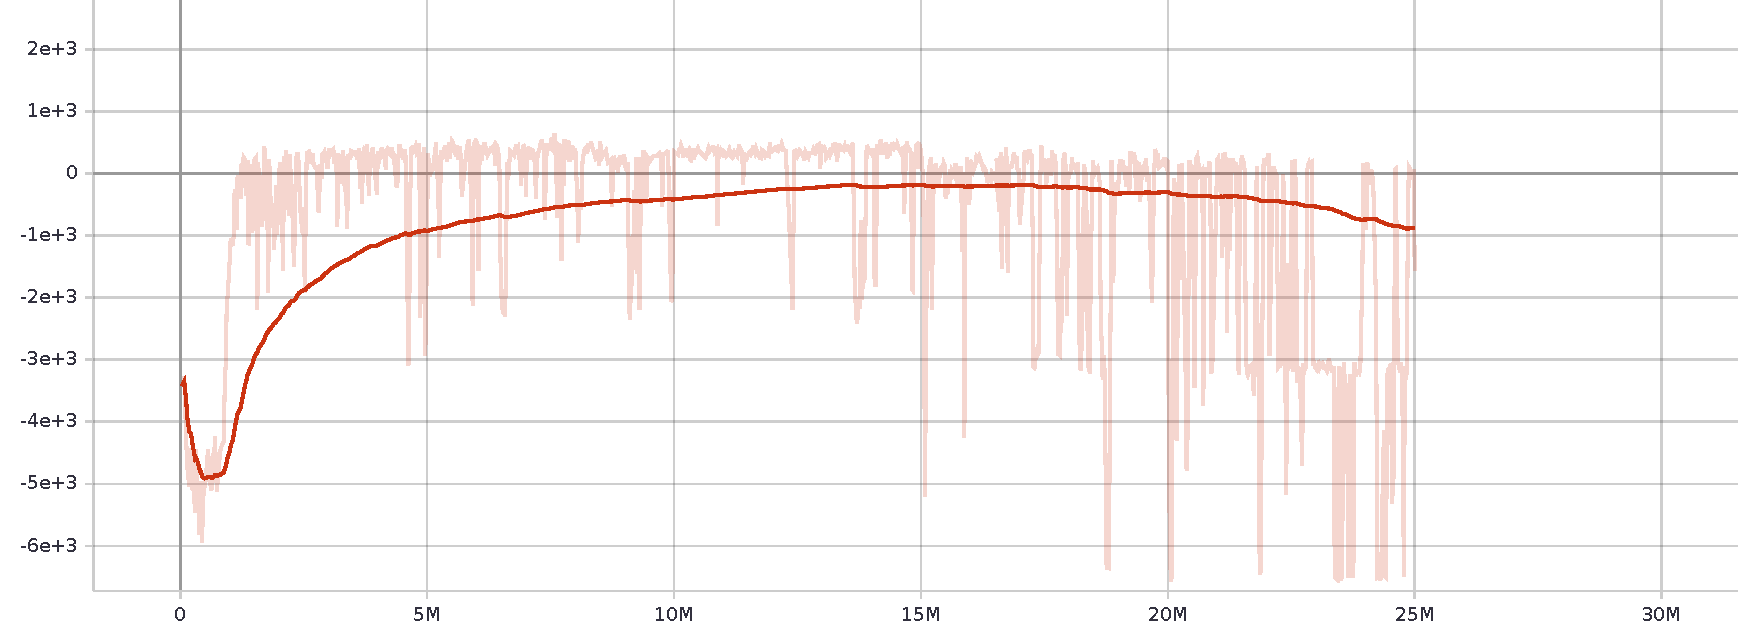
\includegraphics[width=8cm,height=5cm,keepaspectratio]{Figures/CumR.pdf}
    %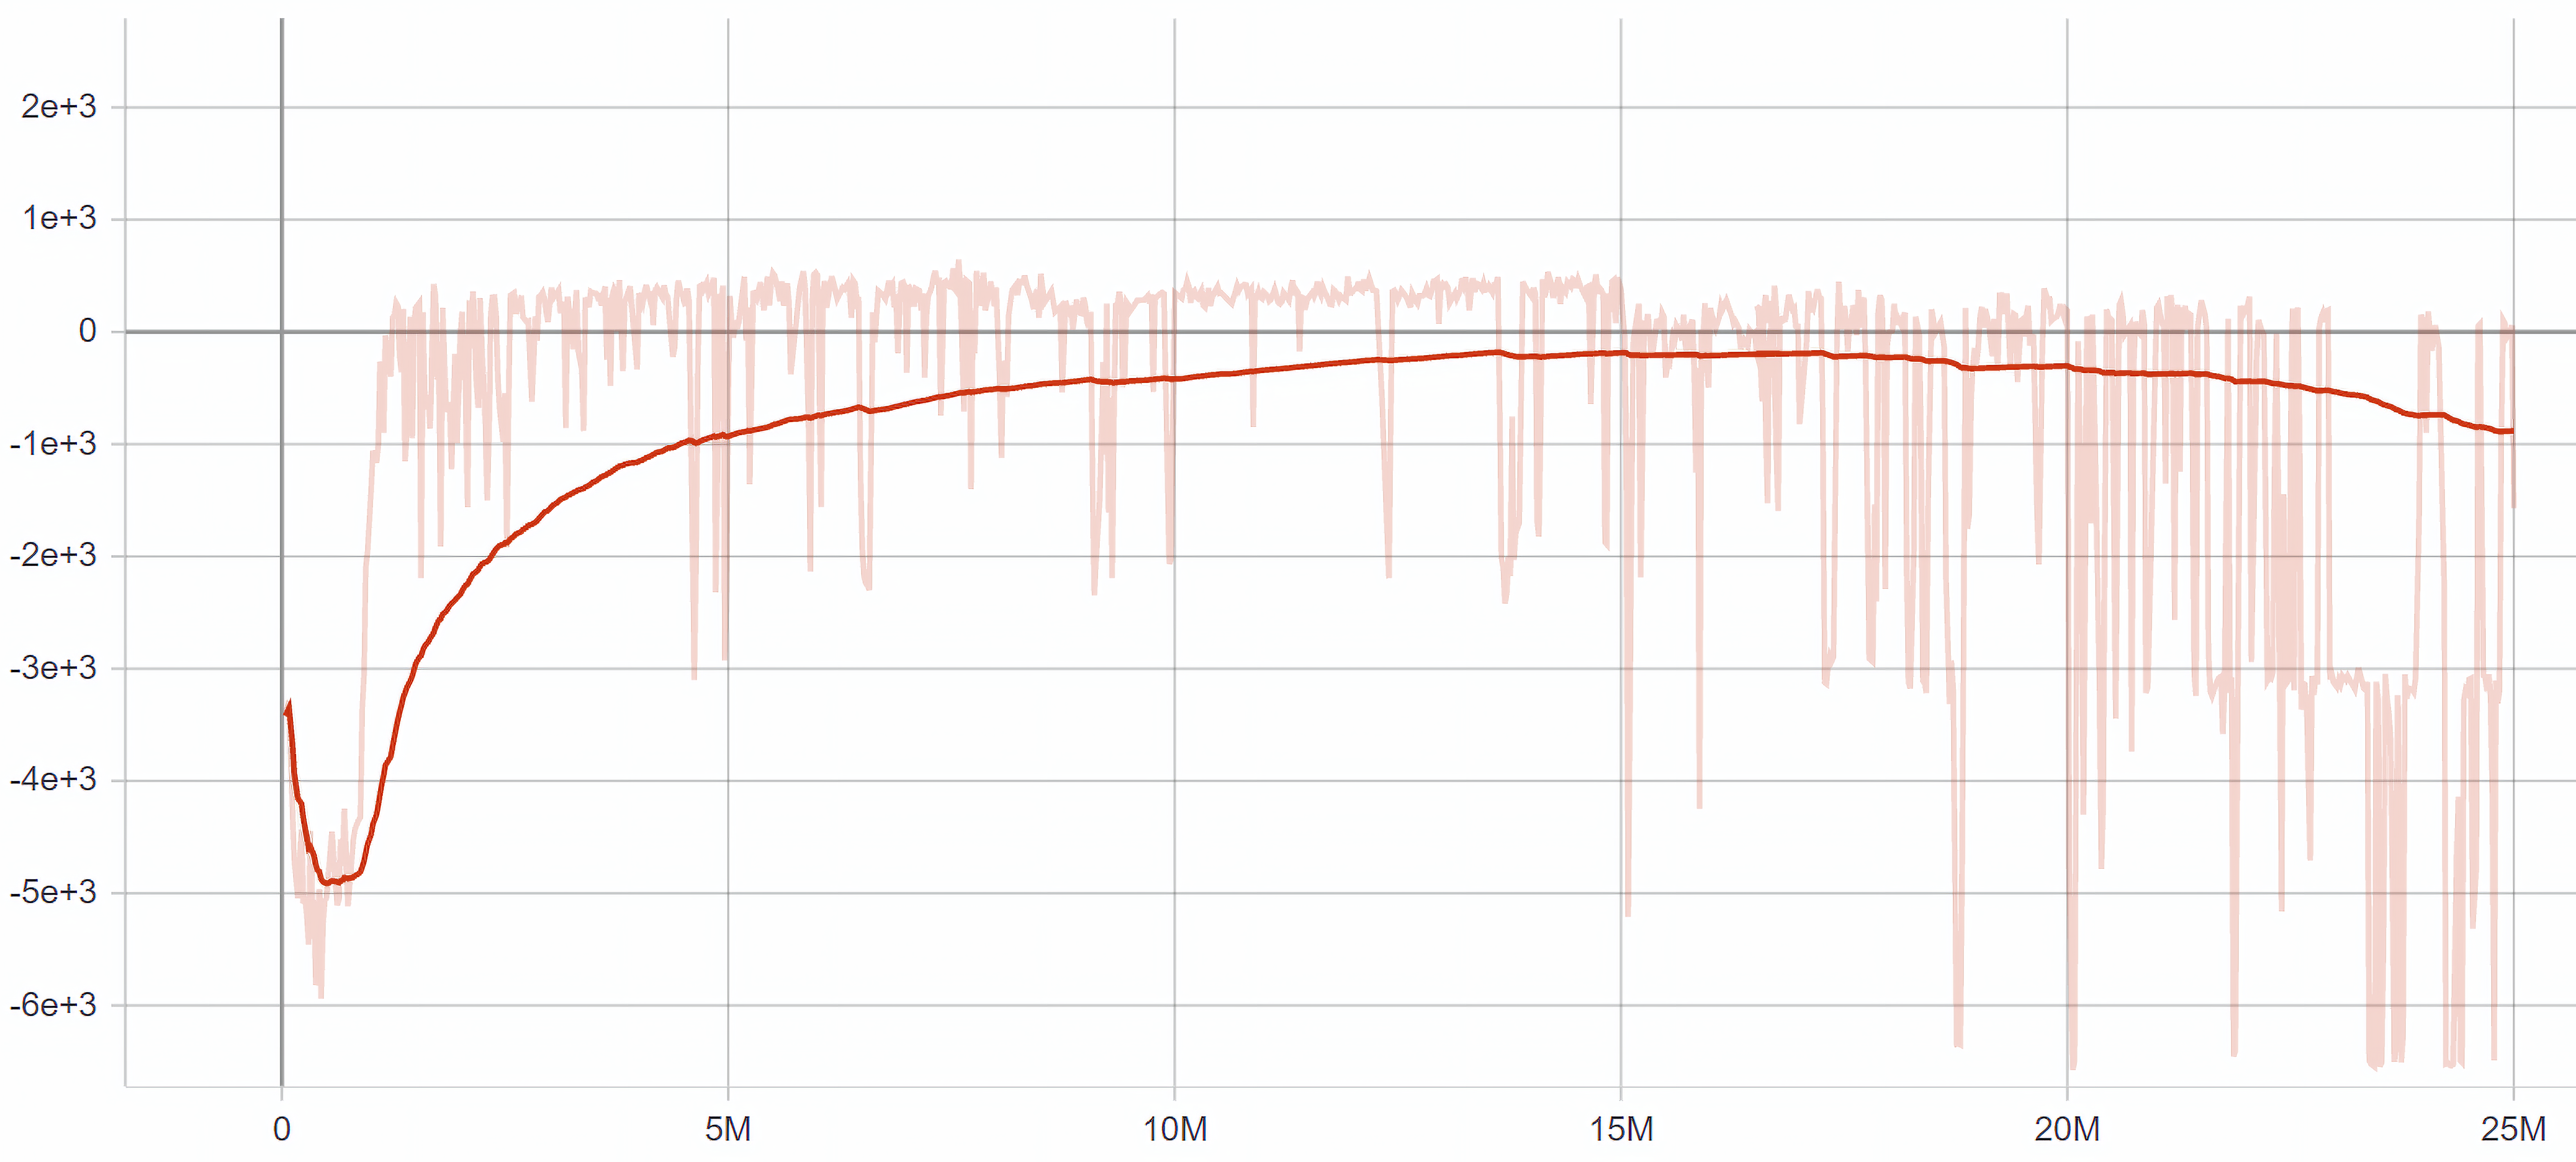
\includegraphics[scale=0.4]{Figures/Tensorboard4.PNG}
    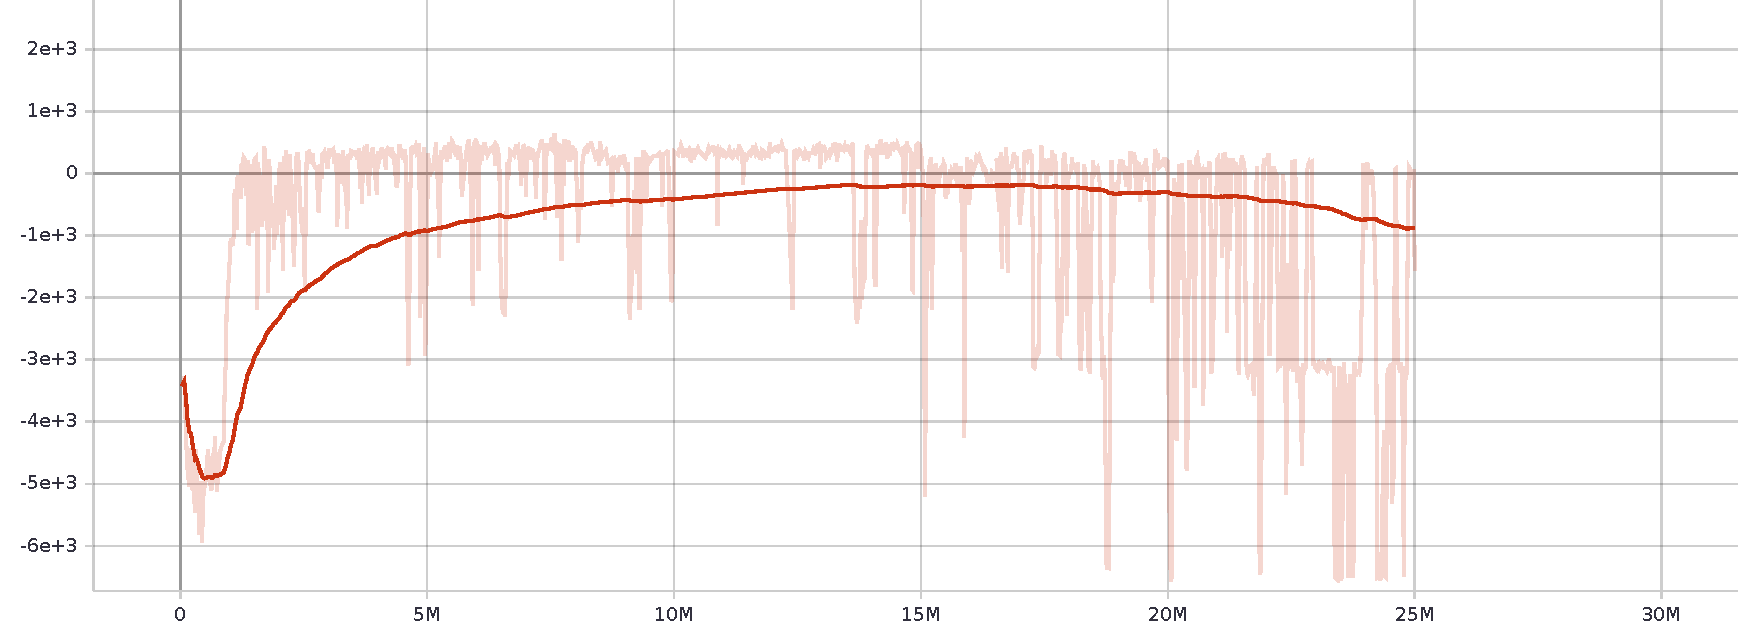
\includegraphics[height=4cm, width=9cm]{Figures/ECumR_compressed.pdf}
    \caption{Mean Cumulative Reward vs Training Steps for the Multi-Agent System}
\end{figure}

\begin{comment}
\begin{figure}
    \centering
    %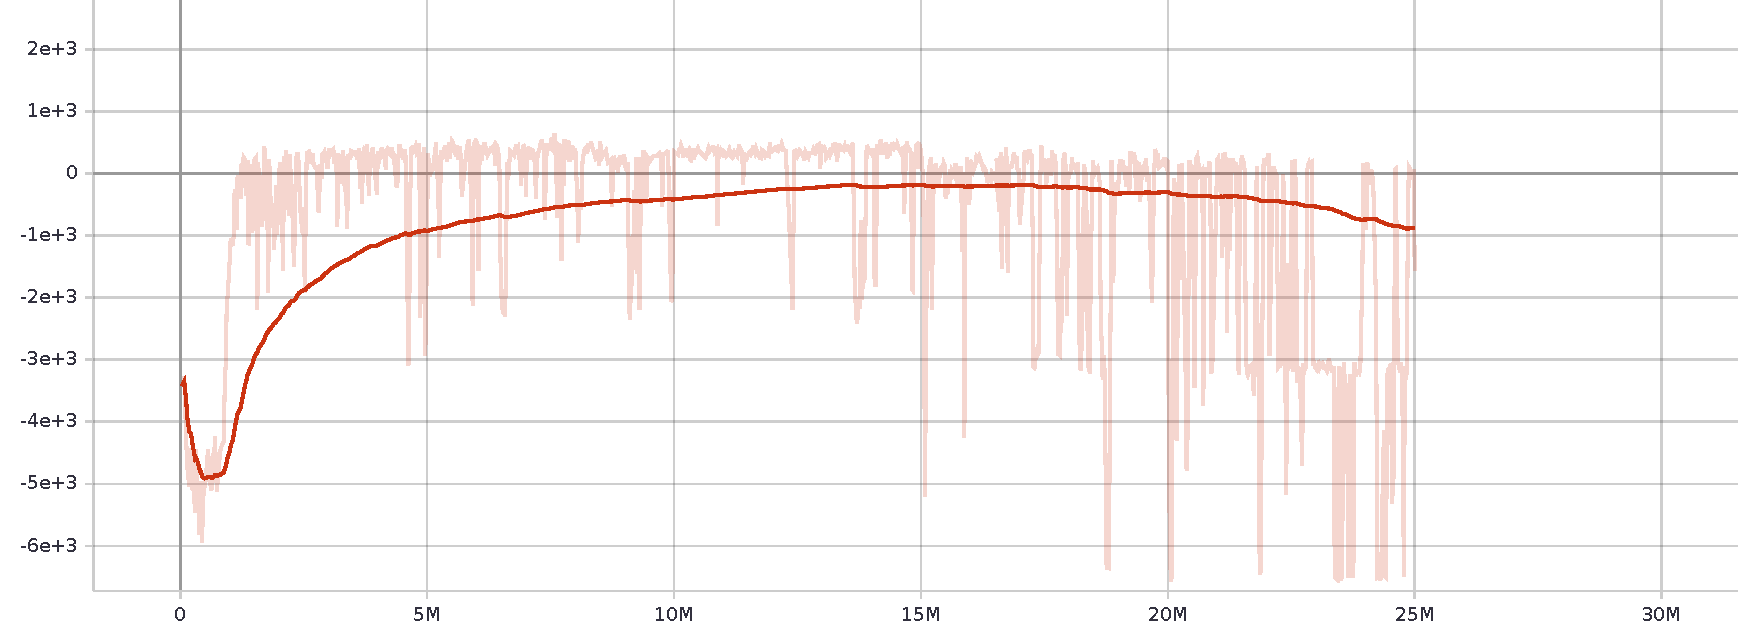
\includegraphics[width=8cm,height=5cm,keepaspectratio]{Figures/CumR.pdf}
    %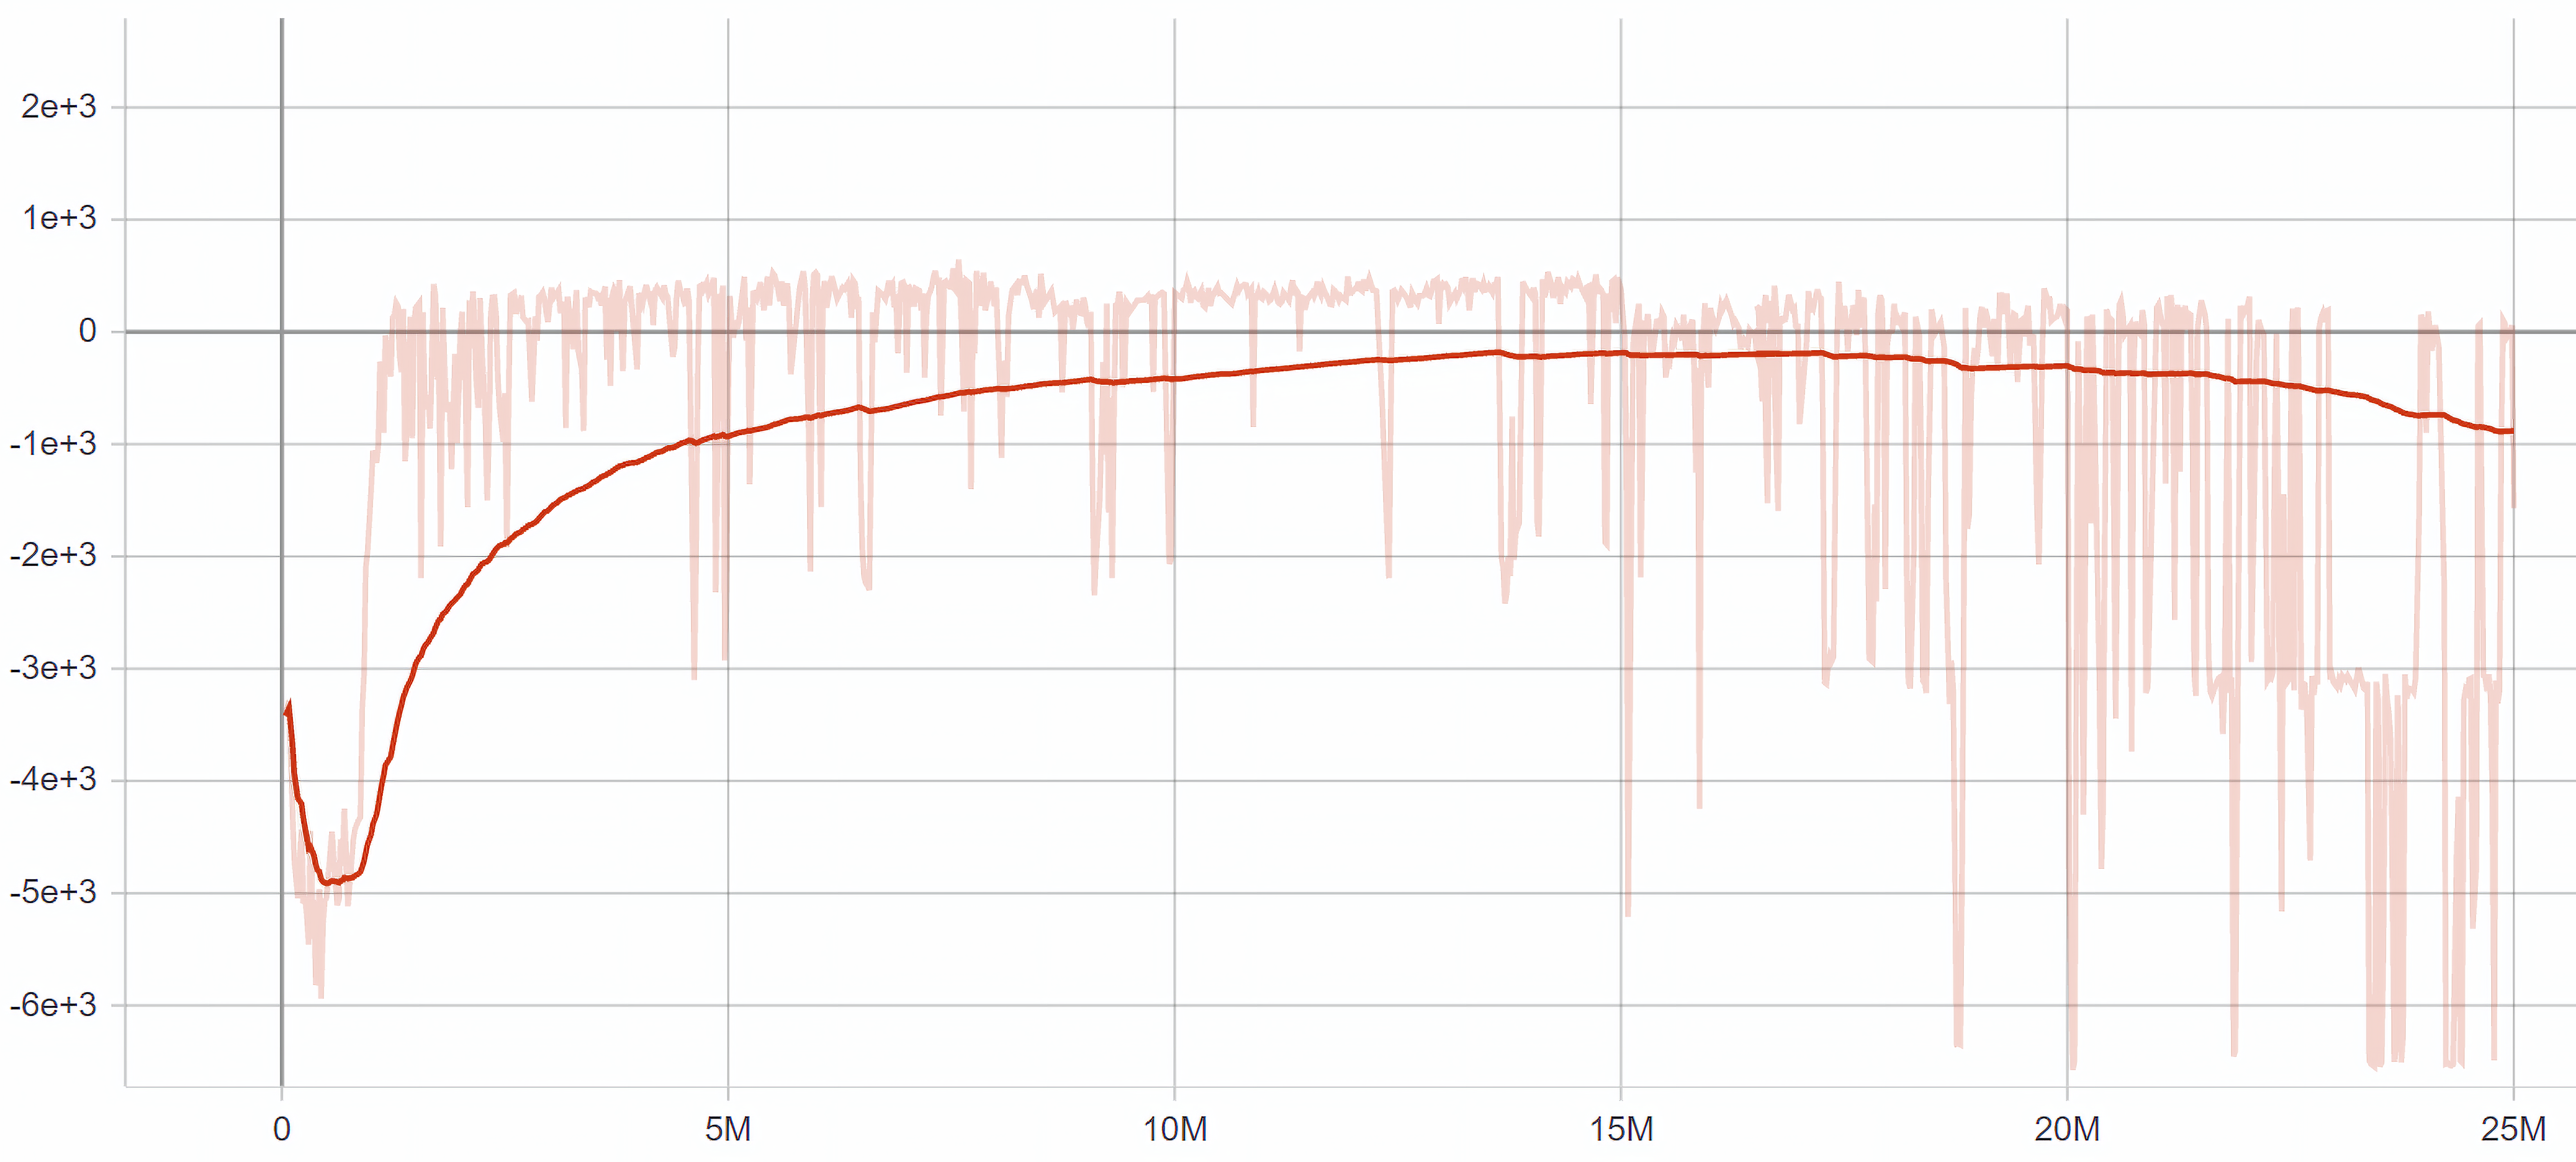
\includegraphics[scale=0.4]{Figures/Tensorboard4.PNG}
    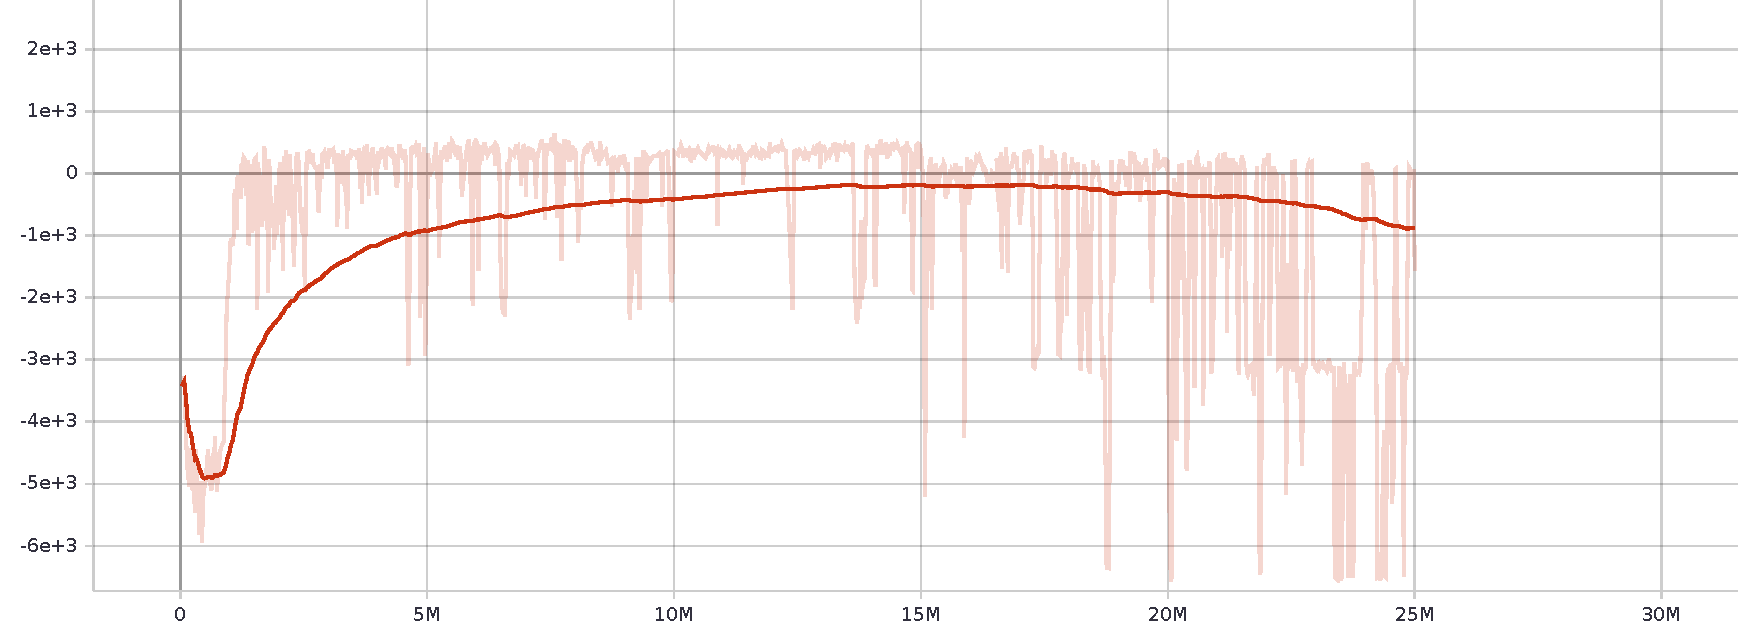
\includegraphics[width=1\linewidth]{Figures/ECumR_compressed.pdf}
    \caption{Mean Cumulative Reward vs Training Steps for the Multi-Agent System}
\end{figure}
\end{comment}


\begin{figure}
    \centering
    %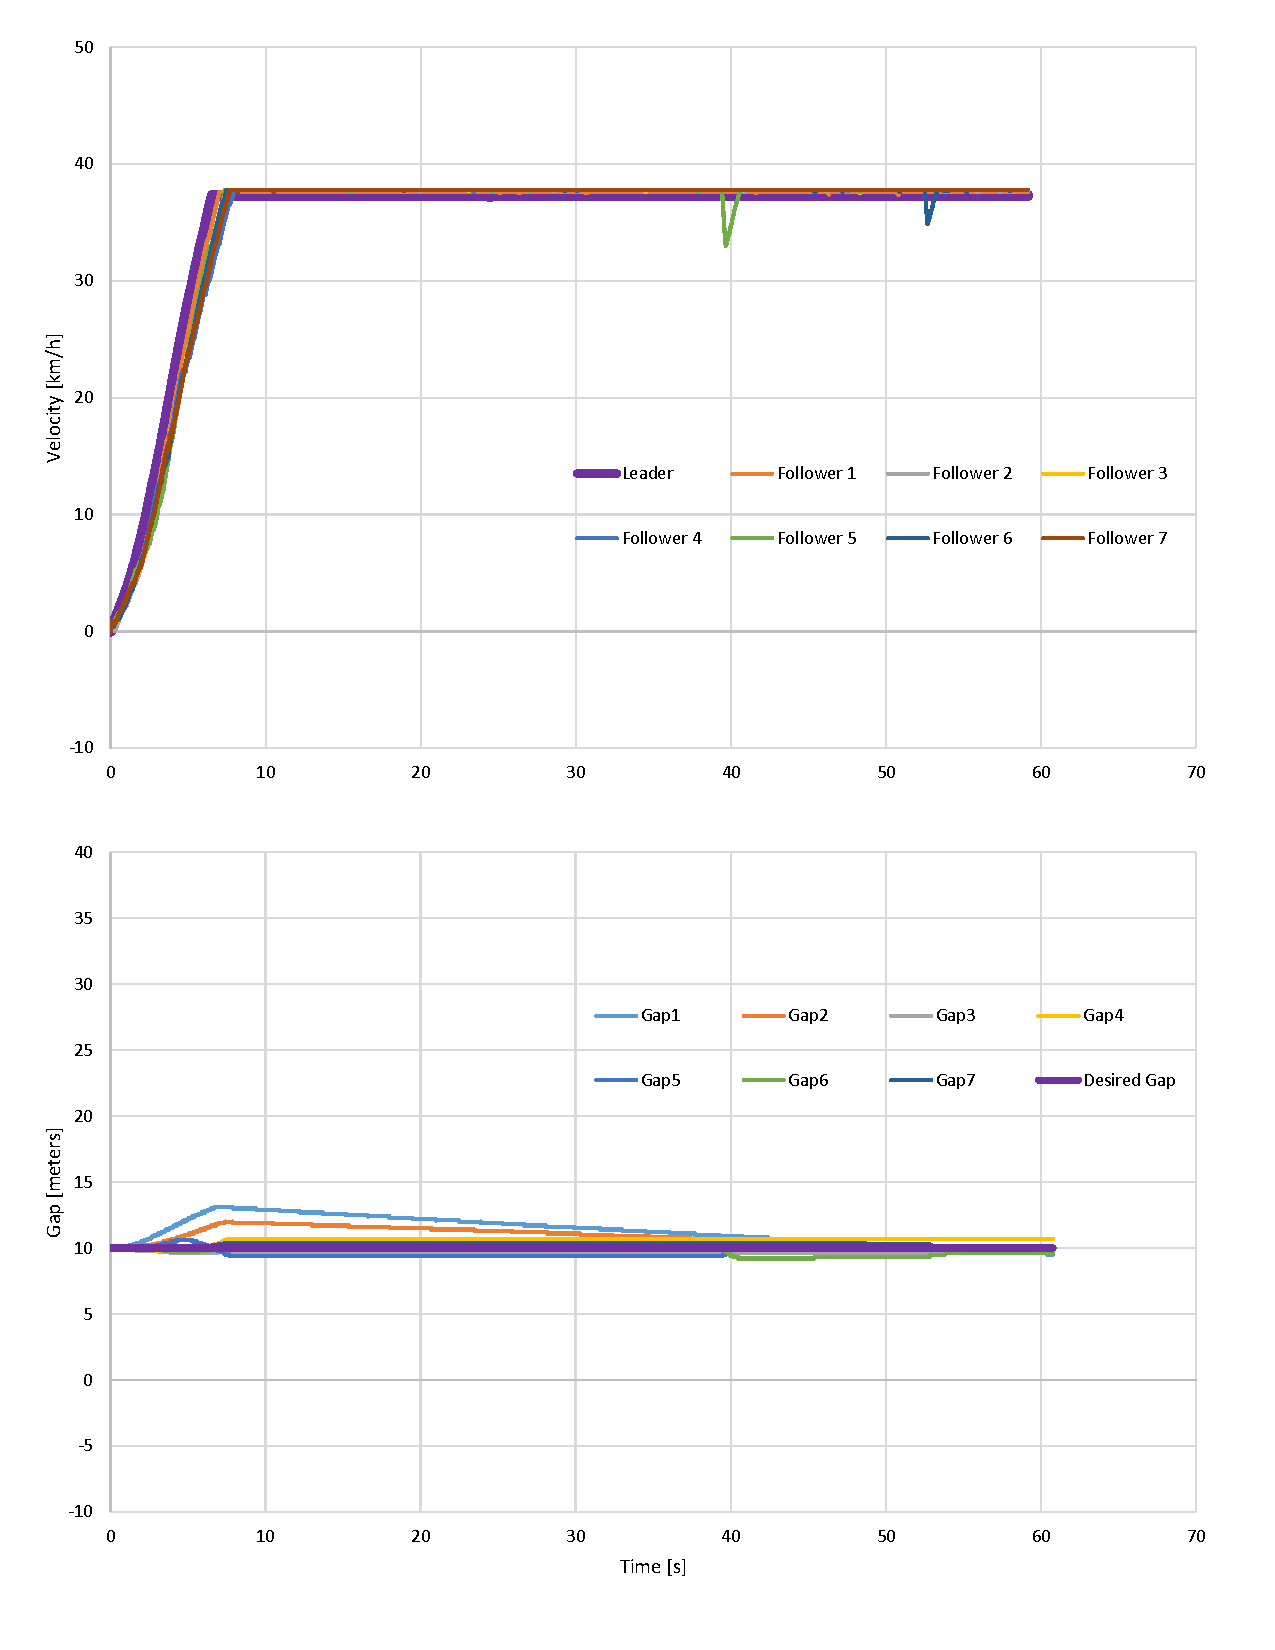
\includegraphics[width=1\linewidth]{Figures/EXP17_compressed.pdf}
    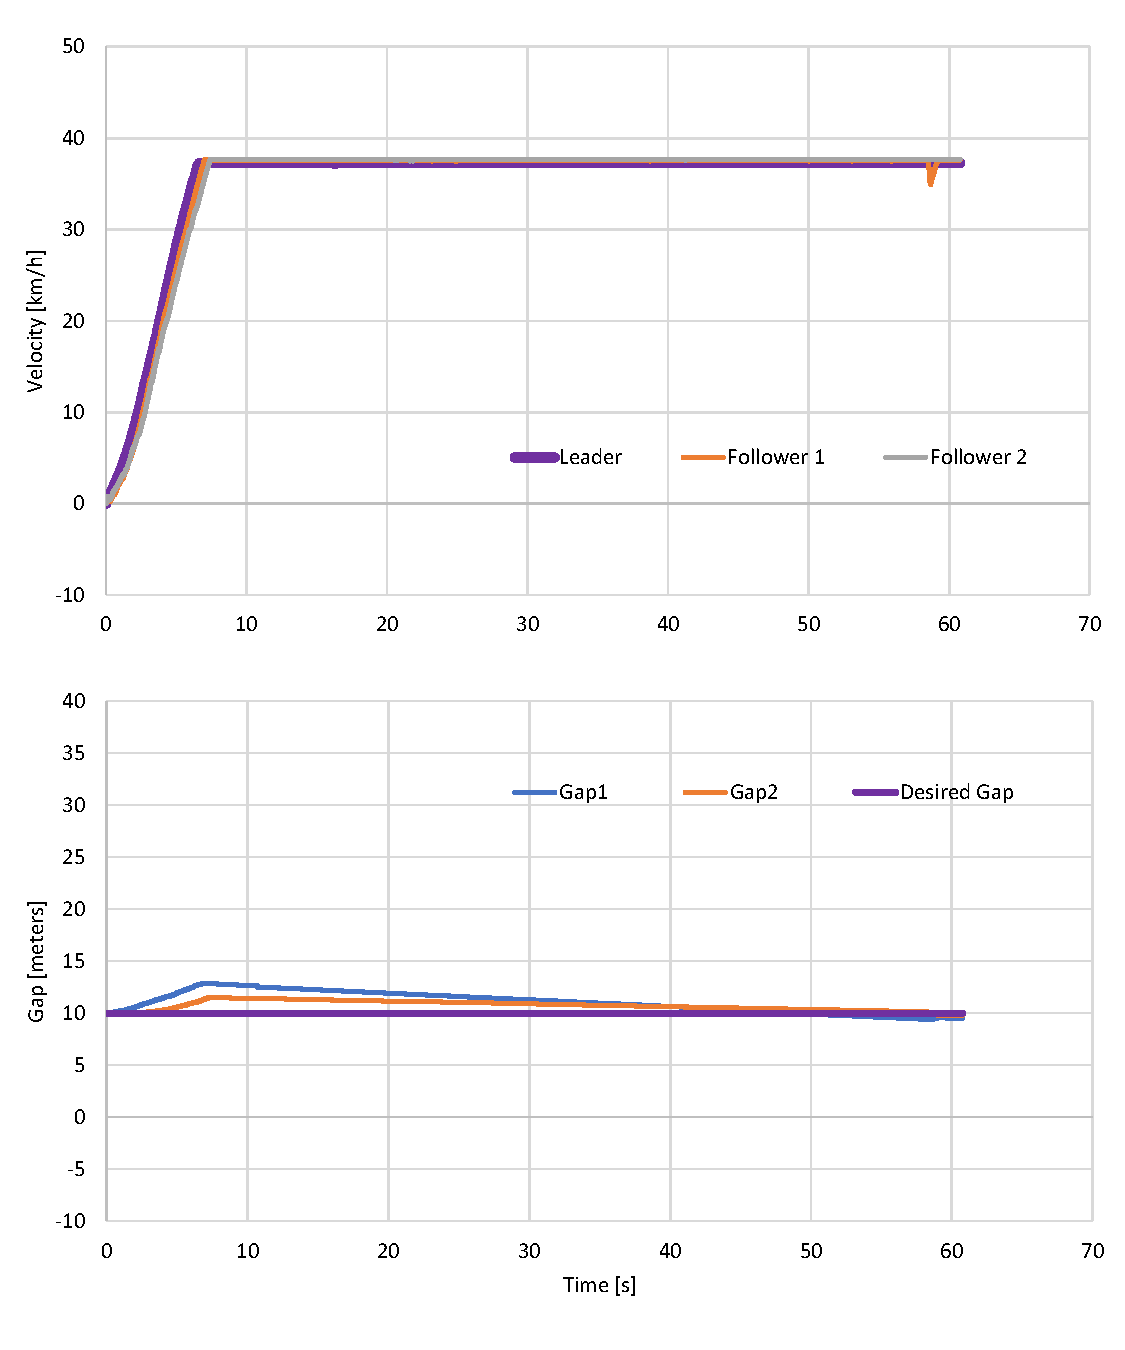
\includegraphics[width=1\linewidth]{Figures/3VGraphs3.pdf}
    %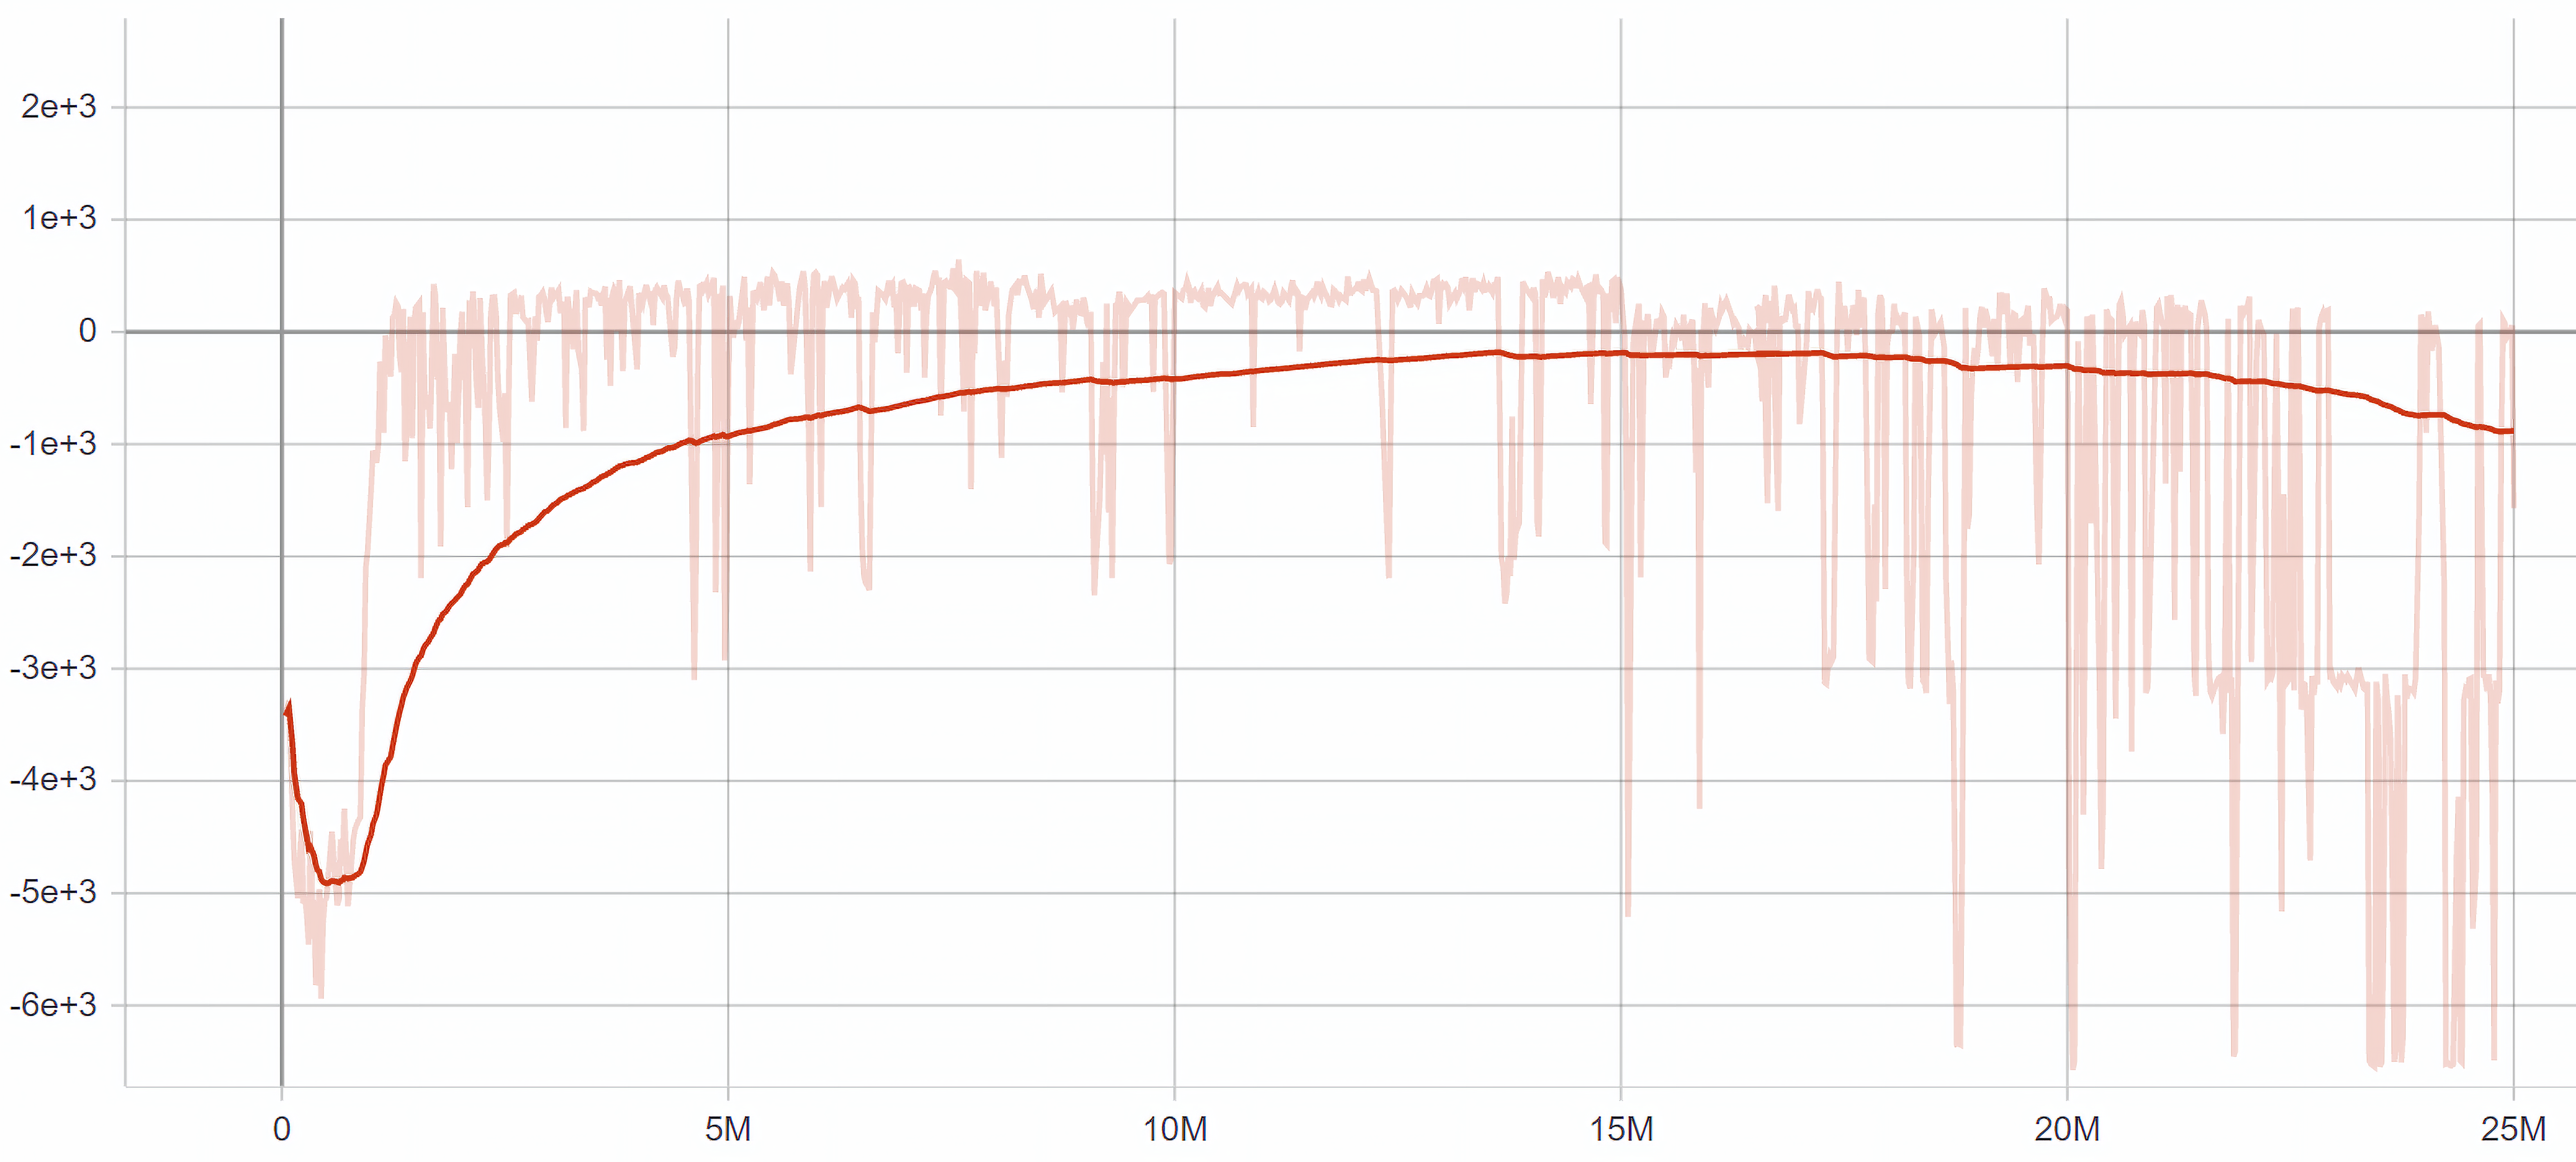
\includegraphics[scale=0.4]{Figures/Tensorboard4.PNG}
    \caption{Gap Error and Velocity Tracking of the 3 vehicles in the platoon}
\end{figure}


\begin{figure}
    \centering
    %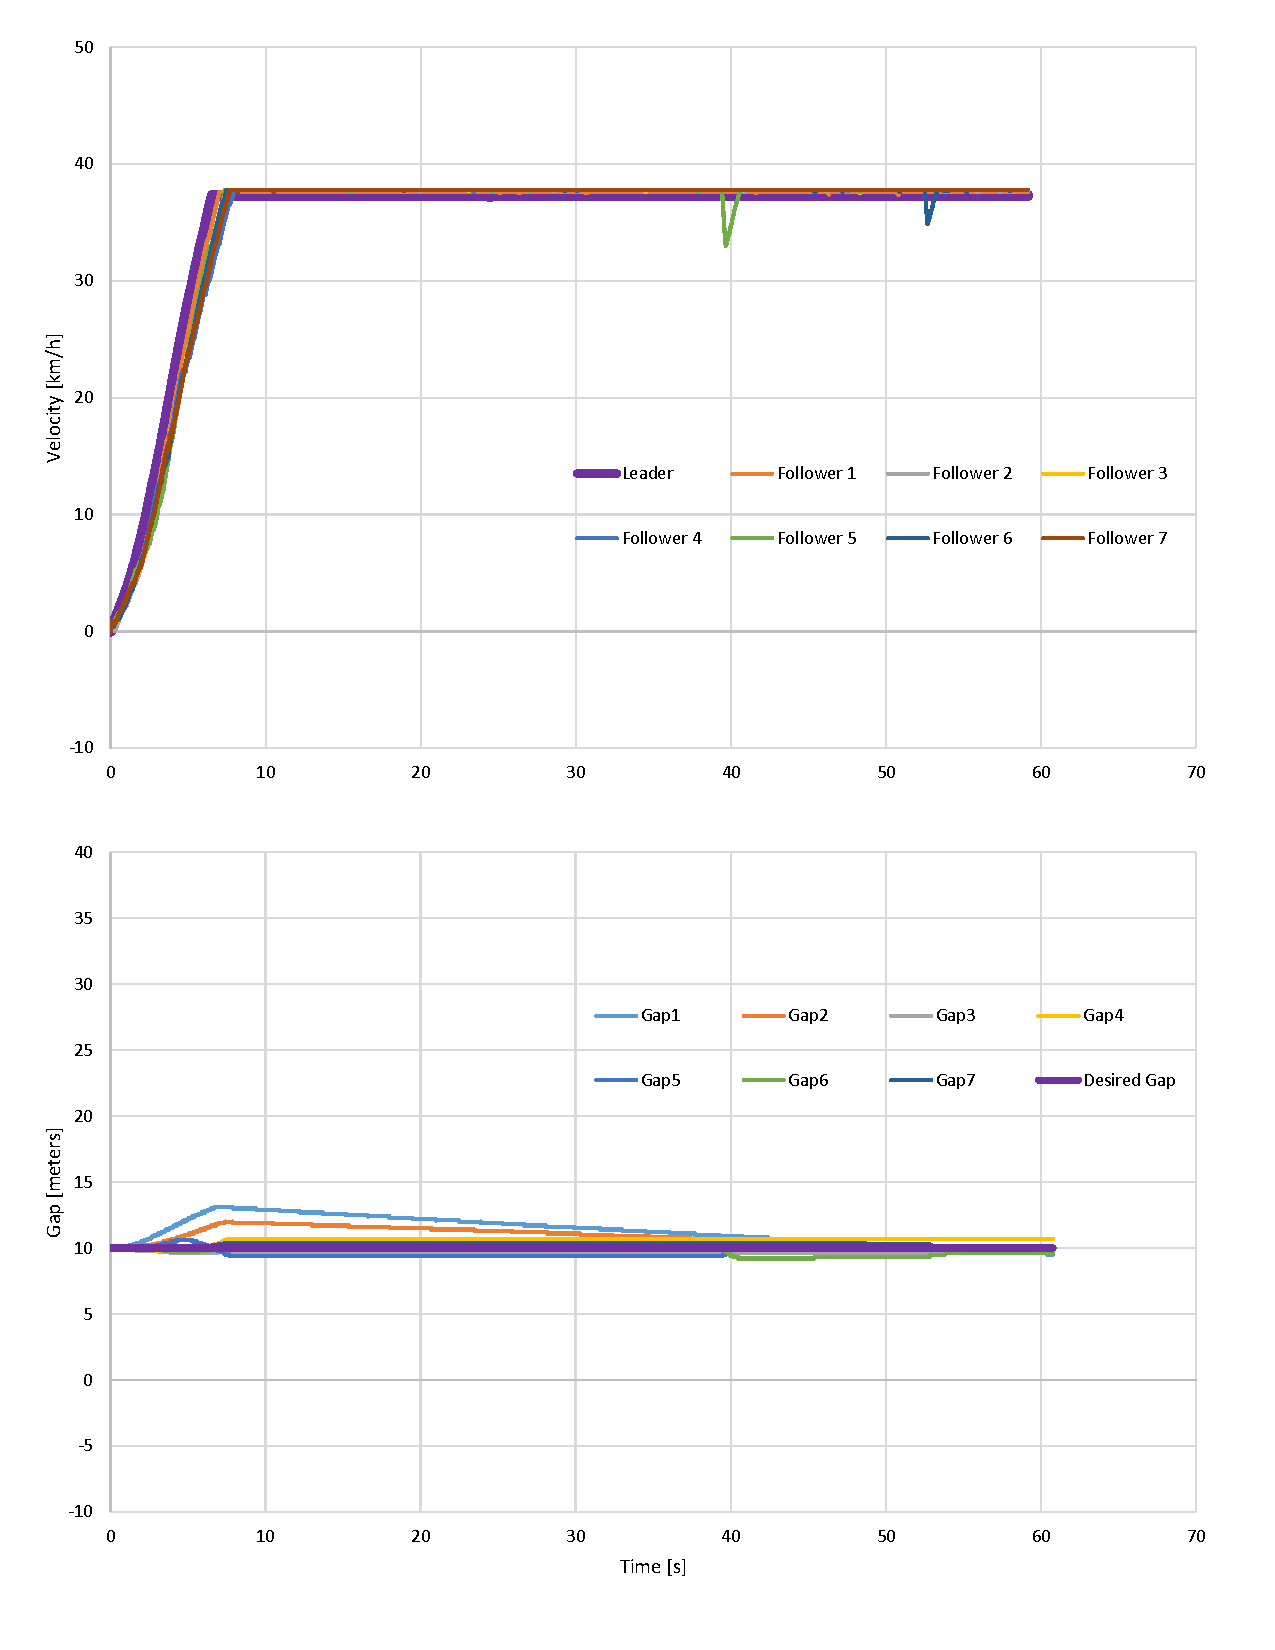
\includegraphics[width=1\linewidth]{Figures/EXP17_compressed.pdf}
    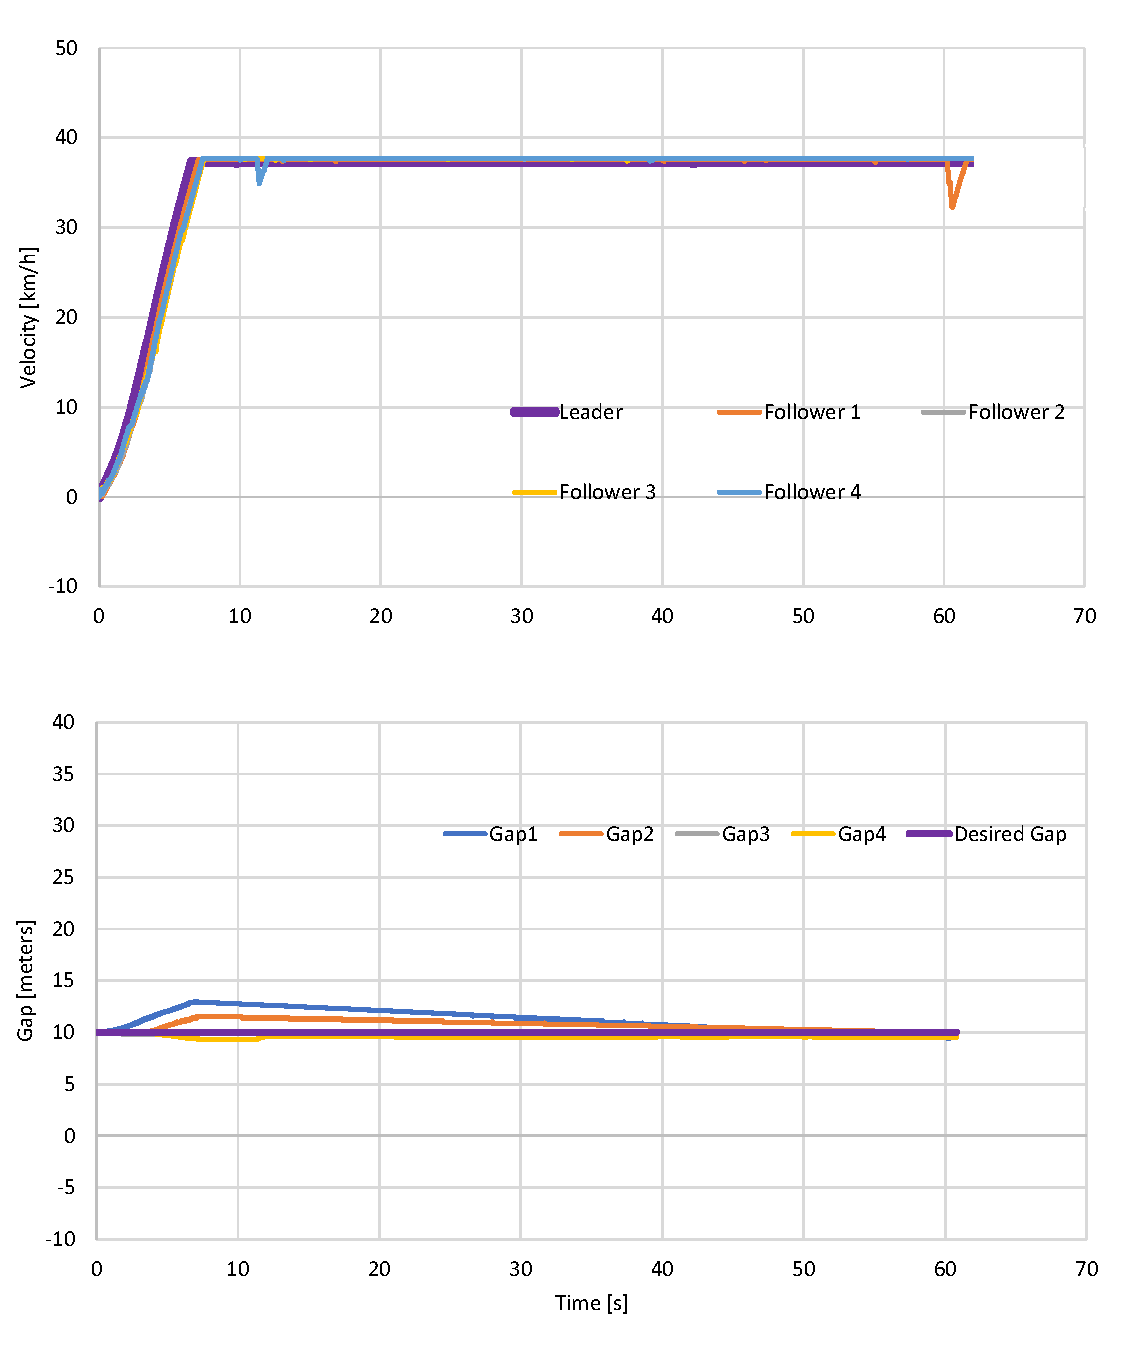
\includegraphics[width=1\linewidth]{Figures/5VGraphs3.pdf}
    %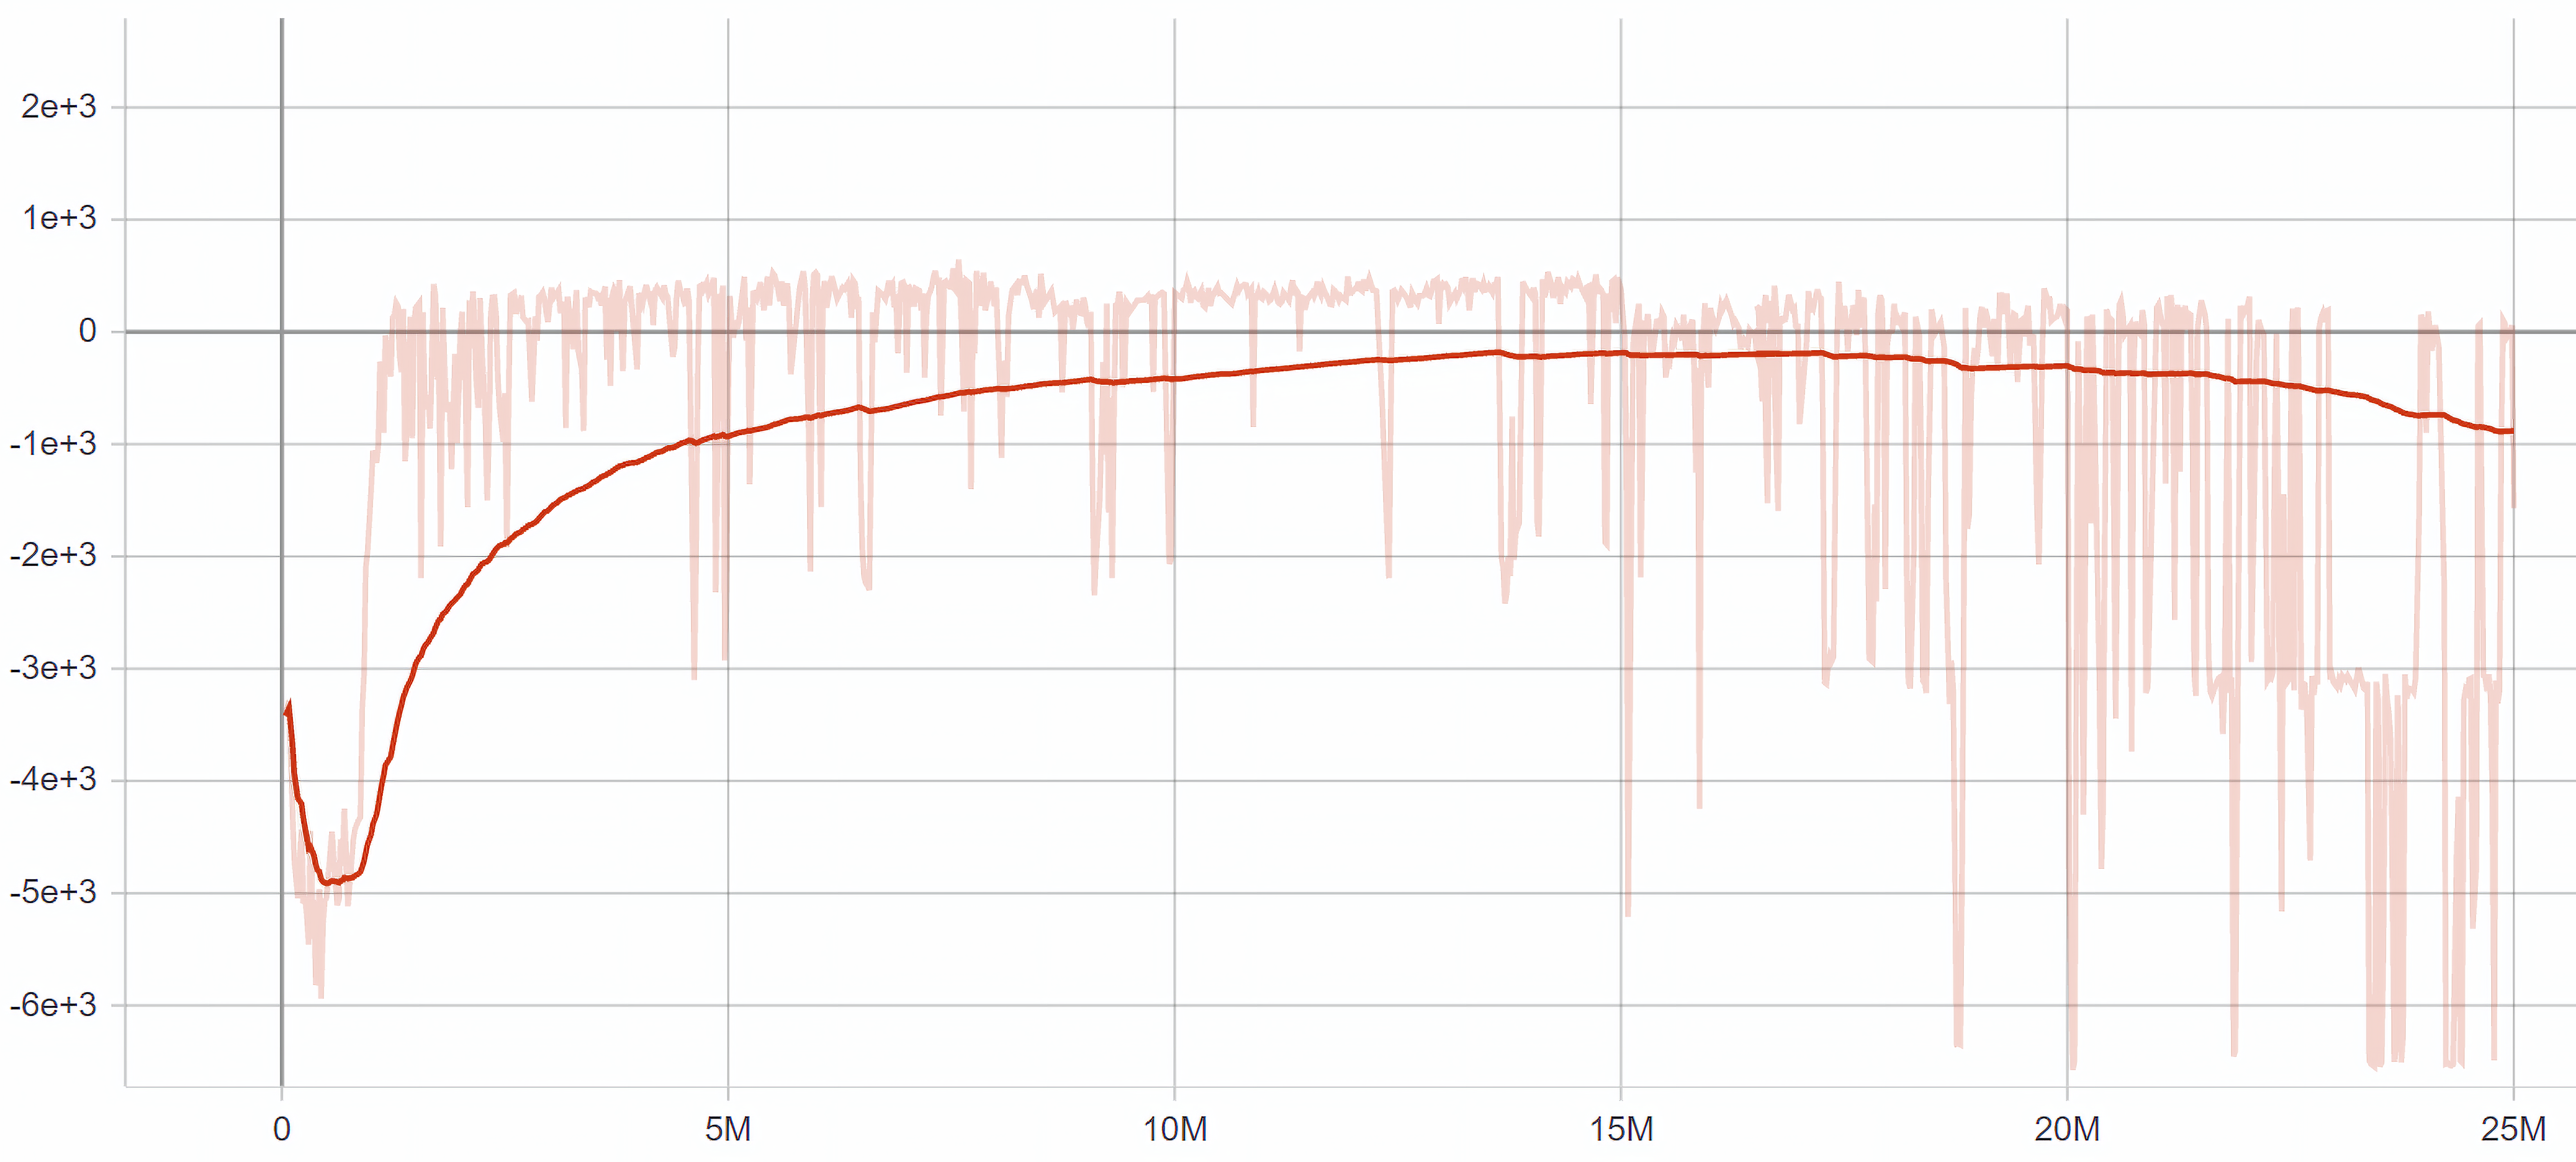
\includegraphics[scale=0.4]{Figures/Tensorboard4.PNG}
    \caption{Gap Error and Velocity Tracking of the 5 vehicles in the platoon}
\end{figure}


\begin{comment}
\begin{figure}[H]
    \centering
    %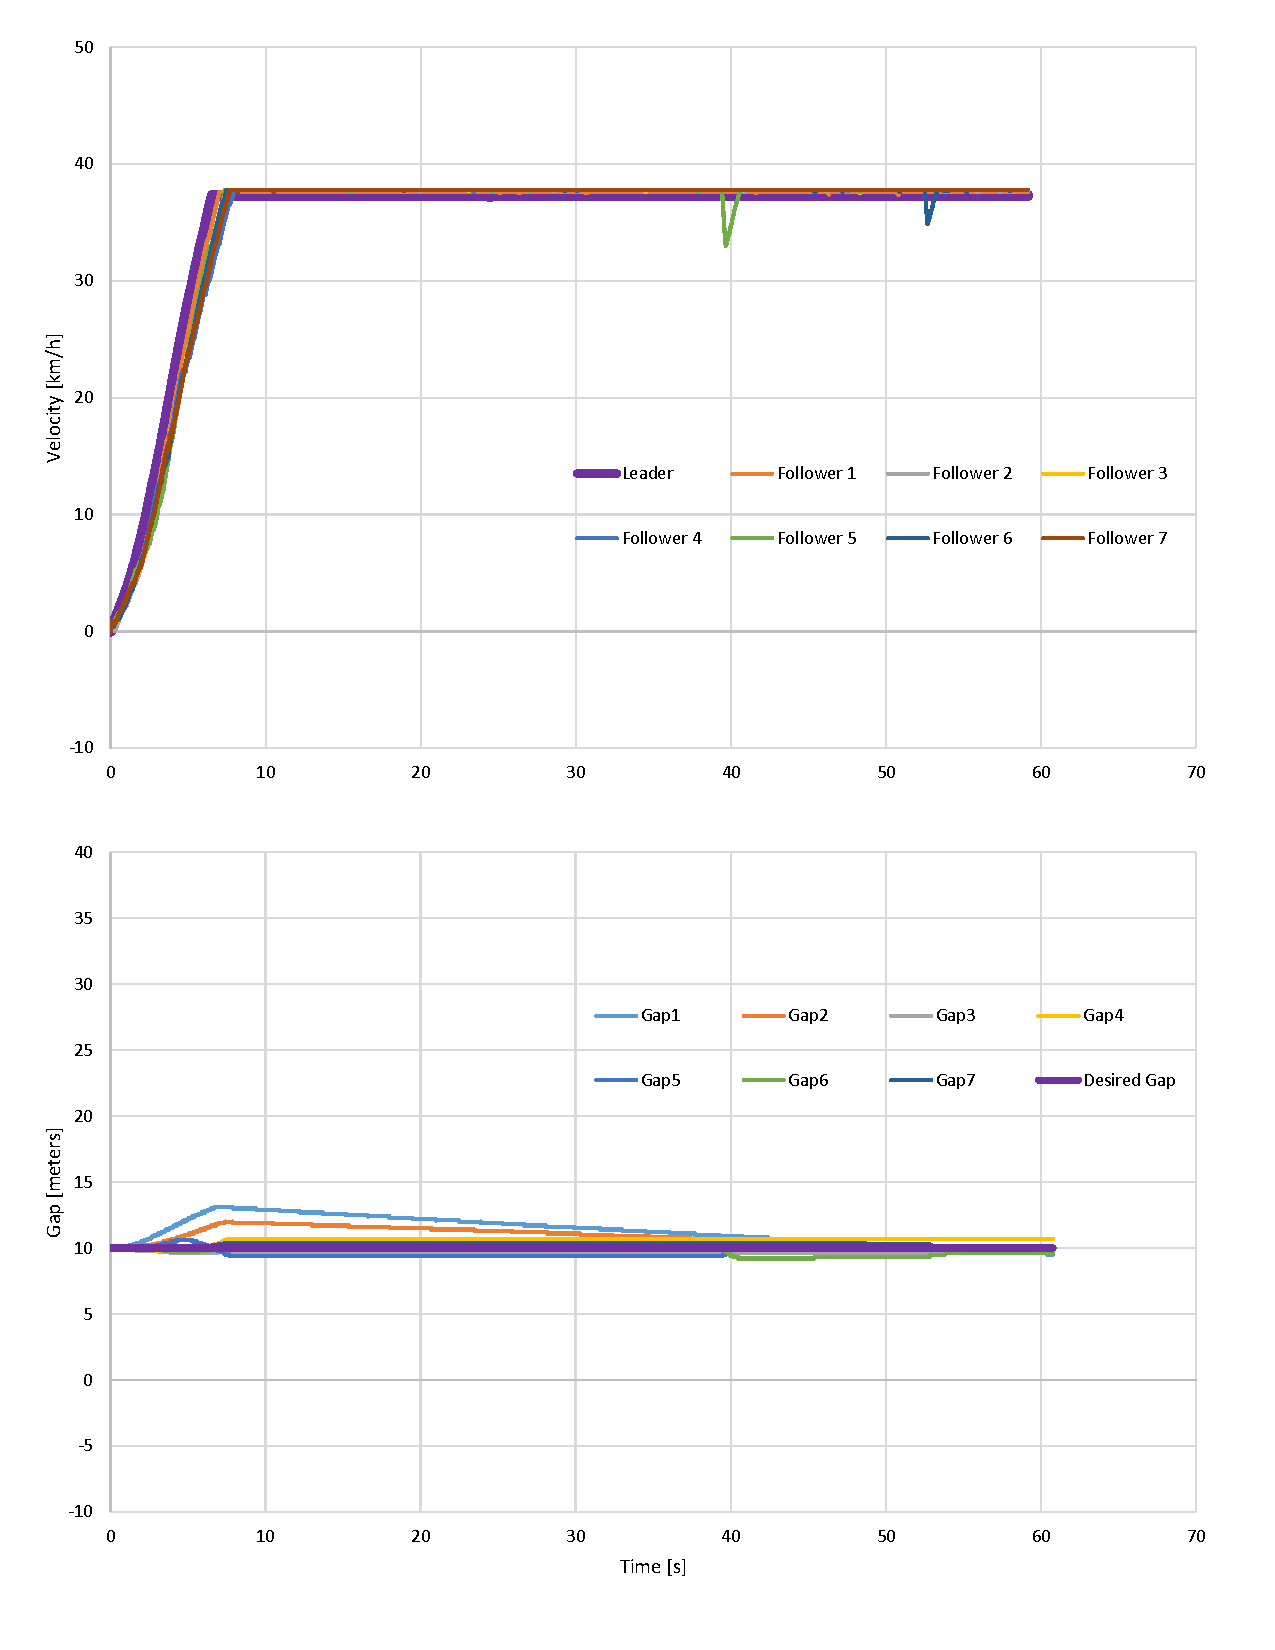
\includegraphics[width=1\linewidth]{Figures/EXP17_compressed.pdf}
    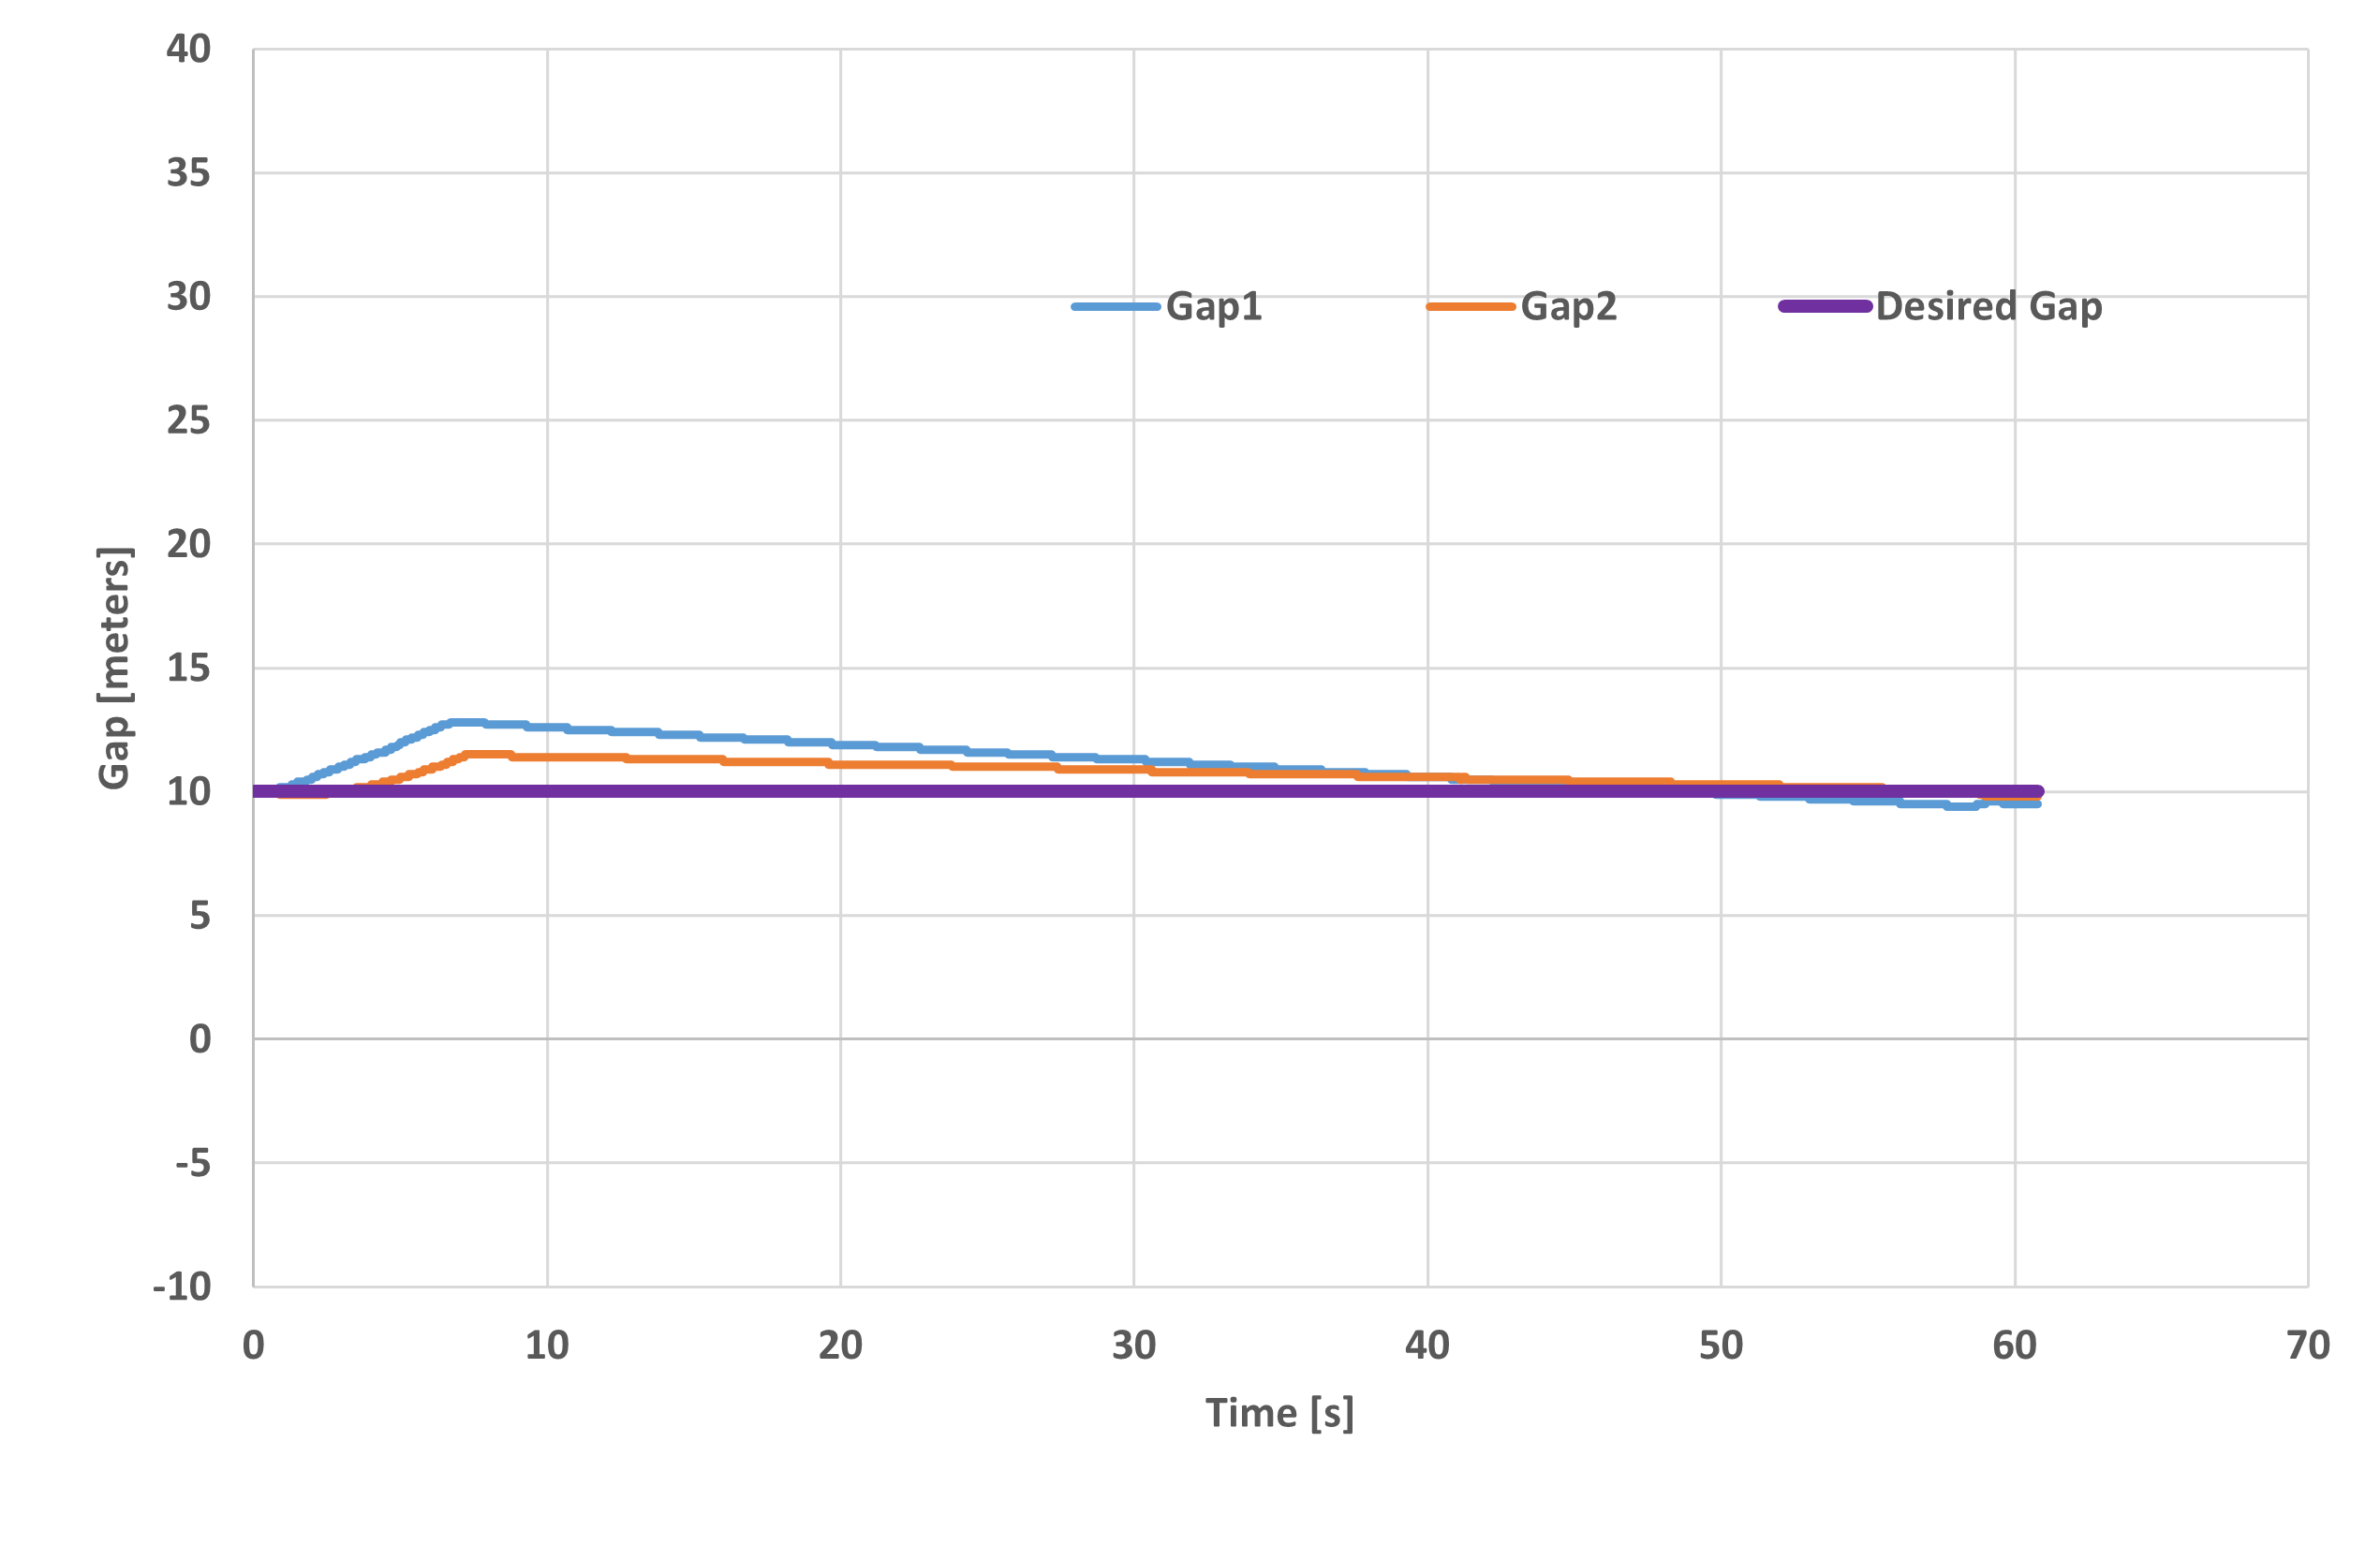
\includegraphics[width=1\linewidth]{Figures/3_vehicles_gap.png}
    %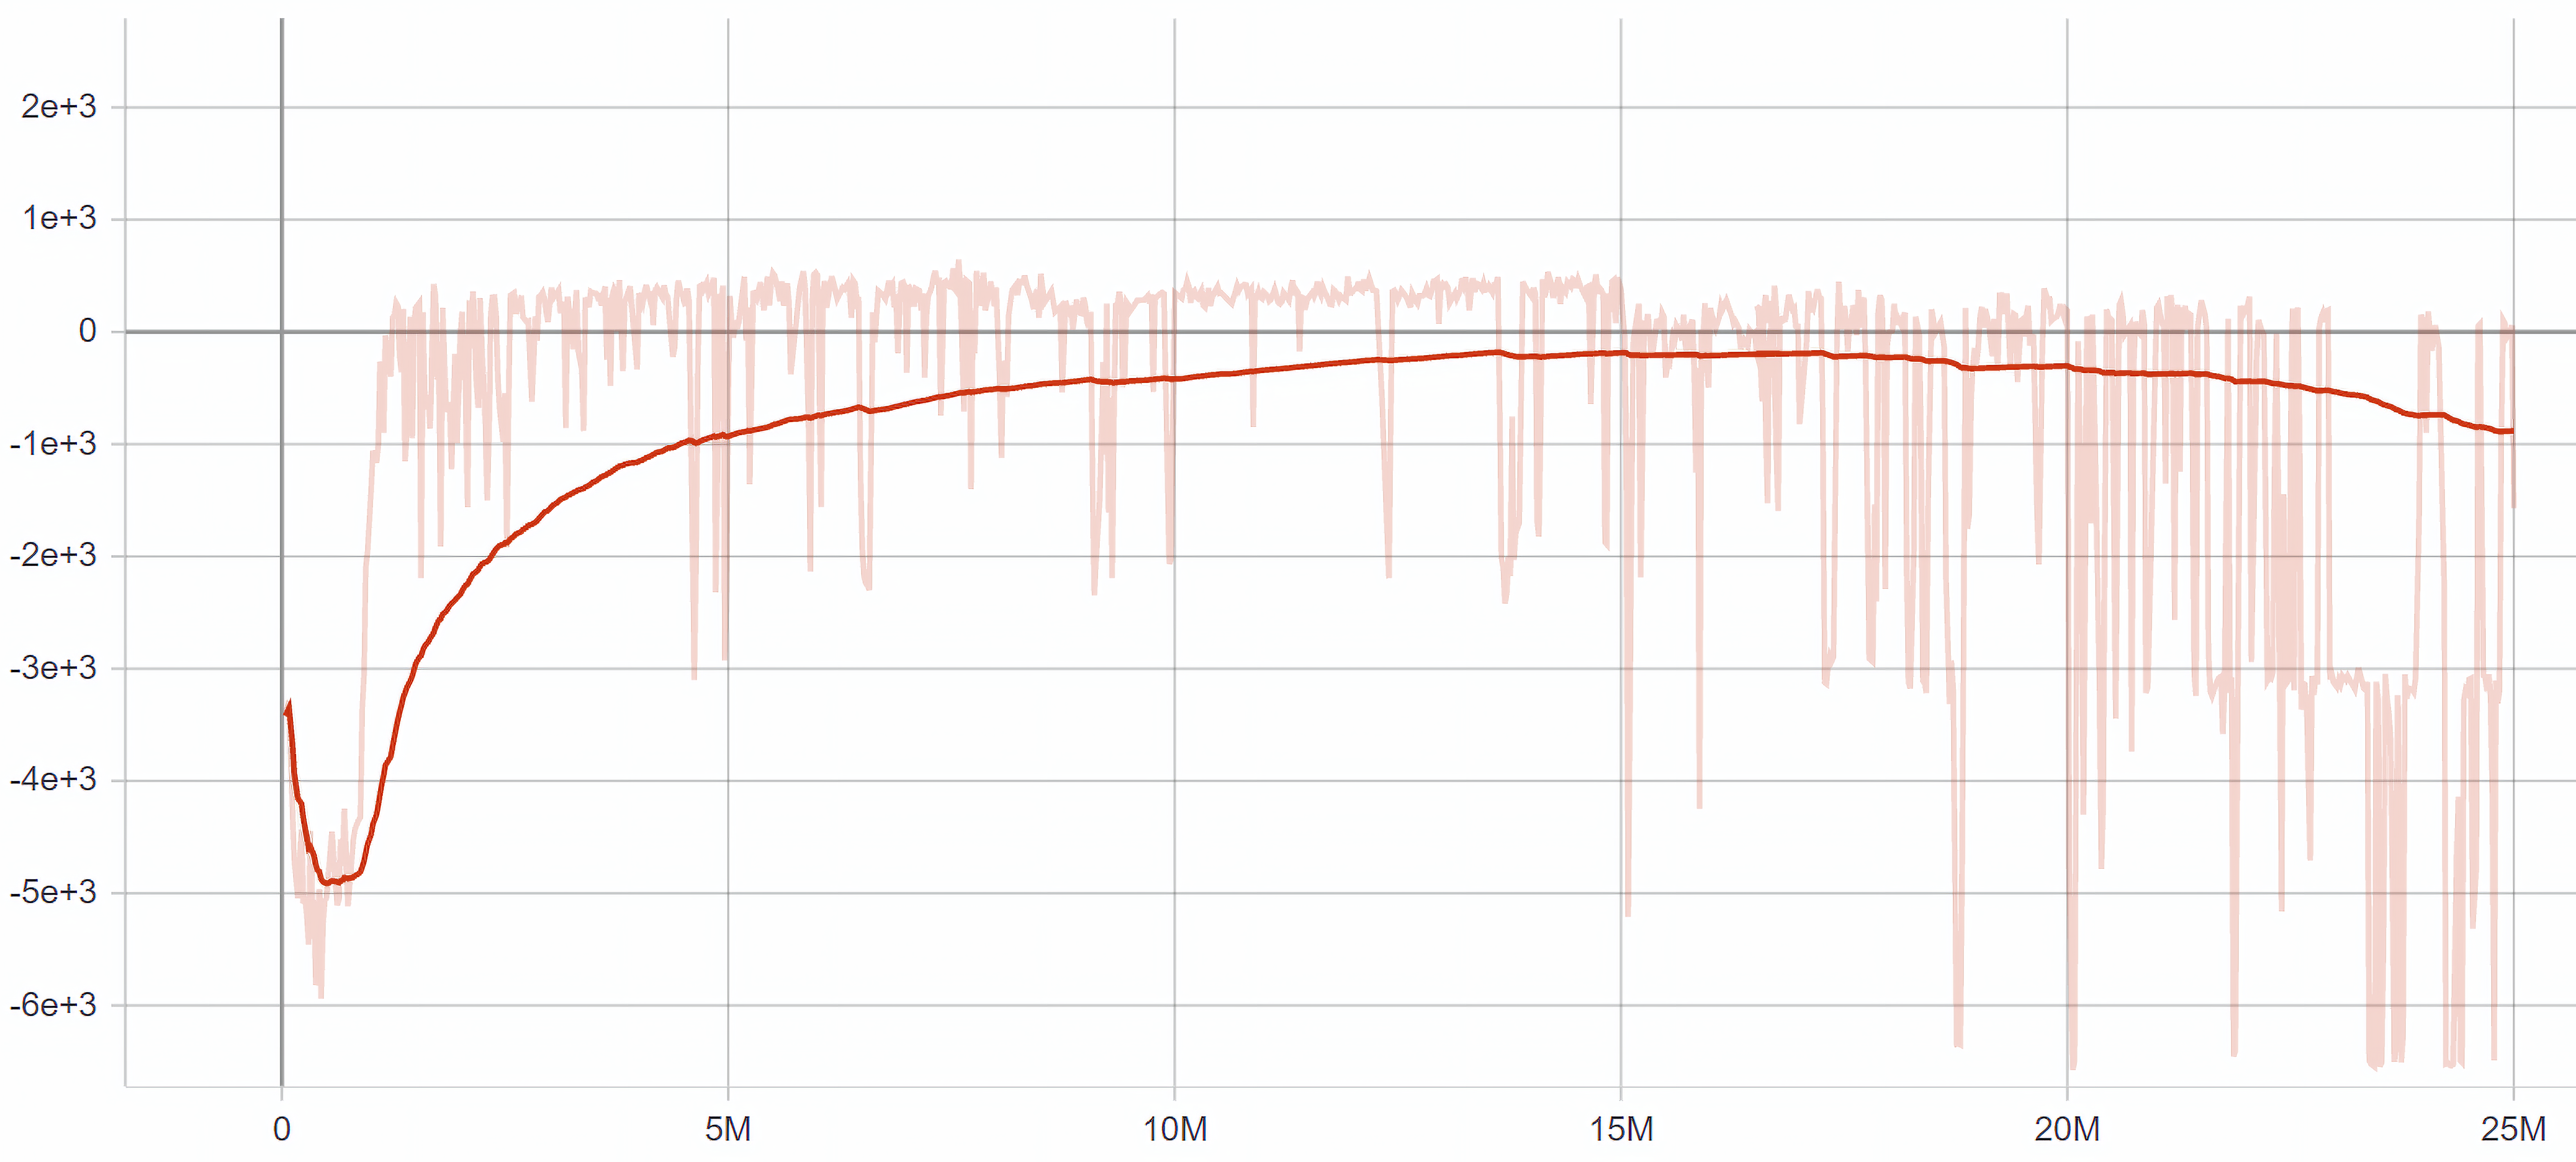
\includegraphics[scale=0.4]{Figures/Tensorboard4.PNG}
    \caption{Gap Error of 3 vehicles in the platoon}
\end{figure}

\begin{figure}[H]
    \centering
    %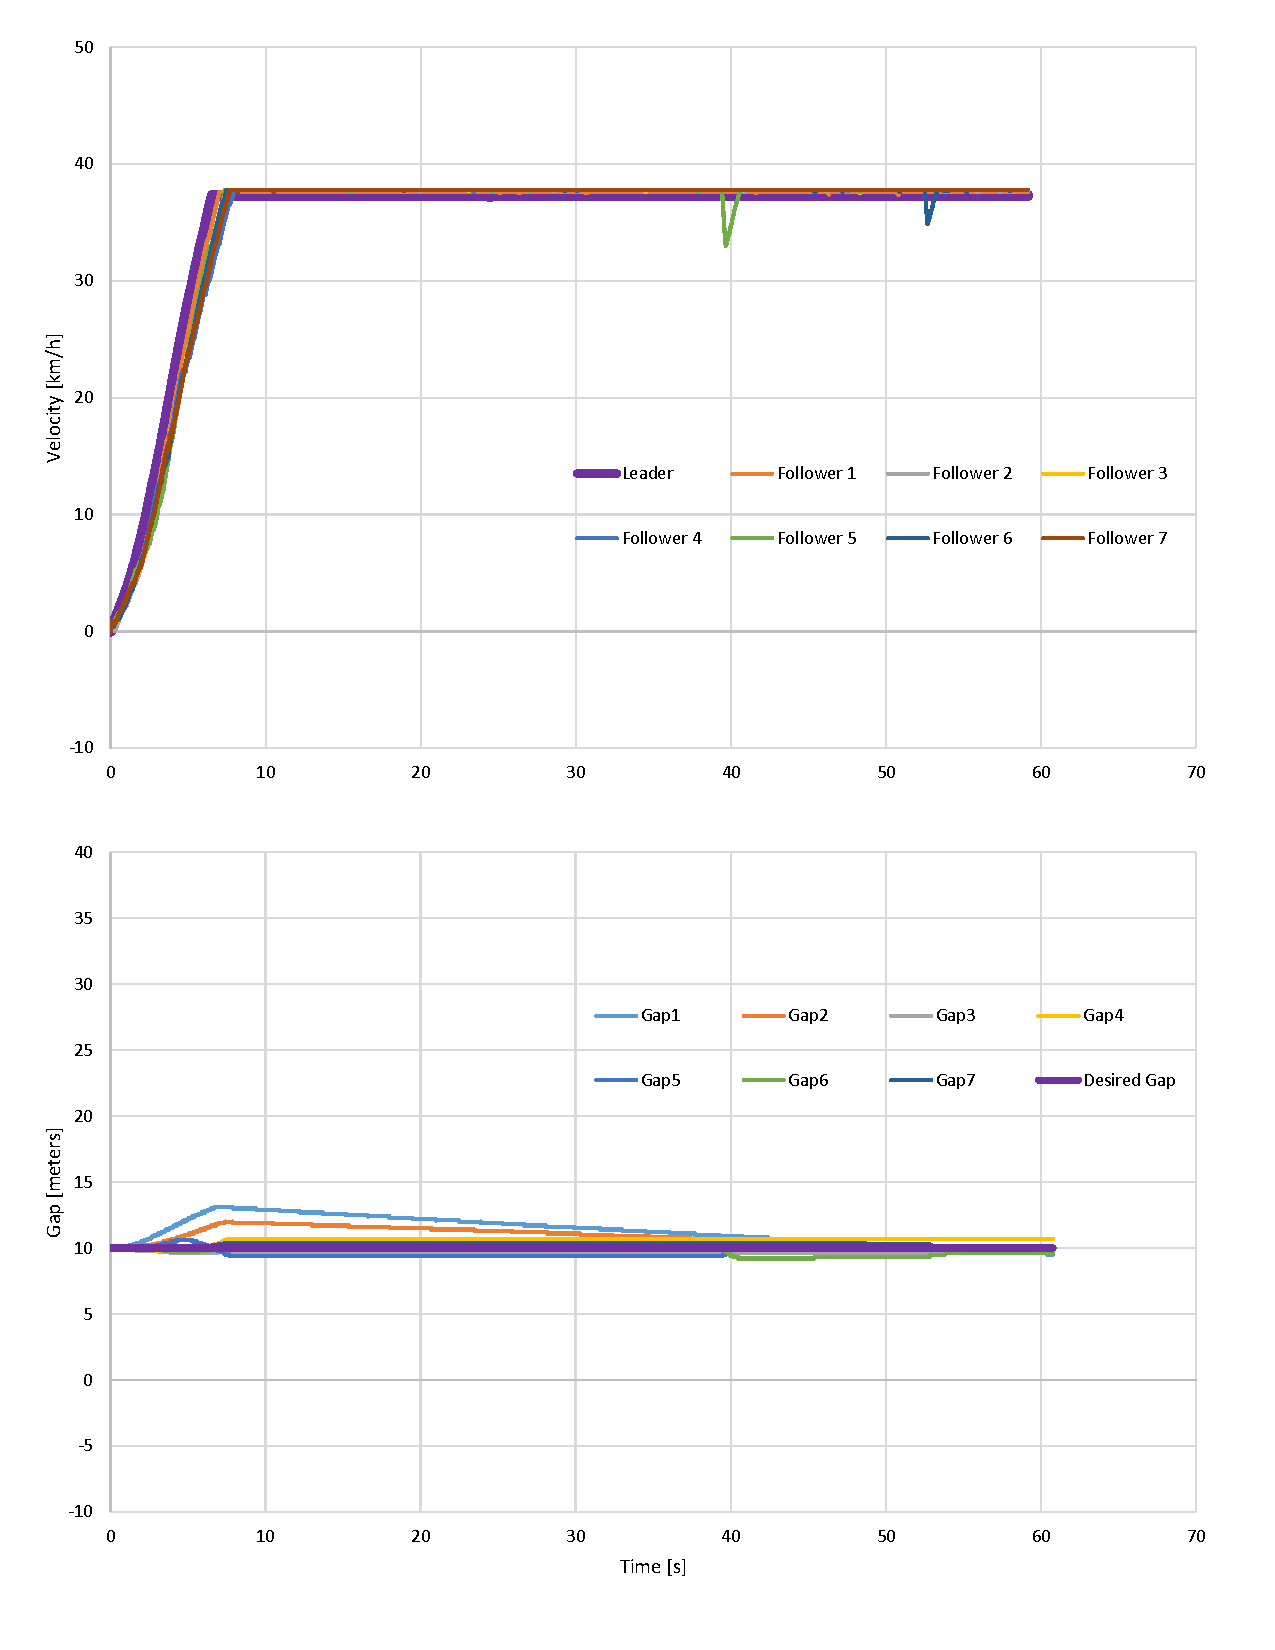
\includegraphics[width=1\linewidth]{Figures/EXP17_compressed.pdf}
    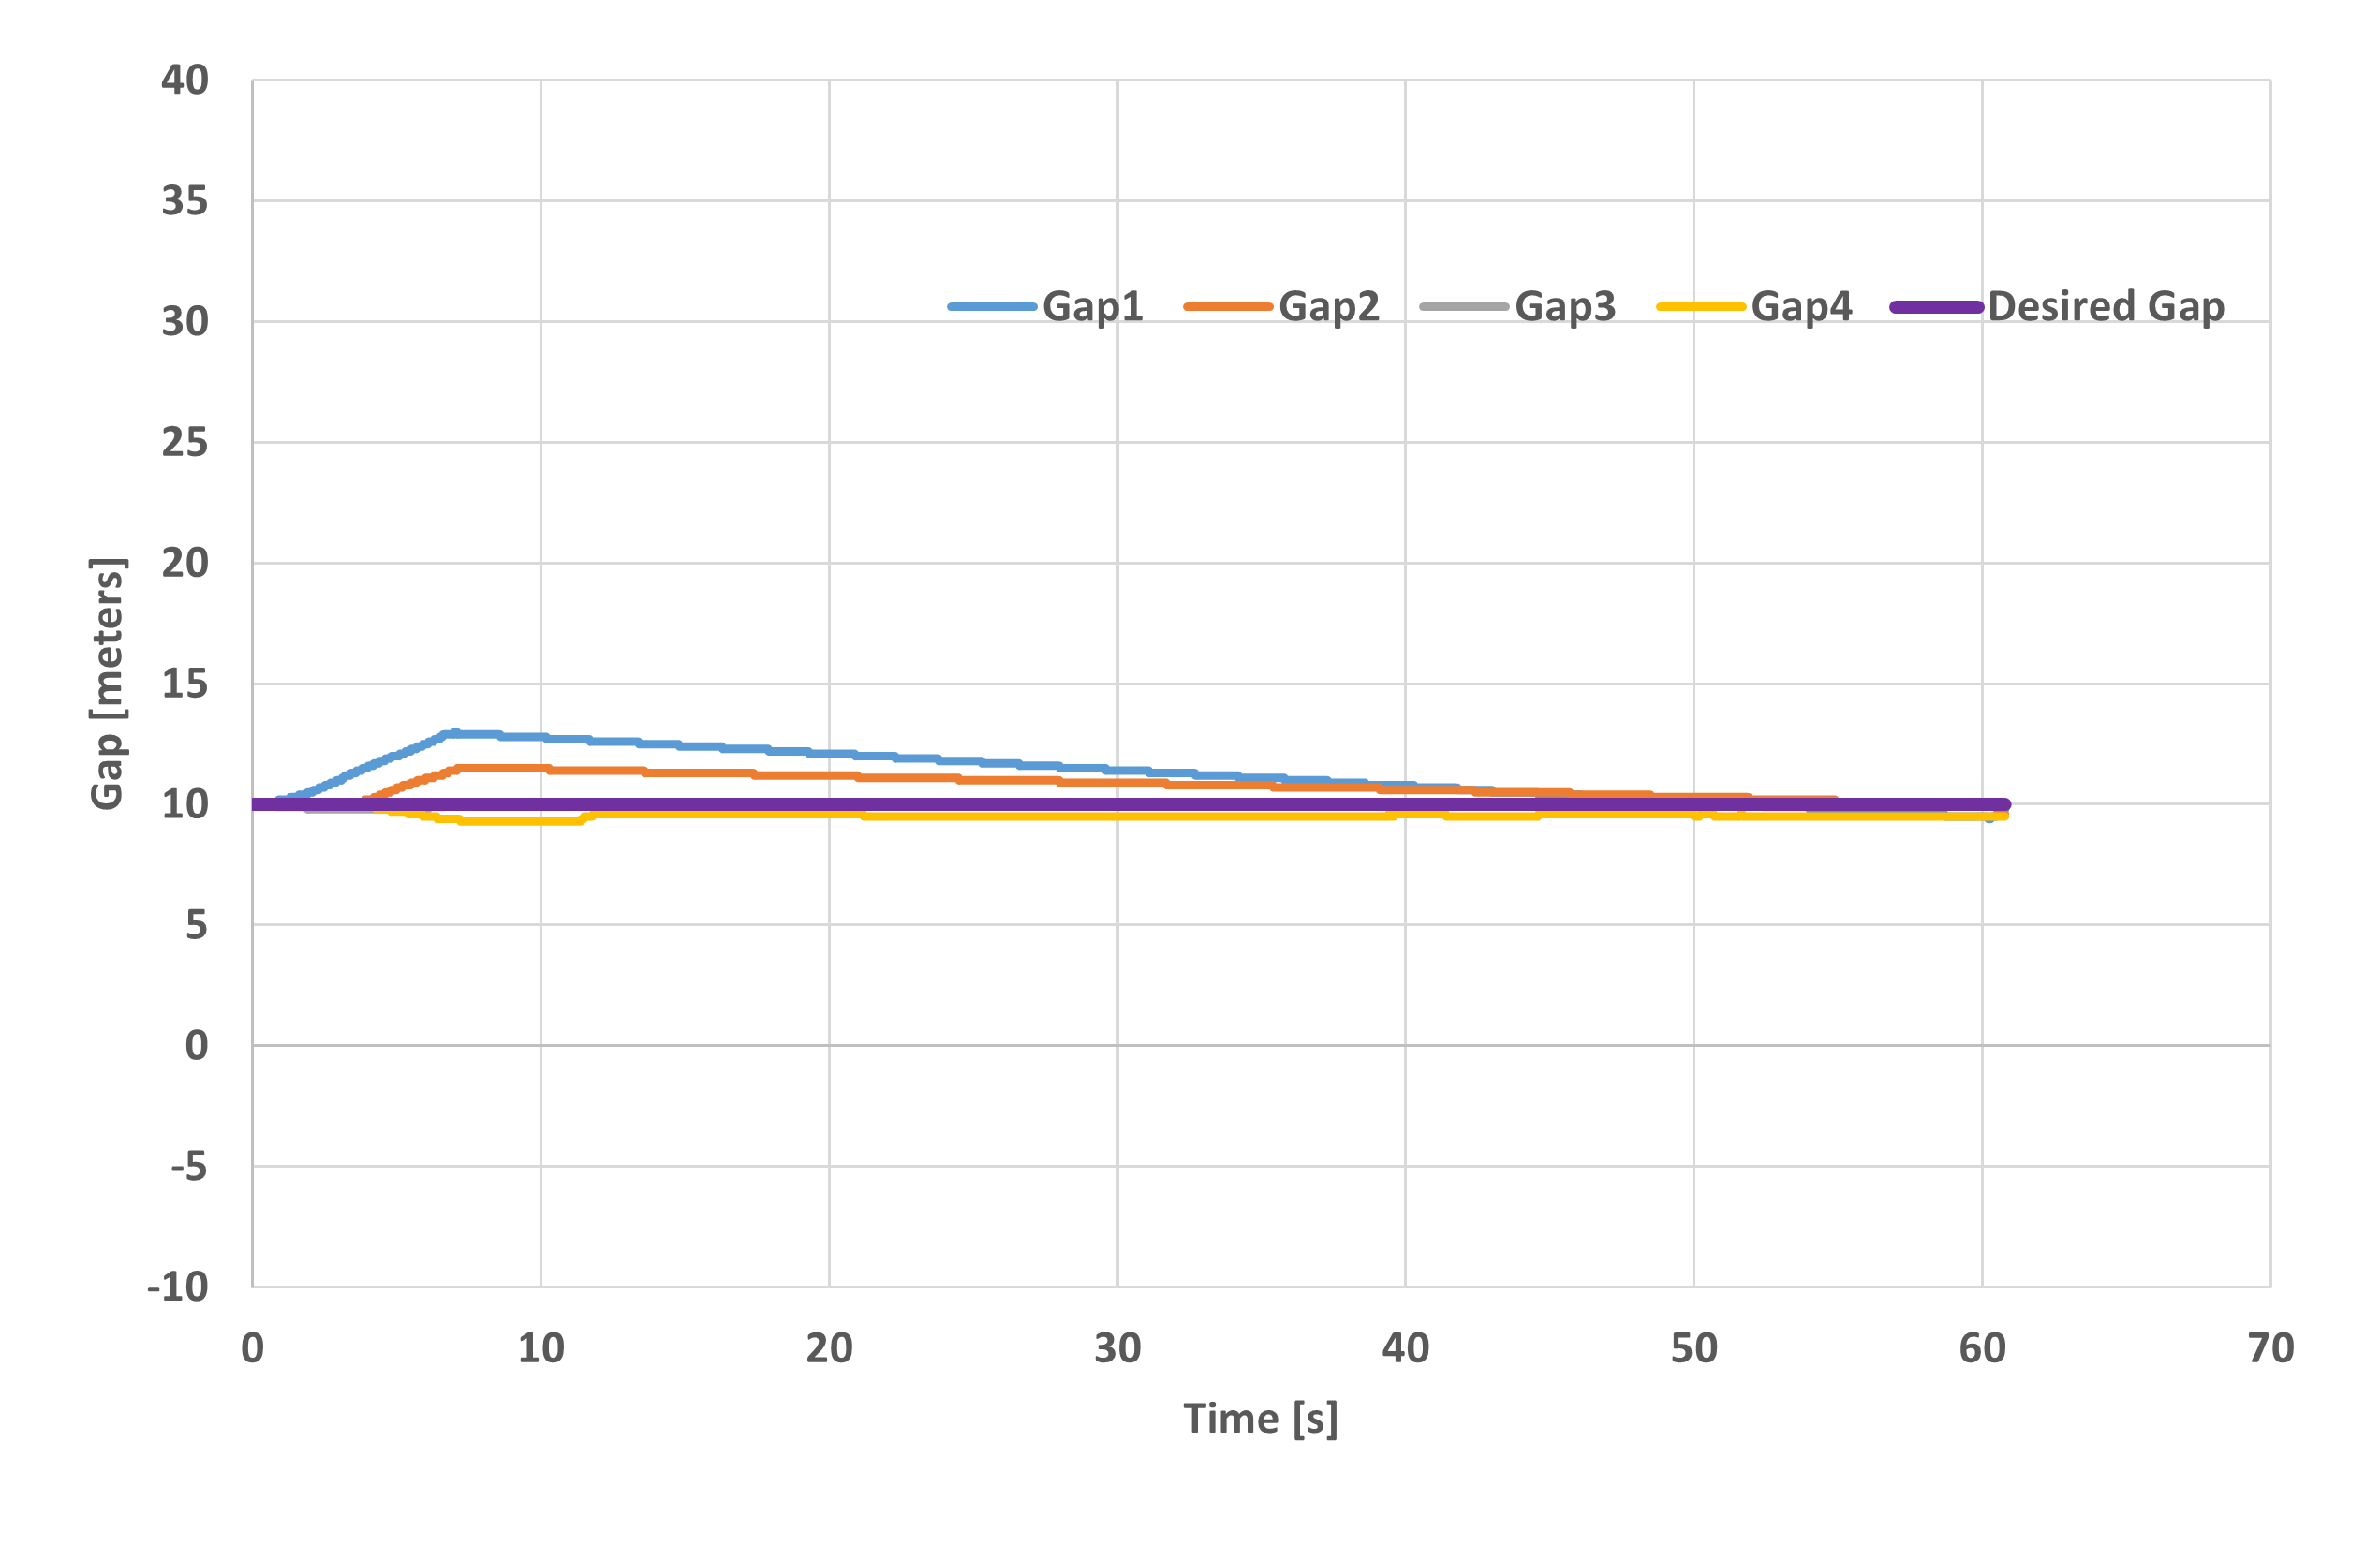
\includegraphics[width=1\linewidth]{Figures/5_vehicles_gap.png}
    %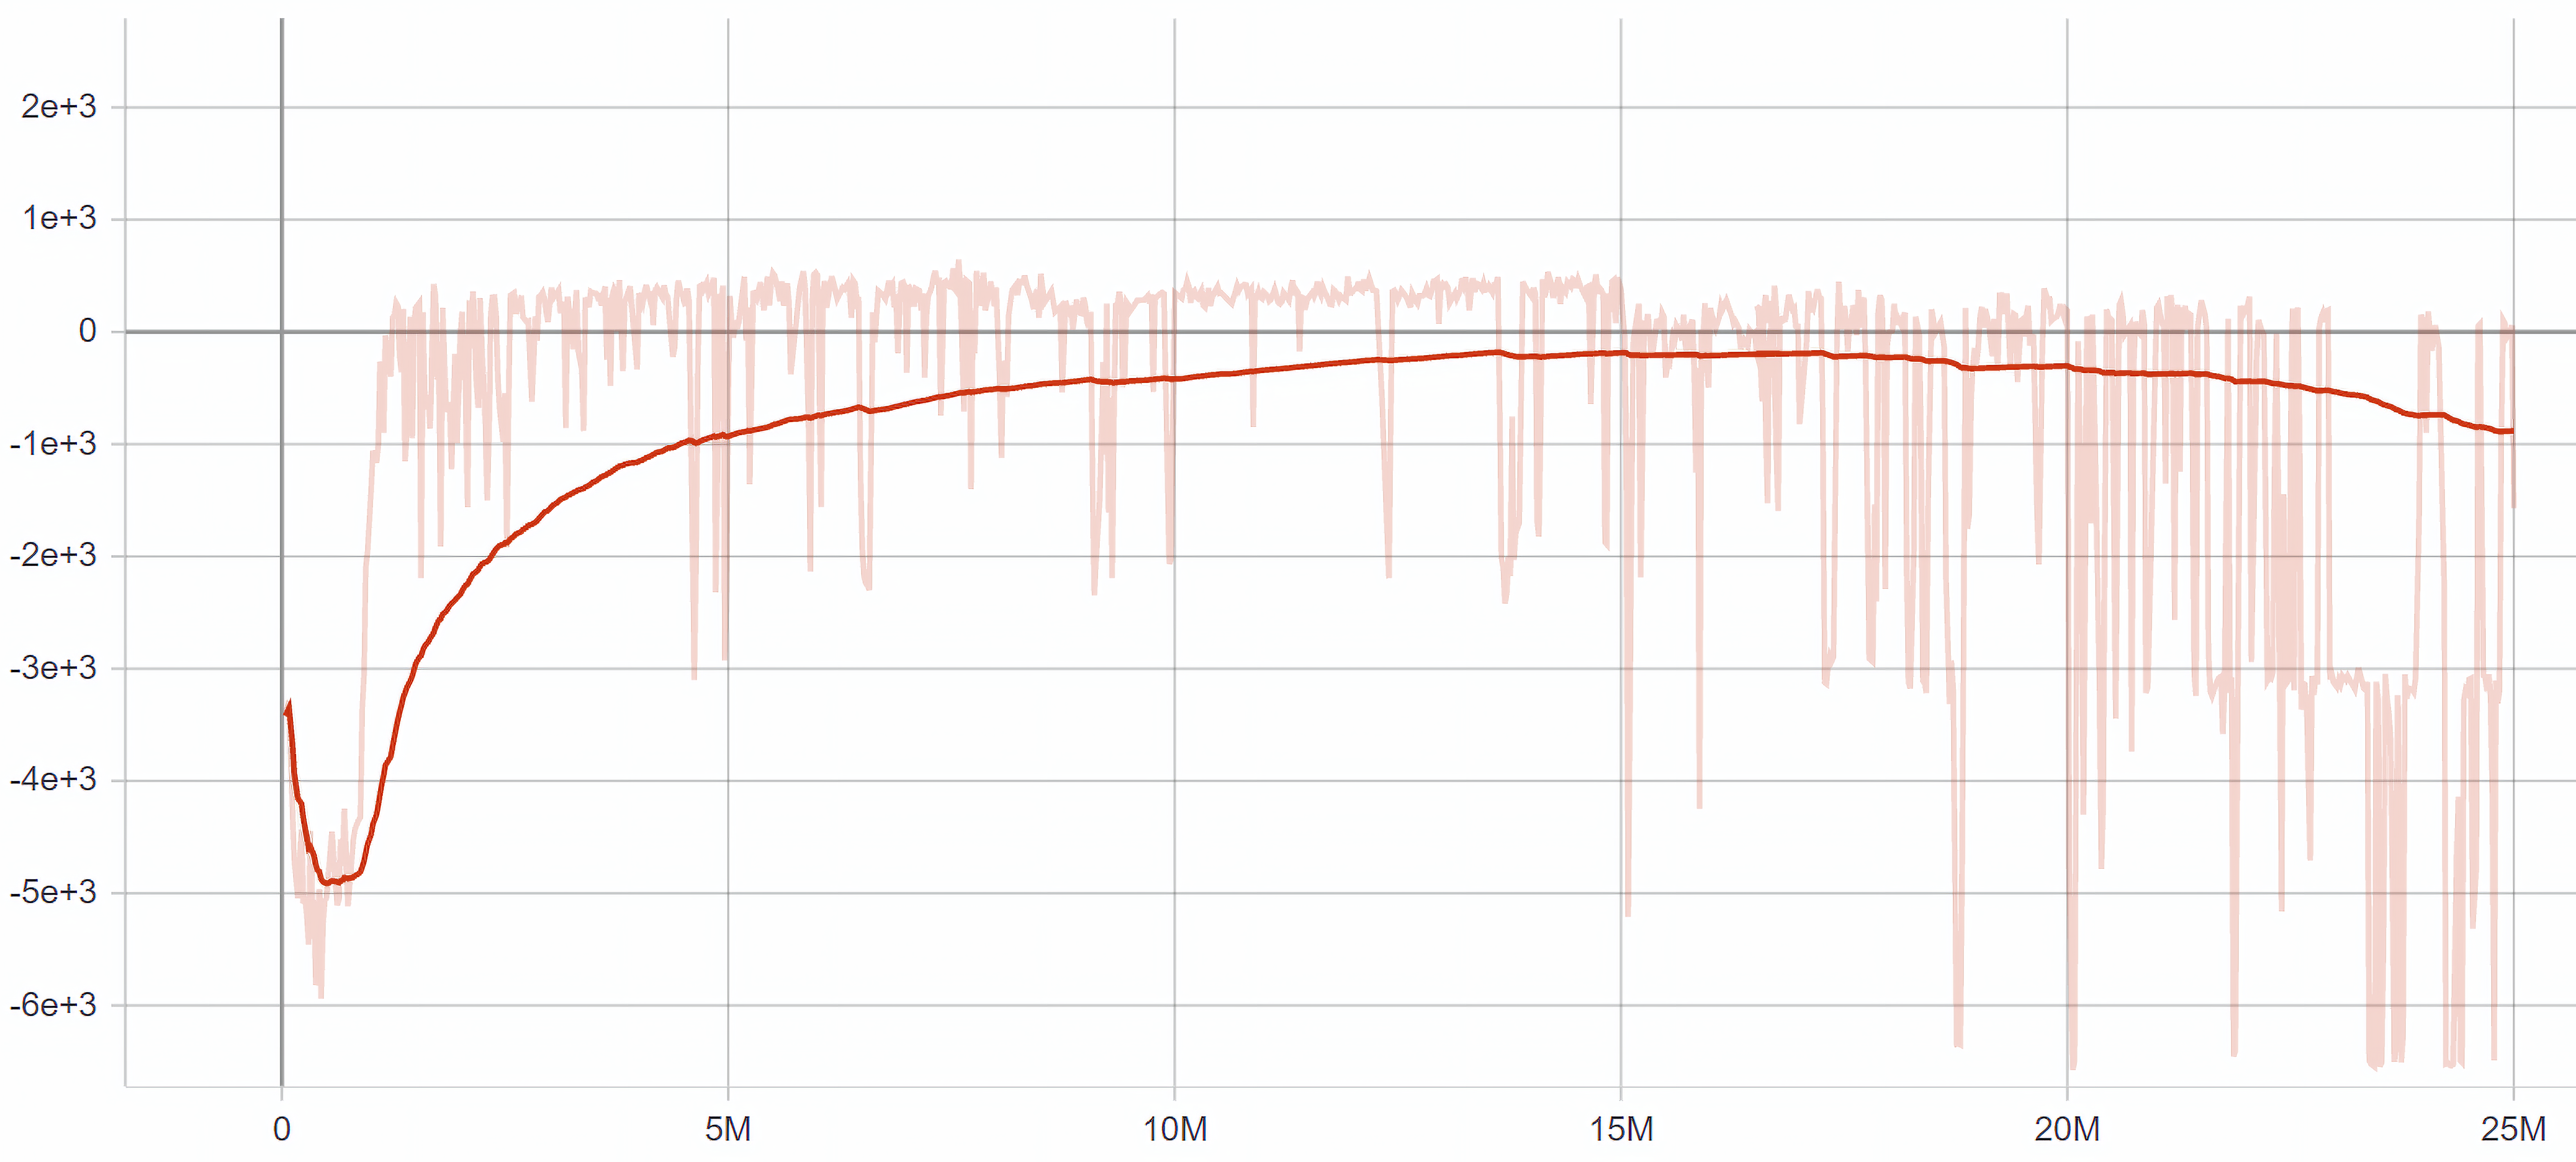
\includegraphics[scale=0.4]{Figures/Tensorboard4.PNG}
    \caption{Gap Error of 5 vehicles in the platoon}
\end{figure}
\end{comment}

Five tests with different scenarios are conducted to evaluate SDCP performance.
The first three test cases are conducted on a track of a straightforward road with no obstacles and the road turns to be able to focus more on the evaluation of the core principles of SDCP which are scalable platoon length, decentralization, and cooperation through the proposed sharing and caring communication topology. The fourth and fifth tests are conducted on the designed test track which is full of turns with tight radius of curvature and obstacles. %Table II shows the driving distance and the number of accidents occurred for each test case experiment.



\subsection{Test Scenario 1 $|$ Scalability}%(scalable platoon length)
\subsubsection{Pre-Testing Results}
The first test is to evaluate how the platoon can handle increasing its length from just three cars to five vehicles and then to eight connected cars, one leader, and seven followers.
Figures 11 and 12 show the gap error tracking between vehicles in the case of three vehicles and five vehicles, as a test case for scalability, respectively. After increasing the number of vehicles in the platoon to five vehicles, the gap errors between vehicles were not affected heavily and they focused on minimizing the gap error between them to minimal values as shown in the below tables(III, IV).

\begin{table}
\centering
\caption{Performance metrics for the three vehicles platoon} 
\resizebox{8.5cm}{!}{
\renewcommand{\arraystretch}{1.5}
\begin{tabular} {|c||c|c|c|c|} 
\hline
\textbf{Evaluation metrics} & \textbf{$RMSE_{Gap1}$} & \textbf{$RMSE_{Gap2}$} & \textbf{$Std_{Gap1}$} & \textbf{$Std_{Gap2}$}\\
\hline
Value (meters) & 1.45 & 0.84 & 1.01 & 0.46\\ 
\hline
\textbf{Evaluation metrics} & \textbf{$Max_{Gap1}$} & \textbf{$Max_{Gap2}$}& \textbf{$Stall_{Gap1}$} & \textbf{$Stall_{Gap2}$}\\
\hline
Value (meters) & 2.8 & 1.5 & 0 & 0.3\\ 
\hline
\end{tabular} }
\end{table}


\begin{table}
\centering
\caption{Performance metrics for the five vehicles platoon} 
\resizebox{8.5cm}{!}{
\renewcommand{\arraystretch}{1.5}
\begin{tabular} {|c||c|c|c|c|} 
 \hline
 \textbf{Evaluation metrics} & \textbf{$RMSE_{Gap1}$} & \textbf{$RMSE_{Gap2}$} & \textbf{$RMSE_{Gap3}$} & \textbf{$RMSE_{Gap4}$}\\
\hline
Value (meters) & 1.56 & 0.86 & 0.09 & 0.47\\ 
\hline
\textbf{Evaluation metrics} & \textbf{$Std_{Gap1}$} & \textbf{$Std_{Gap2}$} & \textbf{$Std_{Gap3}$} & \textbf{$Std_{Gap4}$}\\
\hline
Value (meters) & 1.01 & 0.47 & 0.08 & 0.13\\ 
\hline
\textbf{Evaluation metrics} & \textbf{$Max_{Gap1}$} & \textbf{$Max_{Gap2}$} & \textbf{$Max_{Gap3}$} & \textbf{$Max_{Gap4}$}\\
\hline
Value (meters) & 3 & 1.5 & -0.2 & -0.7\\ 
\hline
\textbf{Evaluation metrics} & \textbf{$Stall_{Gap1}$} & \textbf{$Stall_{Gap2}$} & \textbf{$Stall_{Gap3}$} & \textbf{$Stall_{Gap4}$}\\
\hline
Value (meters) & 0 & 0.2 & 0.1 & -0.5\\ 
\hline
\end{tabular} }
\end{table}


\begin{comment}
\begin{table}[H]
\centering
\caption{Performance metrics for the five vehicles platoon} 
\resizebox{8.5cm}{!}{
\renewcommand{\arraystretch}{2}
\begin{tabular} {|c||c|c|c|c|c|c|} 
 \hline
 \textbf{Evaluation metrics} & \textbf{$RMSE_{Gap1}$} & \textbf{$RMSE_{Gap2}$} & \textbf{$Std_{Gap1}$} & \textbf{$Std_{Gap2}$} & \textbf{$Stall_{Gap1}$} & \textbf{$Stall_{Gap2}$}\\
\hline
Value (meters) & 1.56 & 0.86 & 1.01 & 0.47 & 0 & 0.2\\ 
\hline
\textbf{Evaluation metrics} & \textbf{$RMSE_{Gap3}$} & \textbf{$RMSE_{Gap4}$} & \textbf{$Std_{Gap3}$} & \textbf{$Std_{Gap4}$} & \textbf{$Stall_{Gap3}$} & \textbf{$Stall_{Gap4}$}\\
\hline
Value (meters) & 0.09 & 0.47 & 0.08 & 0.13 & 0.1 & -0.5\\ 
\hline
\end{tabular} }
\end{table}
\end{comment}


\subsubsection{Scale up platoon length to eight vehicles}
From the gap and velocity curves in Figure 13, it is observed that follower vehicles wait till the leader starts driving and then start accelerating to minimize the gap error between the leader and the first two followers while gaps between other followers are almost within the desired gap of 10 meters as shown in Table V. Tracking vehicles' velocities also assure followers' actions of accelerating to keep up with the platoon formation and maintain string stability within the platoon, and to the best of our knowledge, no work has developed such algorithm that supports stable scalability to the number of vehicles in the platoon.

\begin{table}[H]
\centering
\caption{Performance metrics of the test scenario 1 (Eight vehicles platoon)} 
\resizebox{8.55cm}{!}{
\renewcommand{\arraystretch}{2.25}
\Large
\begin{tabular} {|c||c|c|c|c|c|c|c|} 
 \hline
 \textbf{Evaluation metrics} & \textbf{$RMSE_{Gap1}$} & \textbf{$RMSE_{Gap2}$} & \textbf{$RMSE_{Gap3}$} & \textbf{$RMSE_{Gap4}$} & \textbf{$RMSE_{Gap5}$} & \textbf{$RMSE_{Gap6}$} & \textbf{$RMSE_{Gap7}$}\\
\hline
Value (meters) & 1.66 & 1.07 & 0.37 & 0.65 & 0.45 & 0.38 & 0.34\\ 
\hline
\textbf{Evaluation metrics} & \textbf{$Std_{Gap1}$} & \textbf{$Std_{Gap2}$} & \textbf{$Std_{Gap3}$} & \textbf{$Std_{Gap4}$} & \textbf{$Std_{Gap5}$} & \textbf{$Std_{Gap6}$} & \textbf{$Std_{Gap7}$}\\
\hline
Value (meters) & 1.02 & 0.64 & 0.07 & 0.25 & 0.36 & 0.26 & 0.17\\ 
\hline
\textbf{Evaluation metrics} & \textbf{$Max_{Gap5}$} & \textbf{$Max_{Gap6}$} & \textbf{$Max_{Gap5}$} & \textbf{$Max_{Gap6}$} & \textbf{$Max_{Gap5}$} & \textbf{$Max_{Gap6}$} & \textbf{$Max_{Gap7}$}\\
\hline
Value (meters) & 3.1 & 2 & -0.4 & 0.7 & 0.1 & -0.4 & 0.1\\ 
\hline
\textbf{Evaluation metrics} & \textbf{$Stall_{Gap1}$} & \textbf{$Stall_{Gap2}$} & \textbf{$Stall_{Gap3}$} & \textbf{$Stall_{Gap4}$} & \textbf{$Stall_{Gap5}$} & \textbf{$Stall_{Gap6}$} & \textbf{$Stall_{Gap7}$}\\
\hline
Value (meters) & 0 & 0 & -0.4 & 0.7 & 0.1 & -0.4 & 0.1\\
\hline
\end{tabular} }
\end{table}


\begin{figure}
    \centering
    %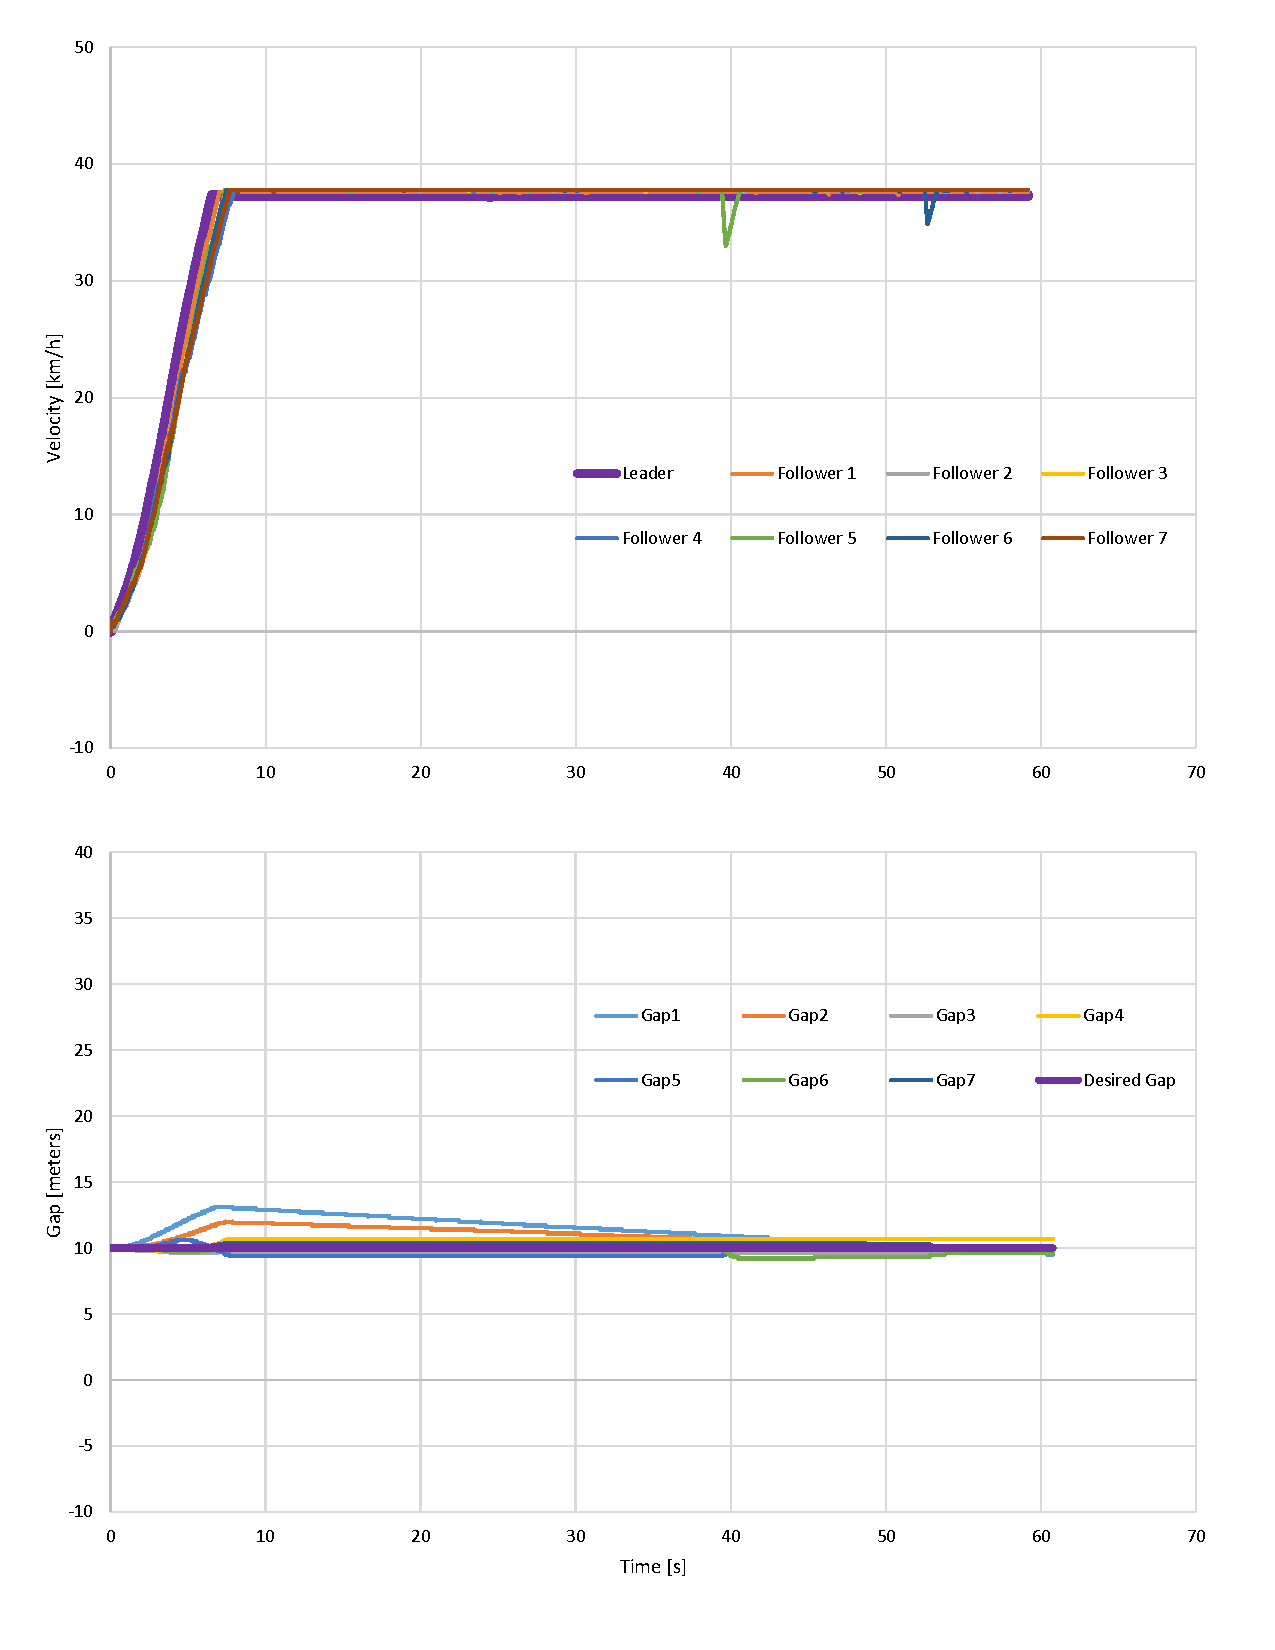
\includegraphics[width=1\linewidth]{Figures/EXP17_compressed.pdf}
    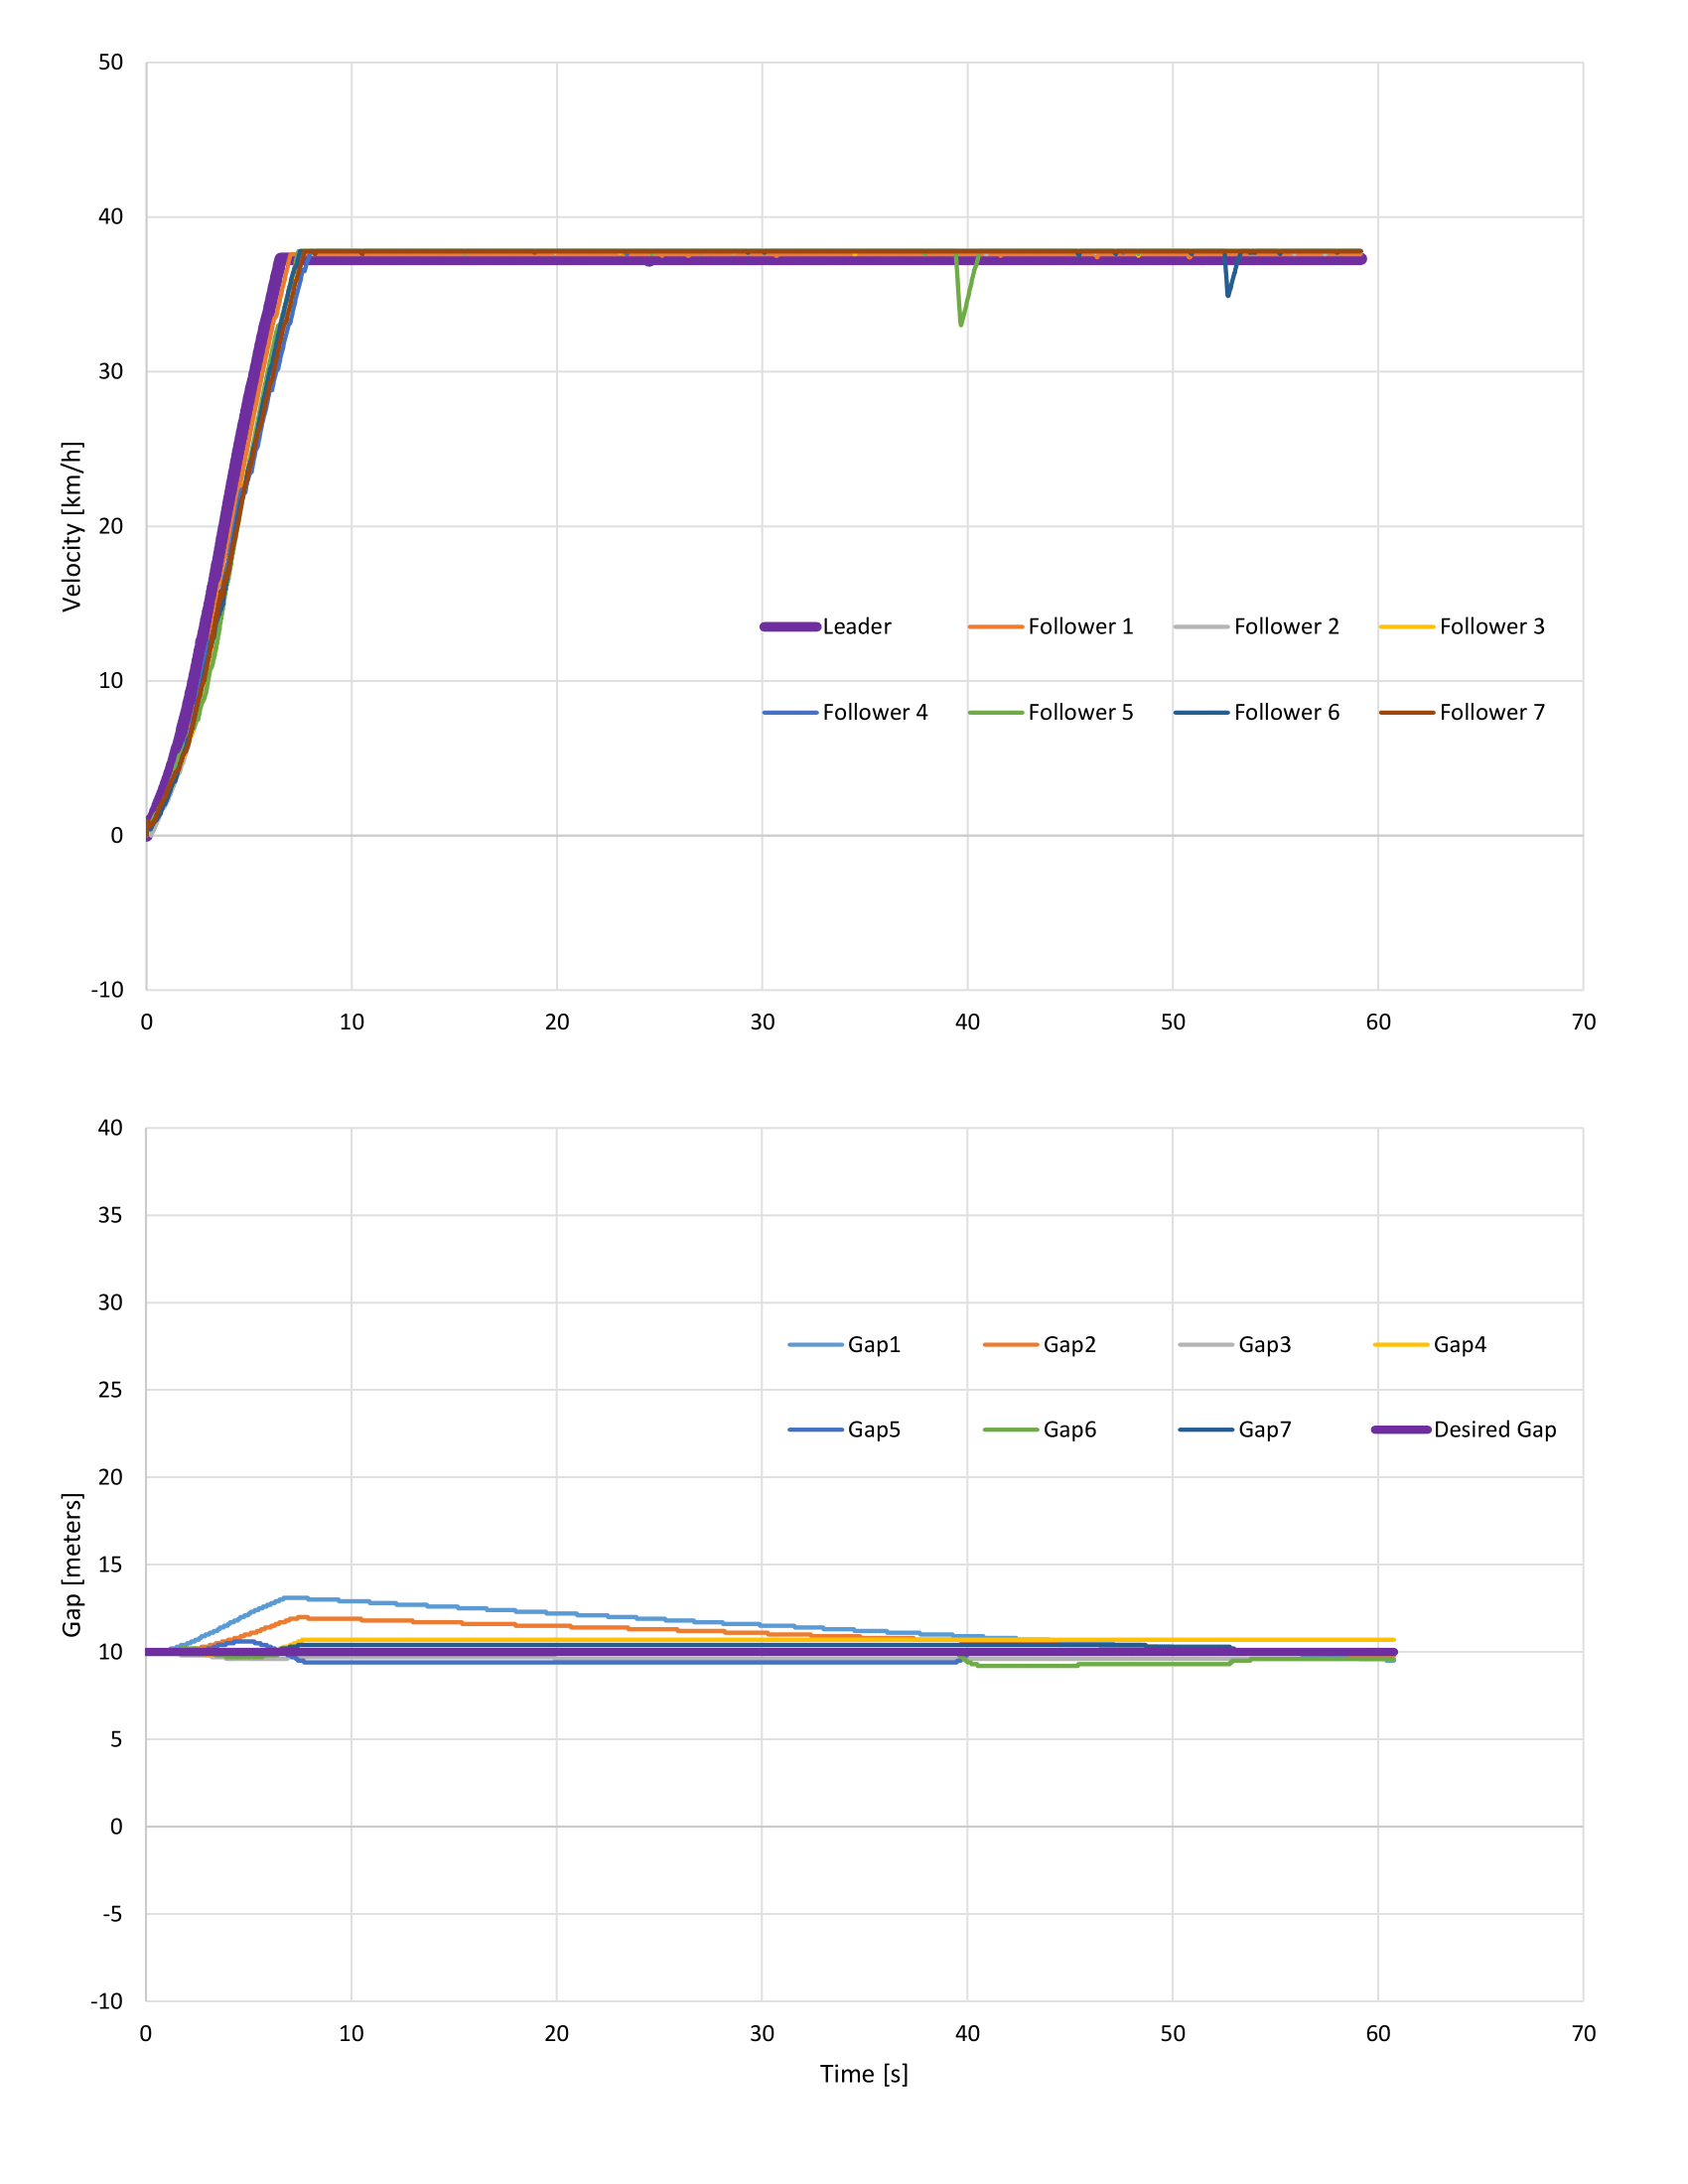
\includegraphics[width=1\linewidth]{Figures/EXP17-png.png}
    %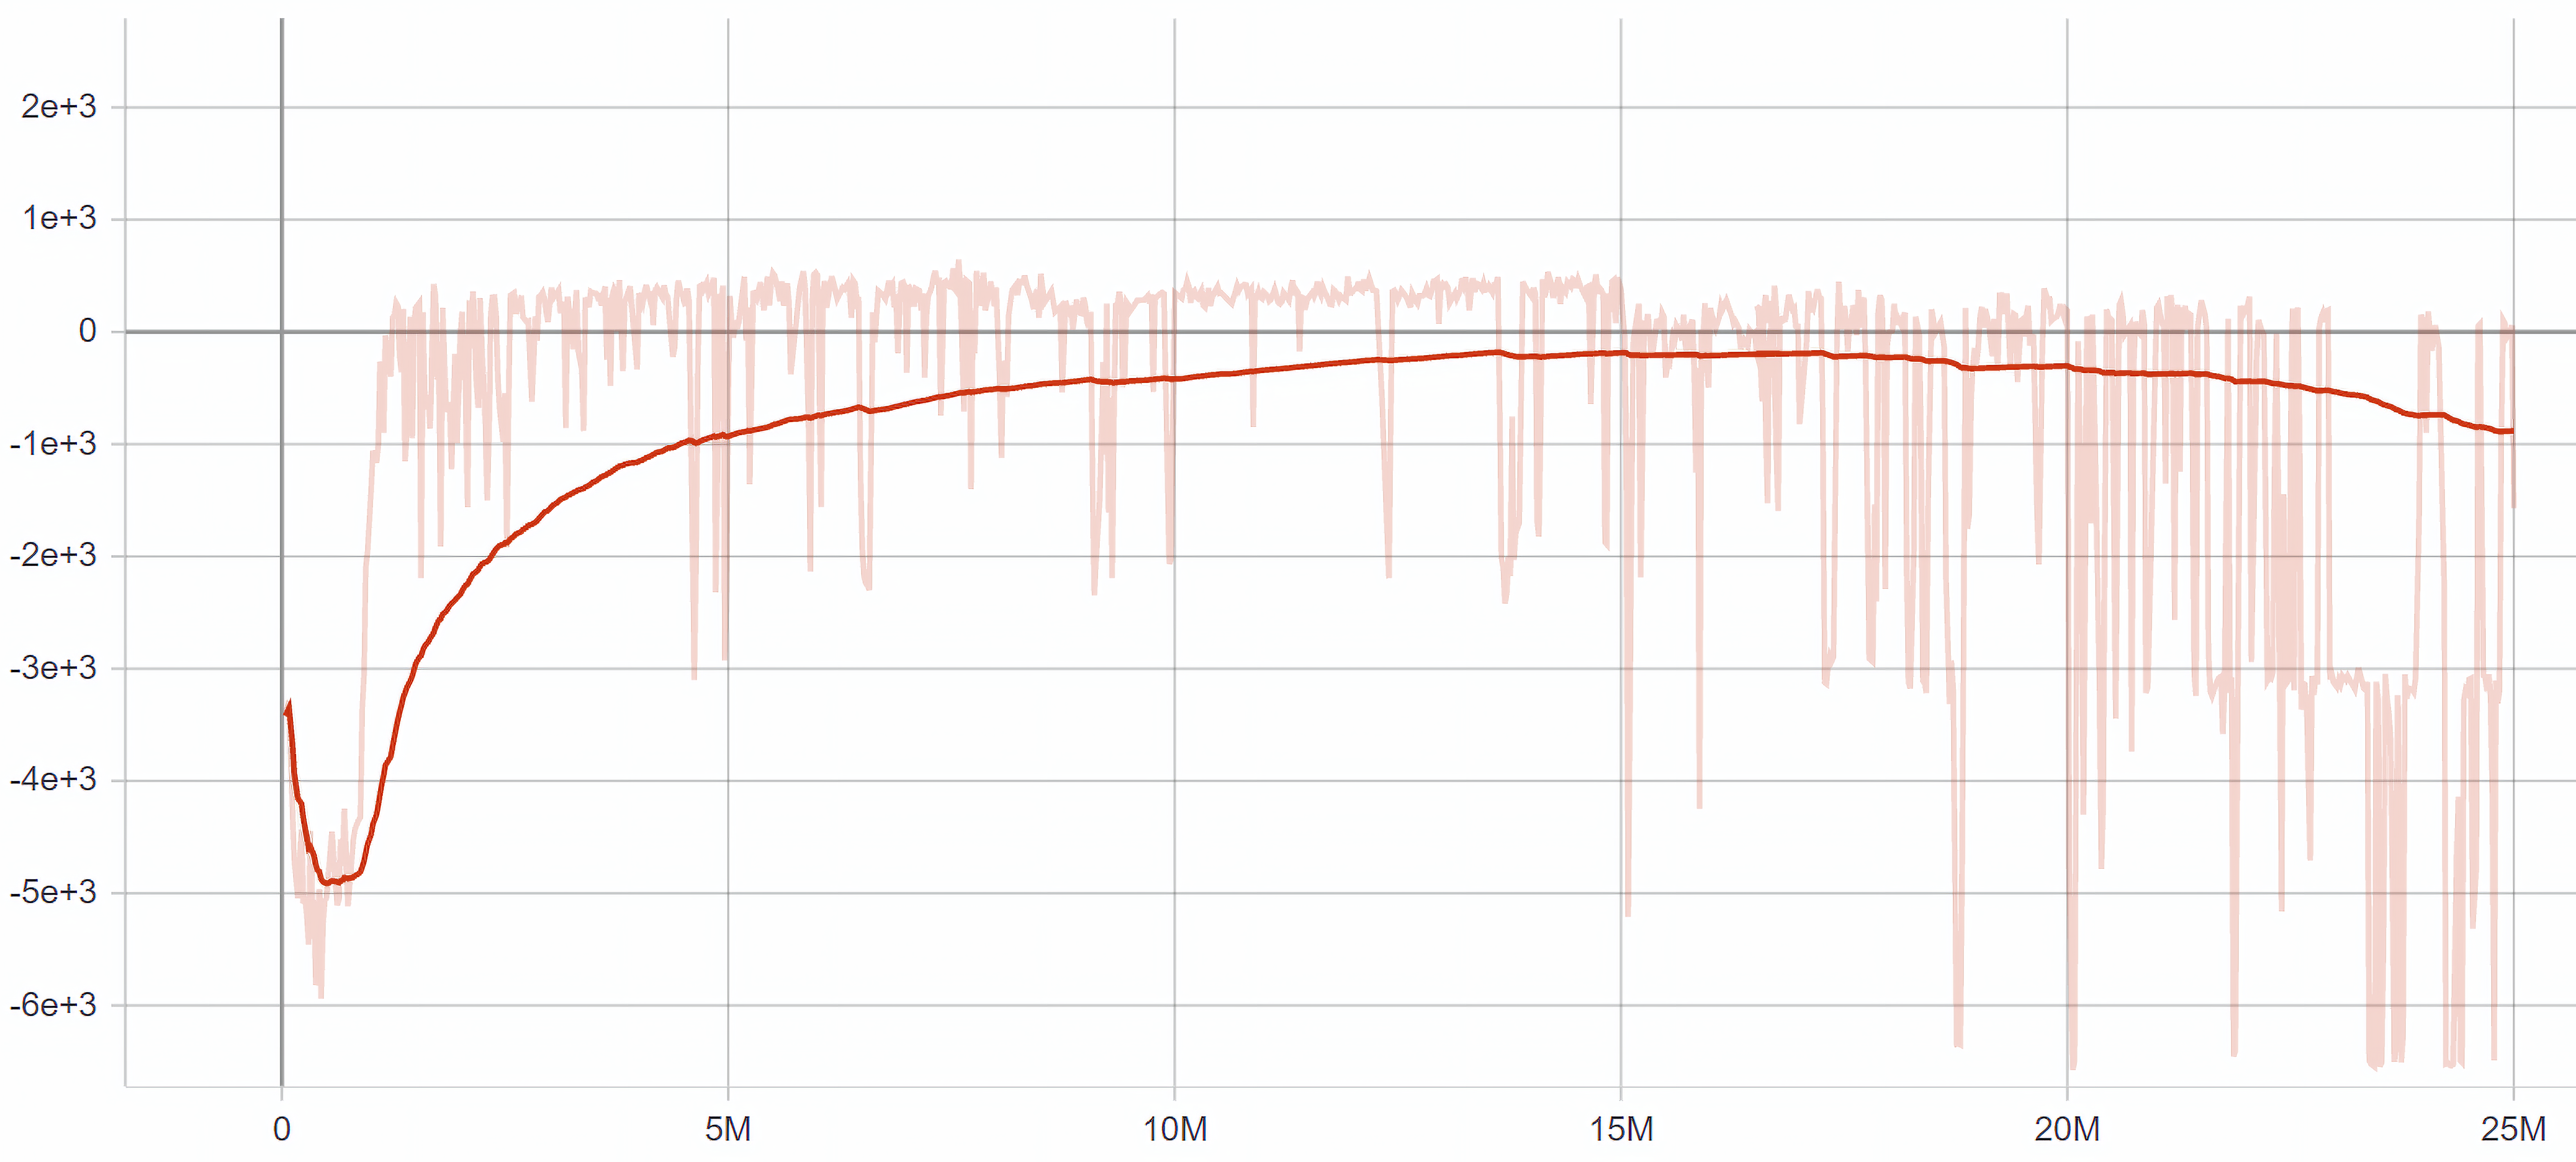
\includegraphics[scale=0.4]{Figures/Tensorboard4.PNG}
    \caption{Gap and Velocity Tracking of Test Case 1 (eight vehicles platoon)}
\end{figure}

\begin{comment}
\begin{figure}
\centering
\begin{subfigure}[b]{0.5\textwidth}
   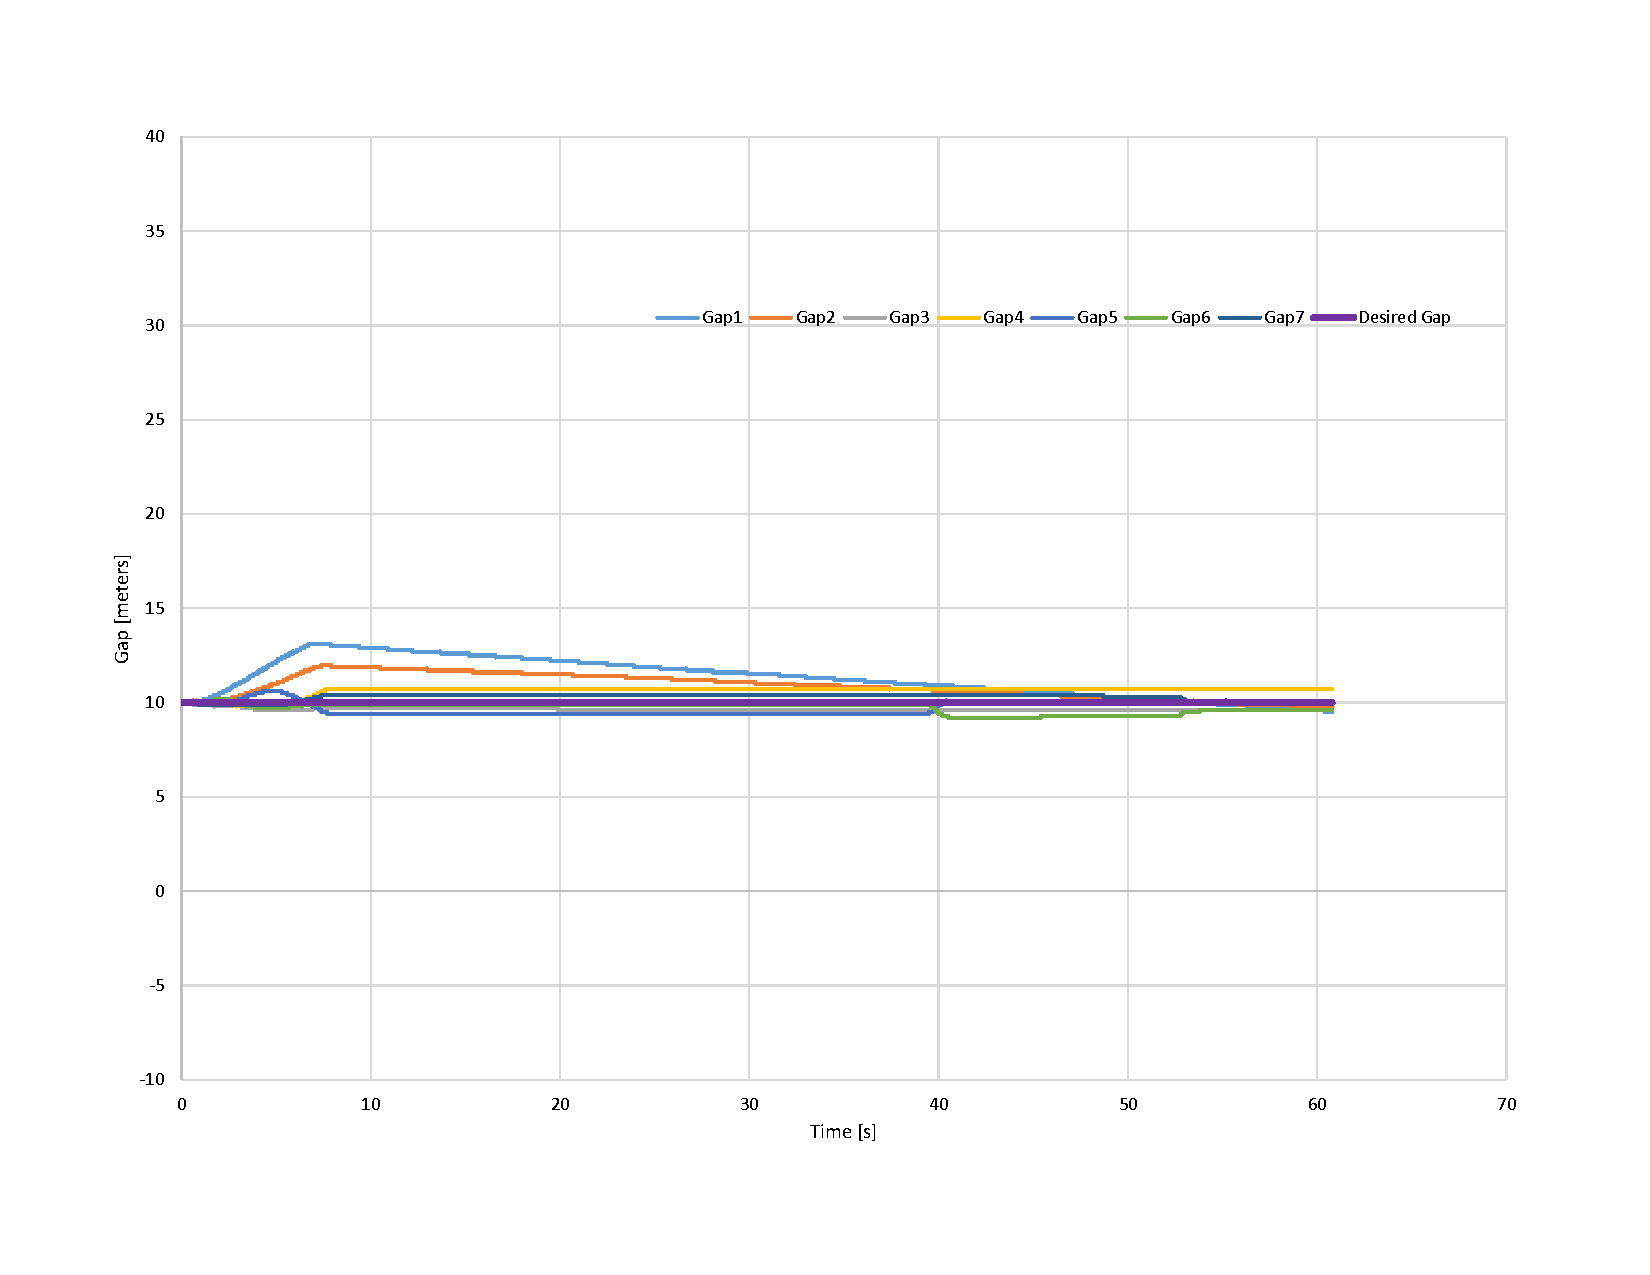
\includegraphics[width=1\linewidth]{Figures/Gap-EXP17.pdf}
   %\includegraphics[width=1\linewidth,height=40mm]{GapFigure(S)5.png}
   \label{fig:Ng1} 
\end{subfigure}

\begin{subfigure}[b]{0.5\textwidth}
   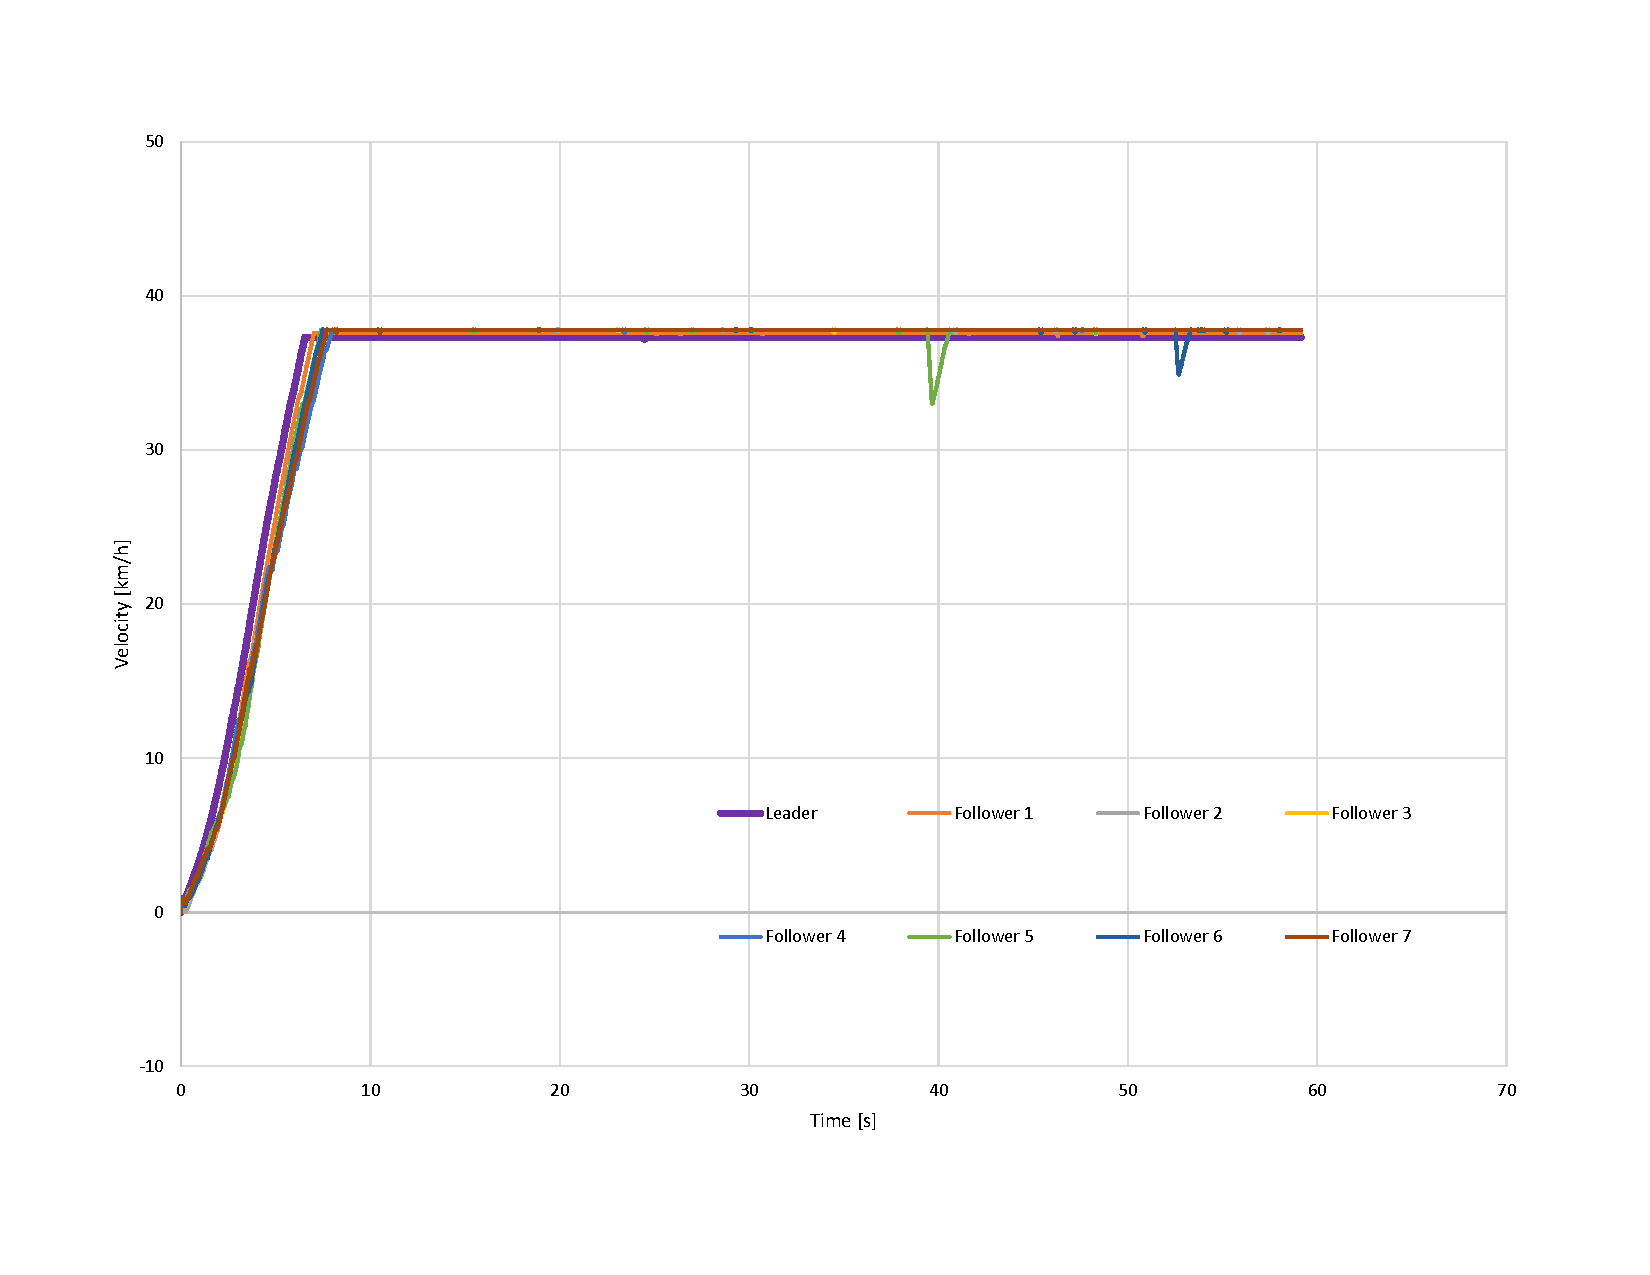
\includegraphics[width=1\linewidth]{Speeds-EXP17.pdf}
   %\includegraphics[width=1\linewidth,height=40mm]{VelocityFigure(S)5.png}
   \label{fig:Ng2}
\end{subfigure}

\caption[]{Gap and Velocity Tracking of Test Case 1}
\end{figure}


\begin{figure}
 \subfloat{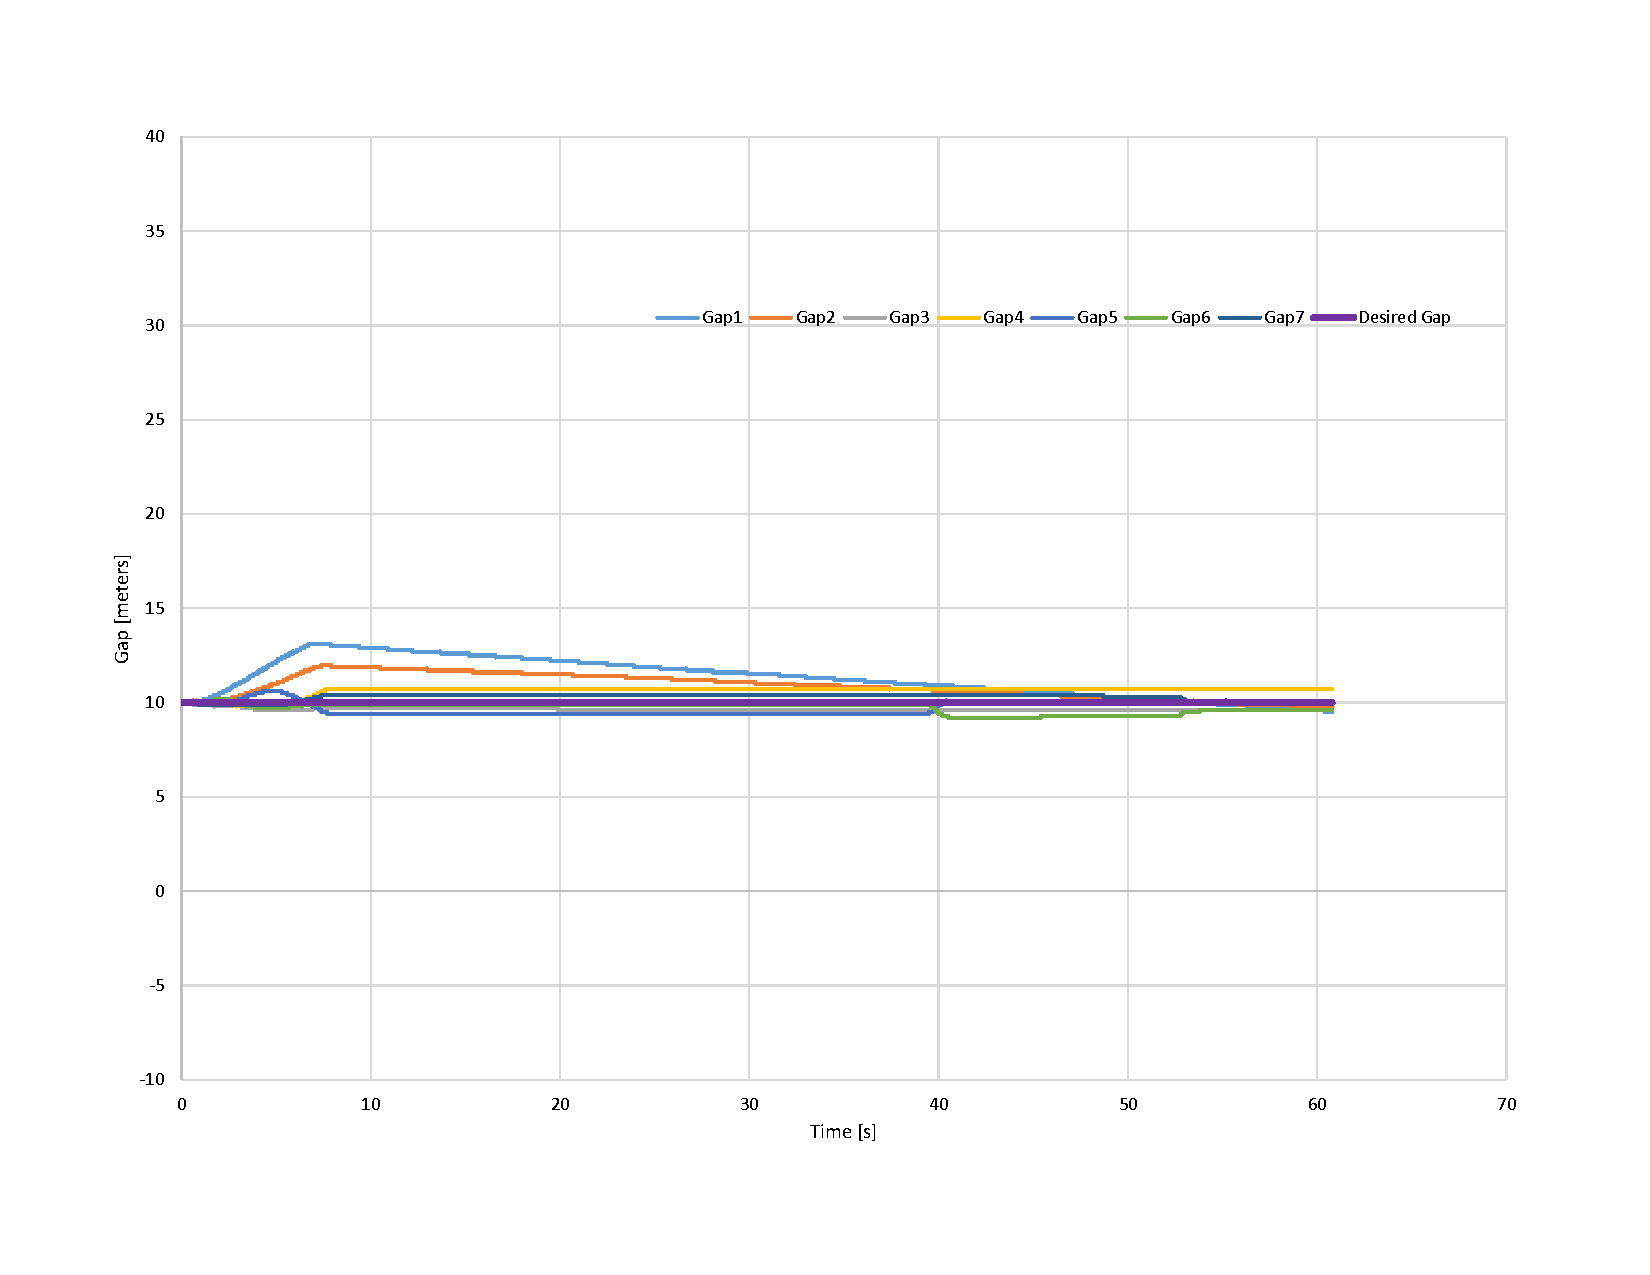
\includegraphics[width=0.5\textwidth]{Figures/Gap-EXP17.pdf}}\hfill
 \subfloat{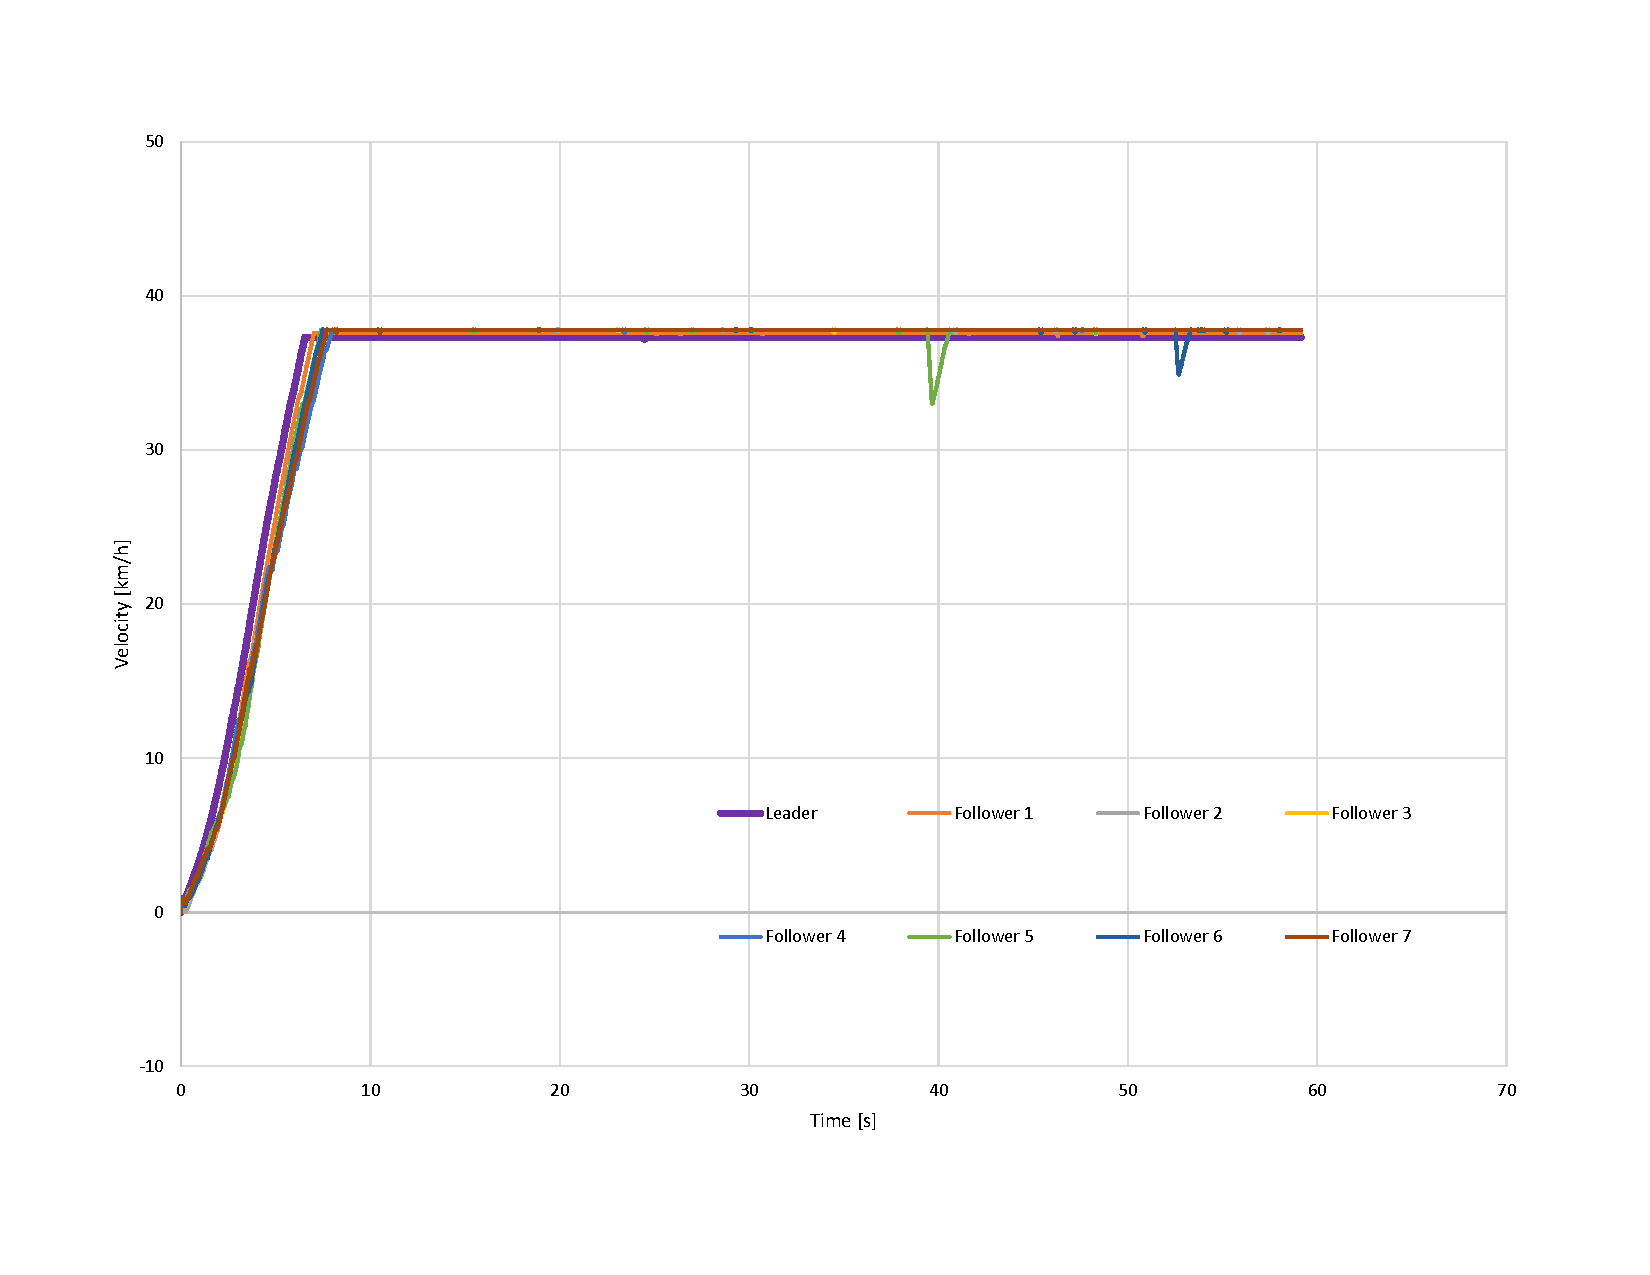
\includegraphics[width=0.5\textwidth]{Speeds-EXP17.pdf}}
 \caption{There are example figures}
\end{figure}
\end{comment}


\subsection{Test Scenario 2 $|$ Cooperation}%(Leader Aggressive Behavior, and safe driving)
The platoon's leader is subjected to aggressive behavior like a sudden change in its velocity to test the influence and coherence of the proposed communication topology on the cooperation between the vehicles in the platoon on mainly maintaining safe driving in dangerous scenarios. Figure 14 shows that vehicles behave in the first period as in test 1 accelerating to reach the desired gap between all vehicles, and then the leader's velocity suddenly decreases and keeps its speed for almost 10 seconds and then rapidly increases to its previous velocity. The platoon managed to adapt to the aggressive behavior from the leader with no crashes and decrease the gap errors between them, as shown in Table VI, but some gaps stalled with margins from the desired gap of 10 meters because of the adopted flexible spacing policy and all vehicles tend to drive at the max velocity to reach the finish line as soon as possible and collect more rewards.



\begin{table}
\centering
\caption{Performance metrics of the test scenario 2} 
\resizebox{8.55cm}{!}{
\renewcommand{\arraystretch}{2.25}
\Large
\begin{tabular} {|c||c|c|c|c|c|c|c|} 
 \hline
 \textbf{Evaluation metrics} & \textbf{$RMSE_{Gap1}$} & \textbf{$RMSE_{Gap2}$} & \textbf{$RMSE_{Gap3}$} & \textbf{$RMSE_{Gap4}$} & \textbf{$RMSE_{Gap5}$} & \textbf{$RMSE_{Gap6}$} & \textbf{$RMSE_{Gap7}$}\\
\hline
Value (meters) & 1.89 & 2.27 & 2.16 & 1.73 & 0.91 & 0.49 & 0.13\\ 
\hline
\textbf{Evaluation metrics} & \textbf{$Std_{Gap1}$} & \textbf{$Std_{Gap2}$} & \textbf{$Std_{Gap3}$} & \textbf{$Std_{Gap4}$} & \textbf{$Std_{Gap5}$} & \textbf{$Std_{Gap6}$} & \textbf{$Std_{Gap7}$}\\
\hline
Value (meters) & 1.72 & 2.17 & 1.60 & 1.67 & 0.60 & 0.30 & 0.12\\ 
\hline
\textbf{Evaluation metrics} & \textbf{$Max_{Gap5}$} & \textbf{$Max_{Gap6}$} & \textbf{$Max_{Gap5}$} & \textbf{$Max_{Gap6}$} & \textbf{$Max_{Gap5}$} & \textbf{$Max_{Gap6}$} & \textbf{$Max_{Gap7}$}\\
\hline
Value (meters) & 3.2 & -5.6 & -6 & -4.7 & -2.7 & -0.9 & -0.3\\ 
\hline
\textbf{Evaluation metrics} & \textbf{$Stall_{Gap1}$} & \textbf{$Stall_{Gap2}$} & \textbf{$Stall_{Gap3}$} & \textbf{$Stall_{Gap4}$} & \textbf{$Stall_{Gap5}$} & \textbf{$Stall_{Gap6}$} & \textbf{$Stall_{Gap7}$}\\
\hline
Value (meters) & -0.8 & -3.4 & -1.9 & -3.9 & -2.7 & -0.6 & -0.3\\
\hline
\end{tabular} }
\end{table}


\begin{figure}
    \centering
    %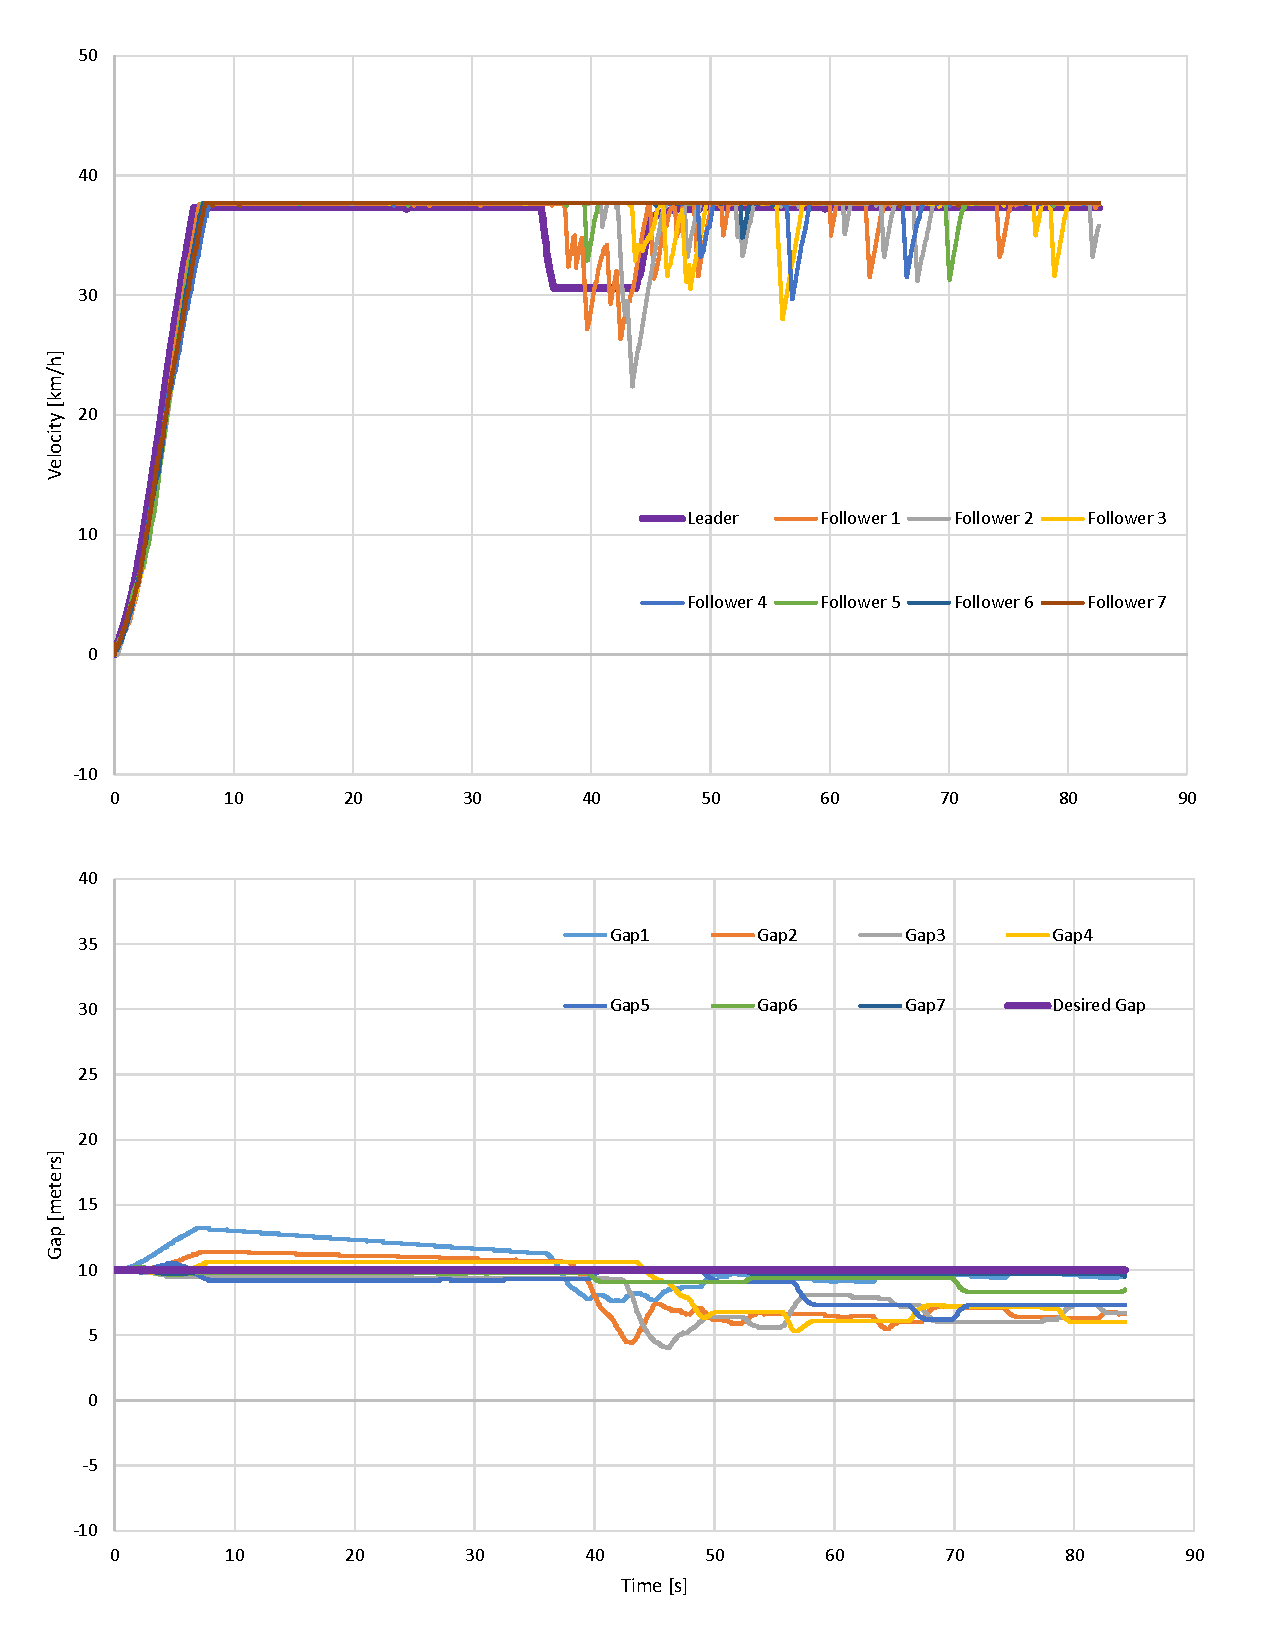
\includegraphics[width=1\linewidth]{Figures/Exp21_compressed.pdf}
    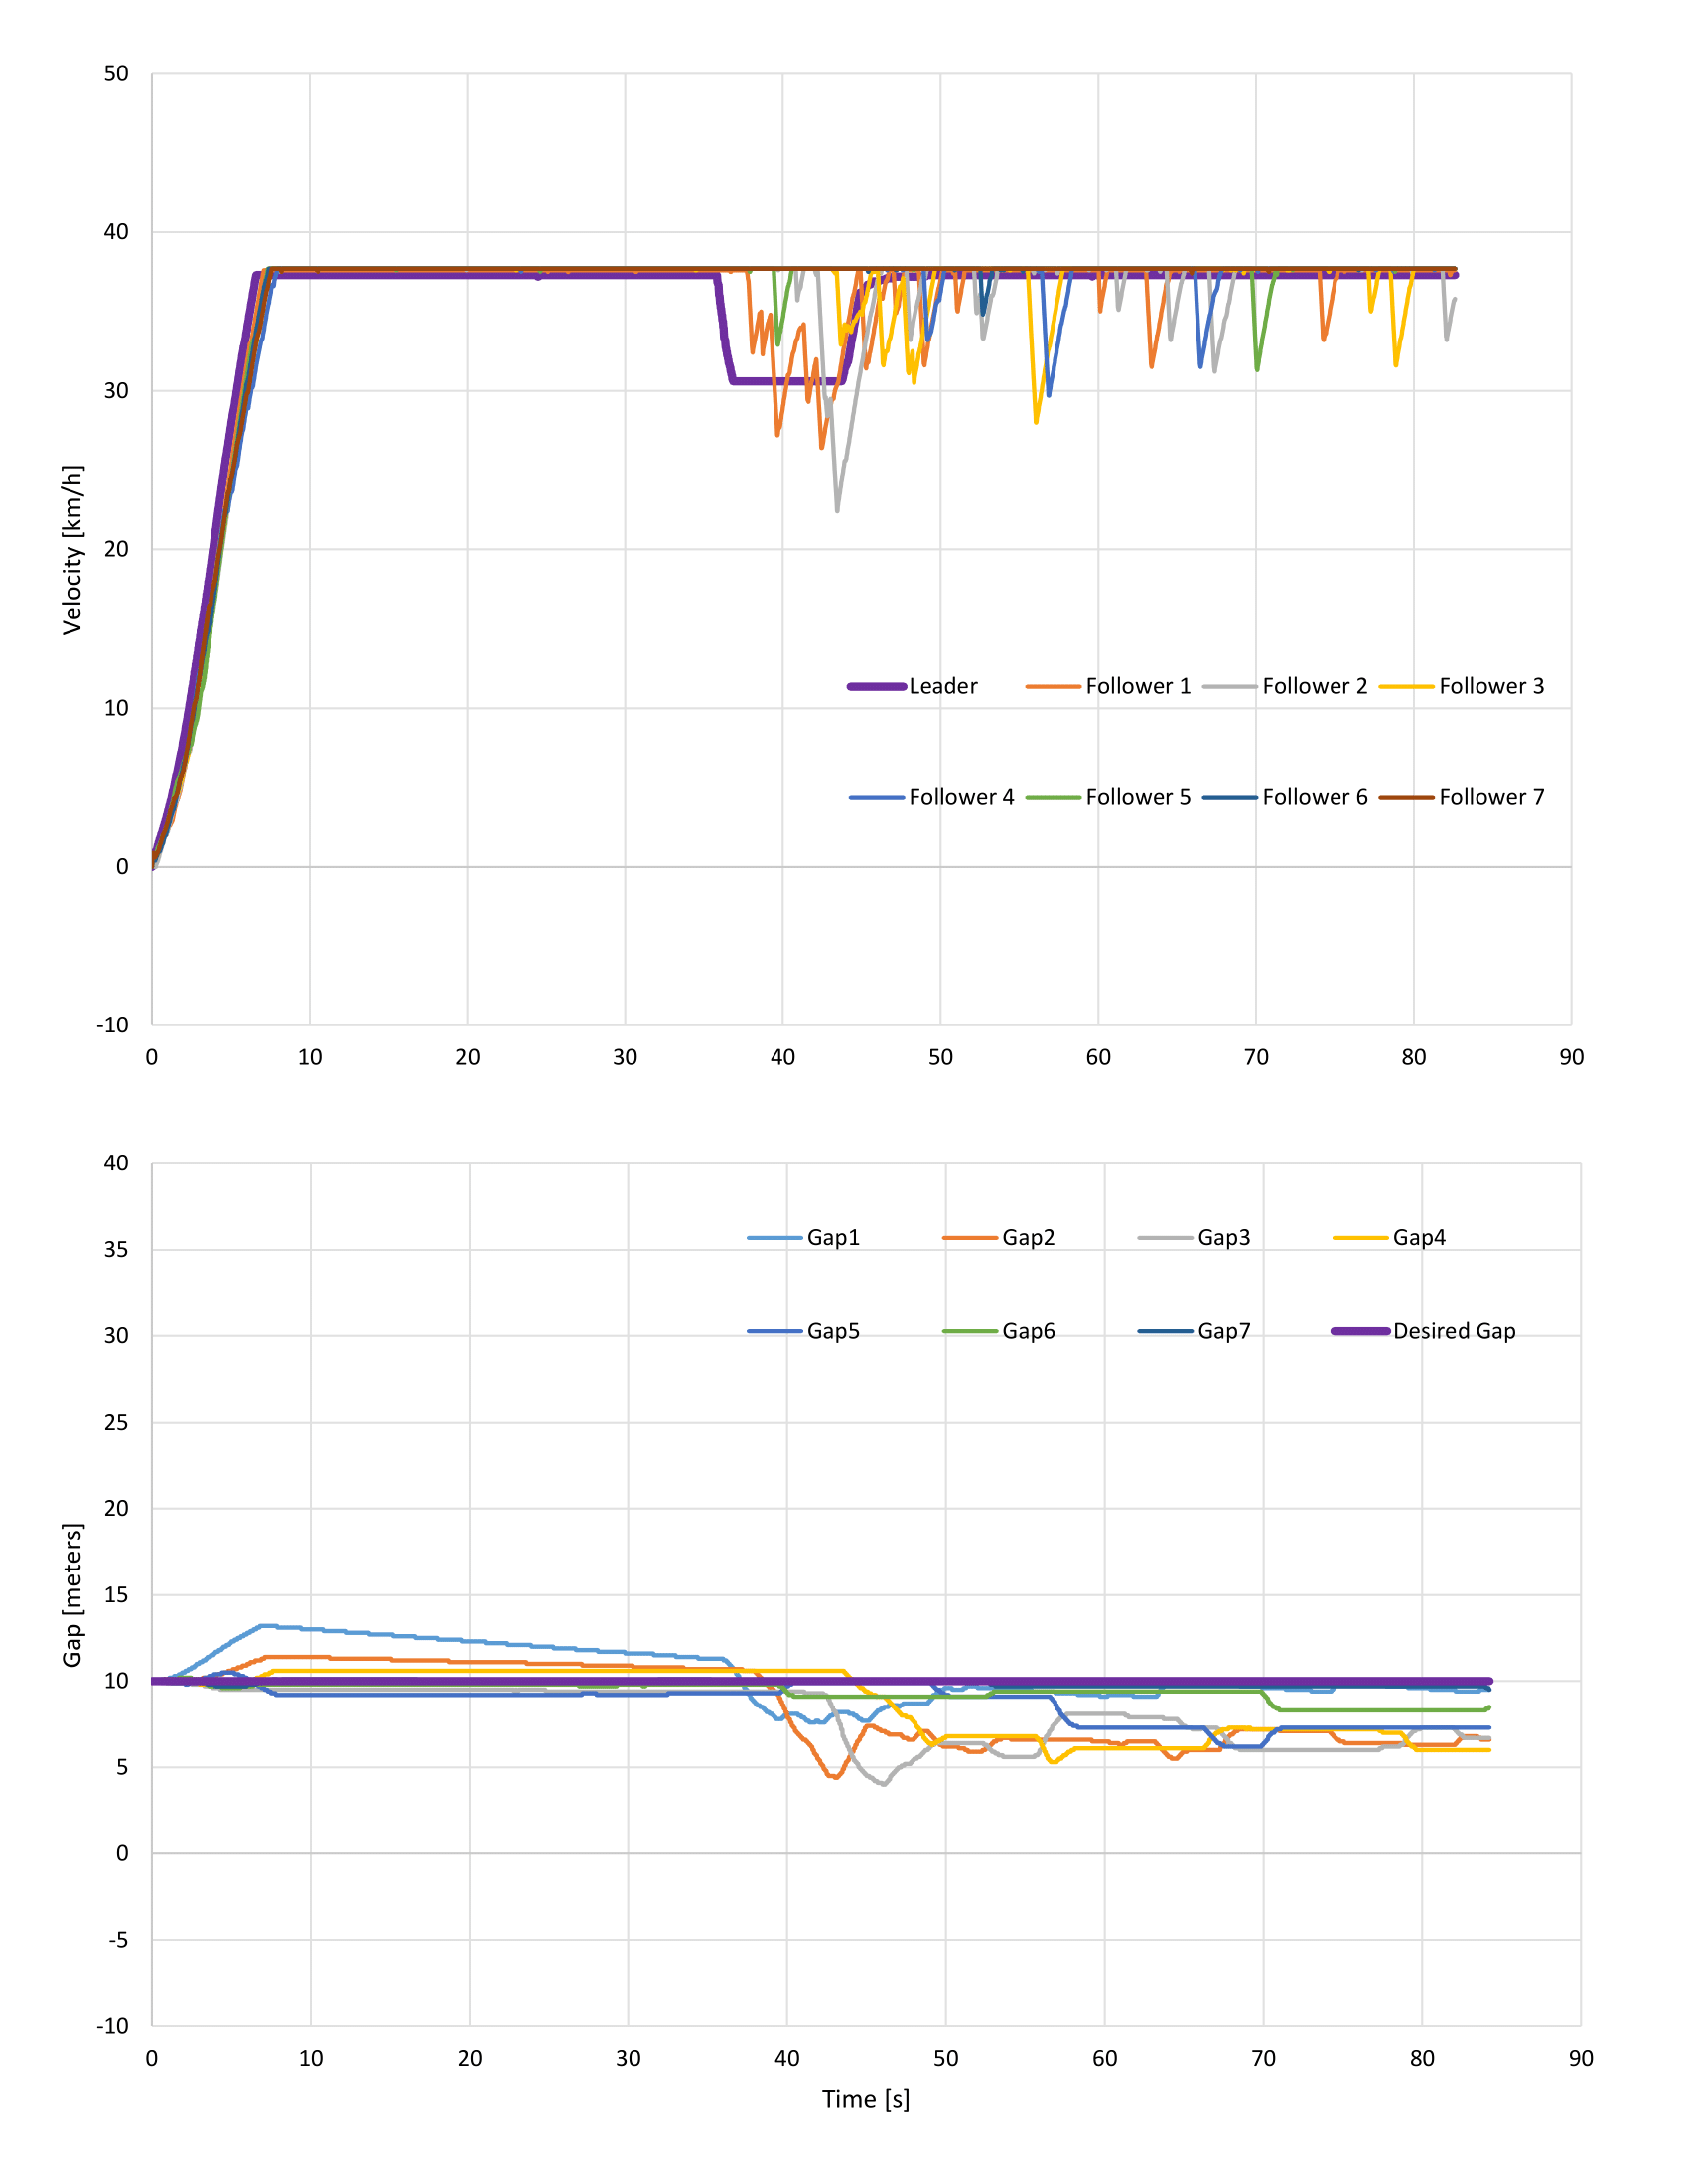
\includegraphics[width=1\linewidth]{Figures/Exp21-png.png}
    %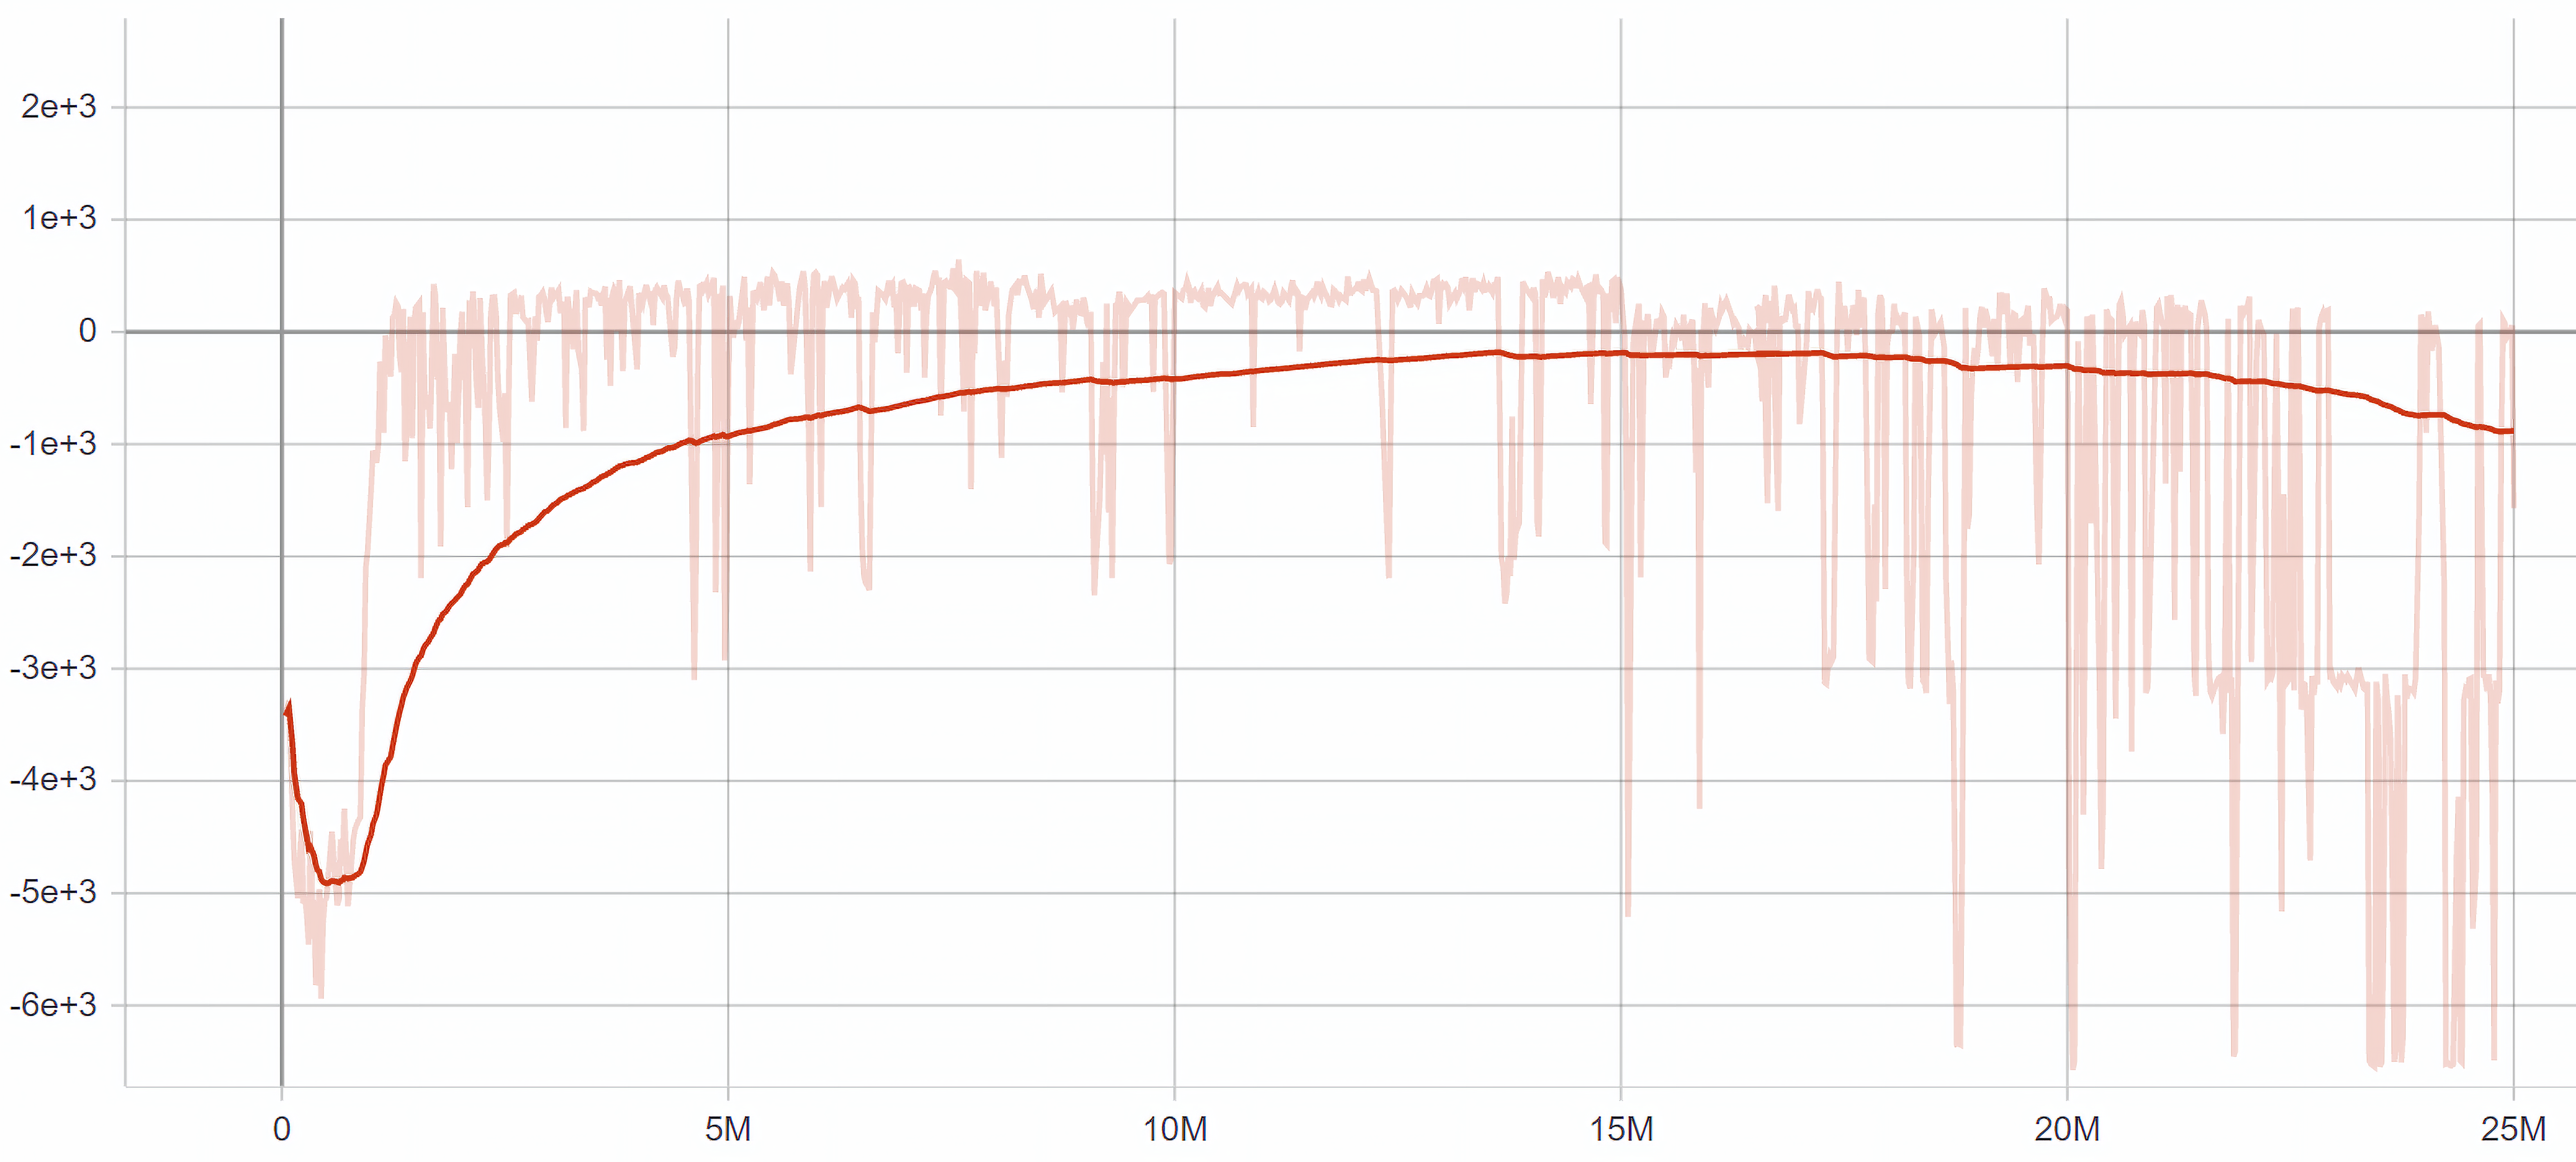
\includegraphics[scale=0.4]{Figures/Tensorboard4.PNG}
    \caption{Gap and Velocity Tracking of Test Case 2}
\end{figure}

\begin{comment}
\begin{figure}
\centering
\begin{subfigure}[b]{0.4\textwidth}
   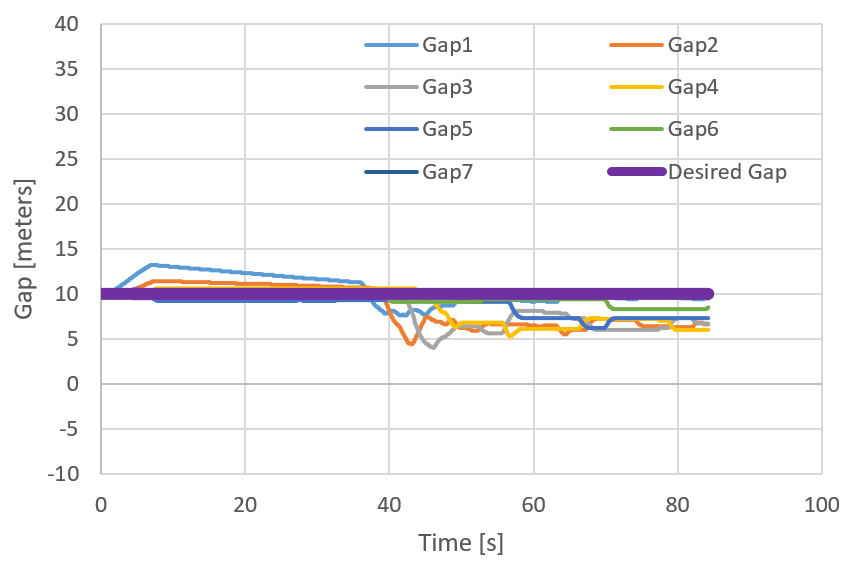
\includegraphics[width=1\linewidth]{Figures/EXP21_Gap.PNG}
   \label{fig:Ng1} 
\end{subfigure}

\begin{subfigure}[b]{0.4\textwidth}
   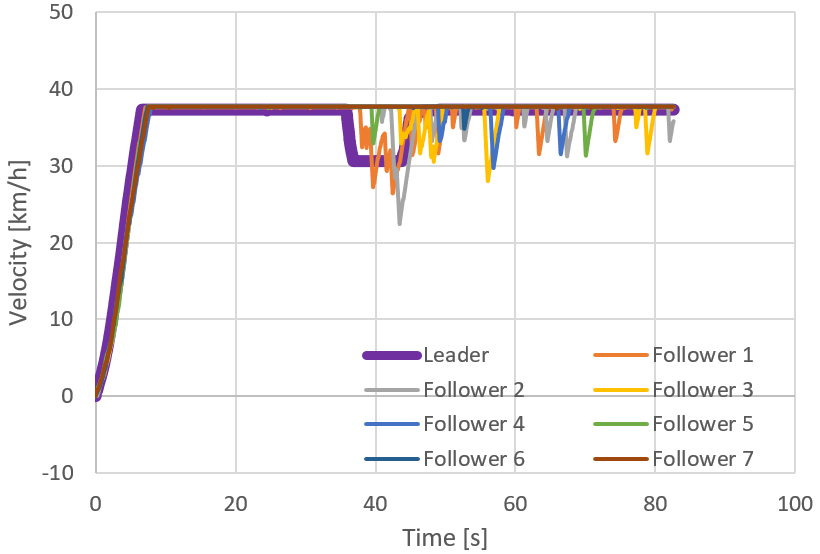
\includegraphics[width=1\linewidth]{Figures/EXP21_Vel.PNG}
   \label{fig:Ng2}
\end{subfigure}

\caption[]{Gap and Velocity Tracking of Test Case 2}
\end{figure}
\end{comment}


%"Exp15Final-png" "Exp20-png"
\subsection{Test Scenario 3 $|$ Decentralization}% (Leaderless Platoon Testing)
In this test, followers will be ordered to drive without the leader's vehicle and their performance is measured to be a clear validation of the decentralized behavior of the vehicles in the platoon. followers significantly are able to drive without the leader and continue depending on each other while sharing their perception data between them through V2V, and almost all of them maintained the desired gap with minimal errors, as shown in Table VII, and the same velocity between them as shown in figure 15. This is proof of one of the advantages of having a decentralized system for such cases the vehicles can handle emergency cases when the leader of the platoon, where followers are used to driving following it, is not able to drive and they should adapt to this new and unexpected circumstances.



\begin{table}
\centering
\caption{Performance metrics of the test scenario 3} 
\resizebox{8.55cm}{!}{
\renewcommand{\arraystretch}{2.25}
\Large
\begin{tabular} {|c||c|c|c|c|c|c|c|} 
 \hline
 \textbf{Evaluation metrics} & \textbf{$RMSE_{Gap1}$} & \textbf{$RMSE_{Gap2}$} & \textbf{$RMSE_{Gap3}$} & \textbf{$RMSE_{Gap4}$} & \textbf{$RMSE_{Gap5}$} & \textbf{$RMSE_{Gap6}$} & \textbf{$RMSE_{Gap7}$}\\
\hline
Value (meters) & 347.22 & 0.32 & 1.11 & 0.55 & 0.49 & 0.84 & 0.64\\ 
\hline
\textbf{Evaluation metrics} & \textbf{$Std_{Gap1}$} & \textbf{$Std_{Gap2}$} & \textbf{$Std_{Gap3}$} & \textbf{$Std_{Gap4}$} & \textbf{$Std_{Gap5}$} & \textbf{$Std_{Gap6}$} & \textbf{$Std_{Gap7}$}\\
\hline
Value (meters) & 141.26 & 0.30 & 0.37 & 0.20 & 0.18 & 0.28 & 0.15\\ 
\hline
\textbf{Evaluation metrics} & \textbf{$Max_{Gap5}$} & \textbf{$Max_{Gap6}$} & \textbf{$Max_{Gap5}$} & \textbf{$Max_{Gap6}$} & \textbf{$Max_{Gap5}$} & \textbf{$Max_{Gap6}$} & \textbf{$Max_{Gap7}$}\\
\hline
Value (meters) & 441.8 & 1.6 & -1.5 & -1 & 0.6 & -1 & -0.8\\ 
\hline
\textbf{Evaluation metrics} & \textbf{$Stall_{Gap1}$} & \textbf{$Stall_{Gap2}$} & \textbf{$Stall_{Gap3}$} & \textbf{$Stall_{Gap4}$} & \textbf{$Stall_{Gap5}$} & \textbf{$Stall_{Gap6}$} & \textbf{$Stall_{Gap7}$}\\
\hline
Value (meters) & 441.8 & 0.2 & -0.6 & -0.9 & 0.5 & -0.7 & -0.8\\
\hline
\end{tabular} }
\end{table}



\begin{figure}
    \centering
    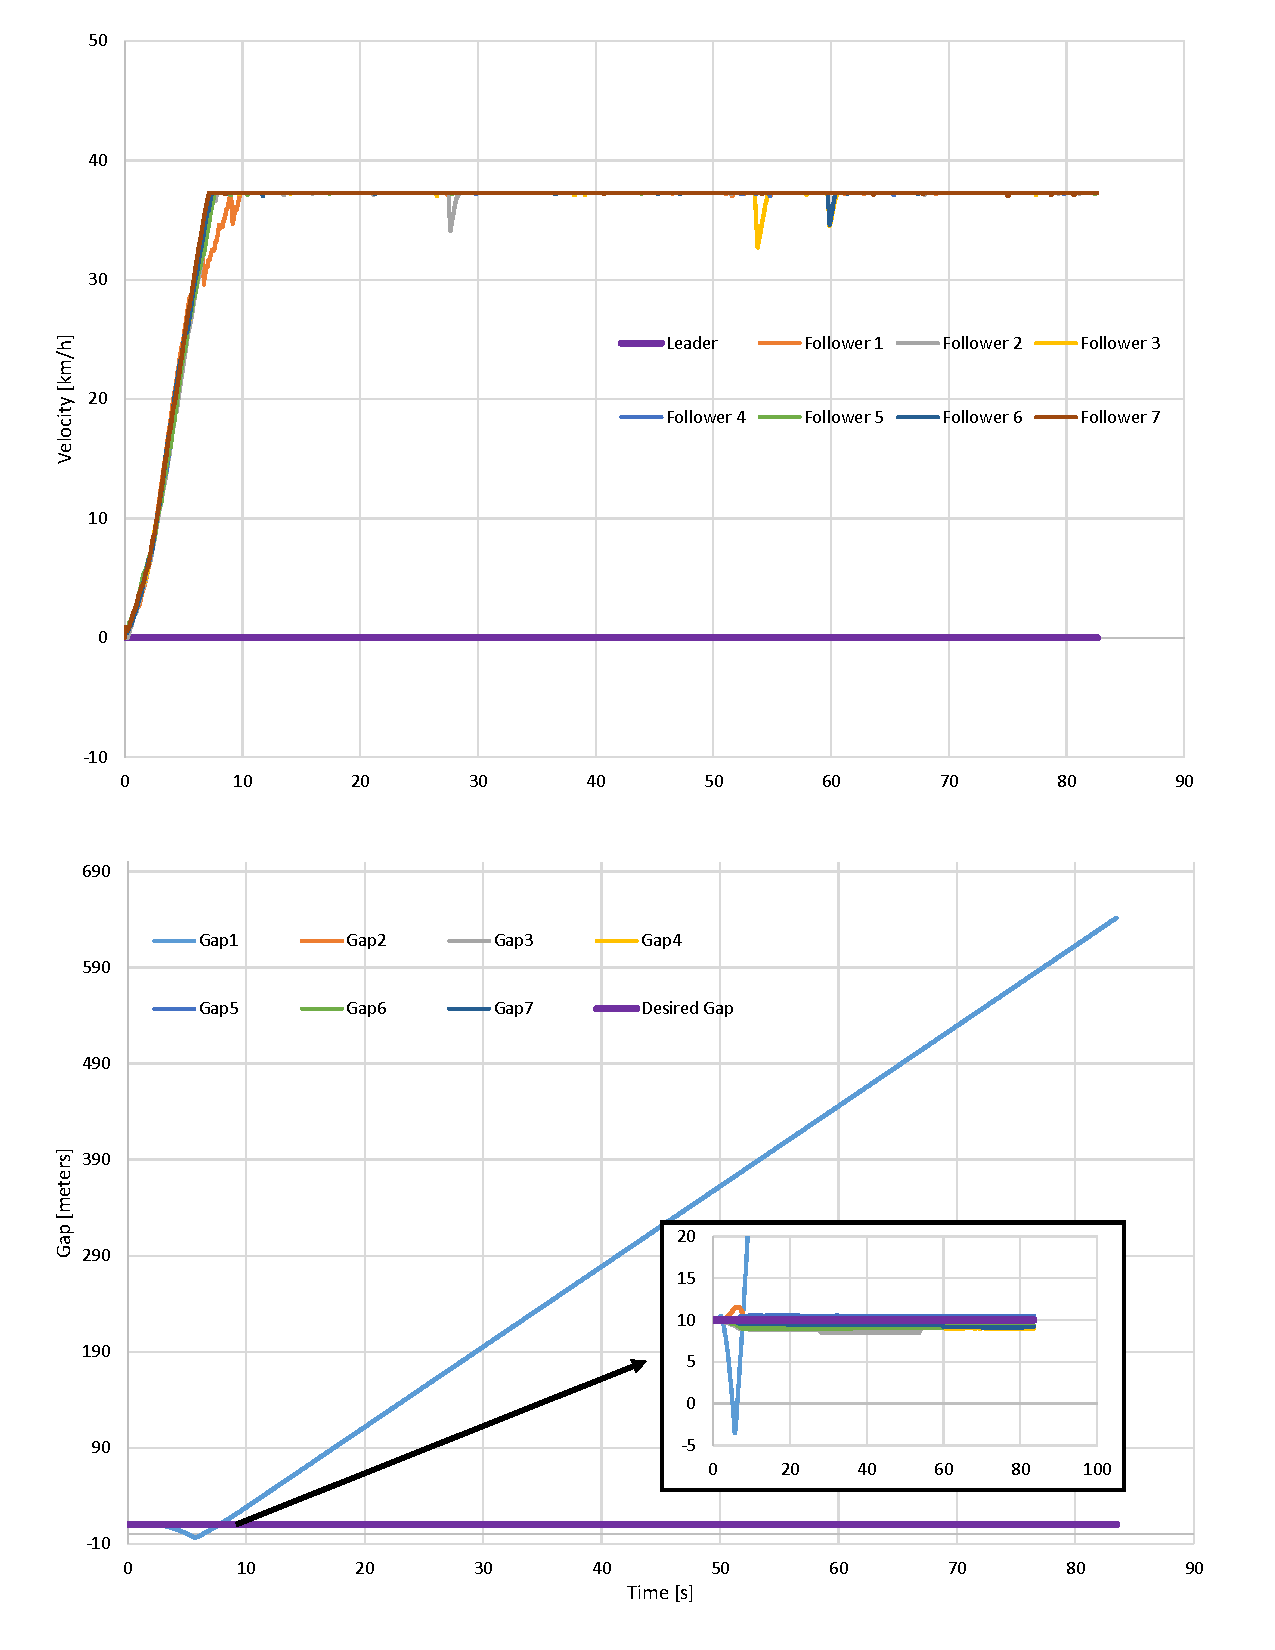
\includegraphics[width=1\linewidth]{Figures/Exp20_compressed.pdf}
    %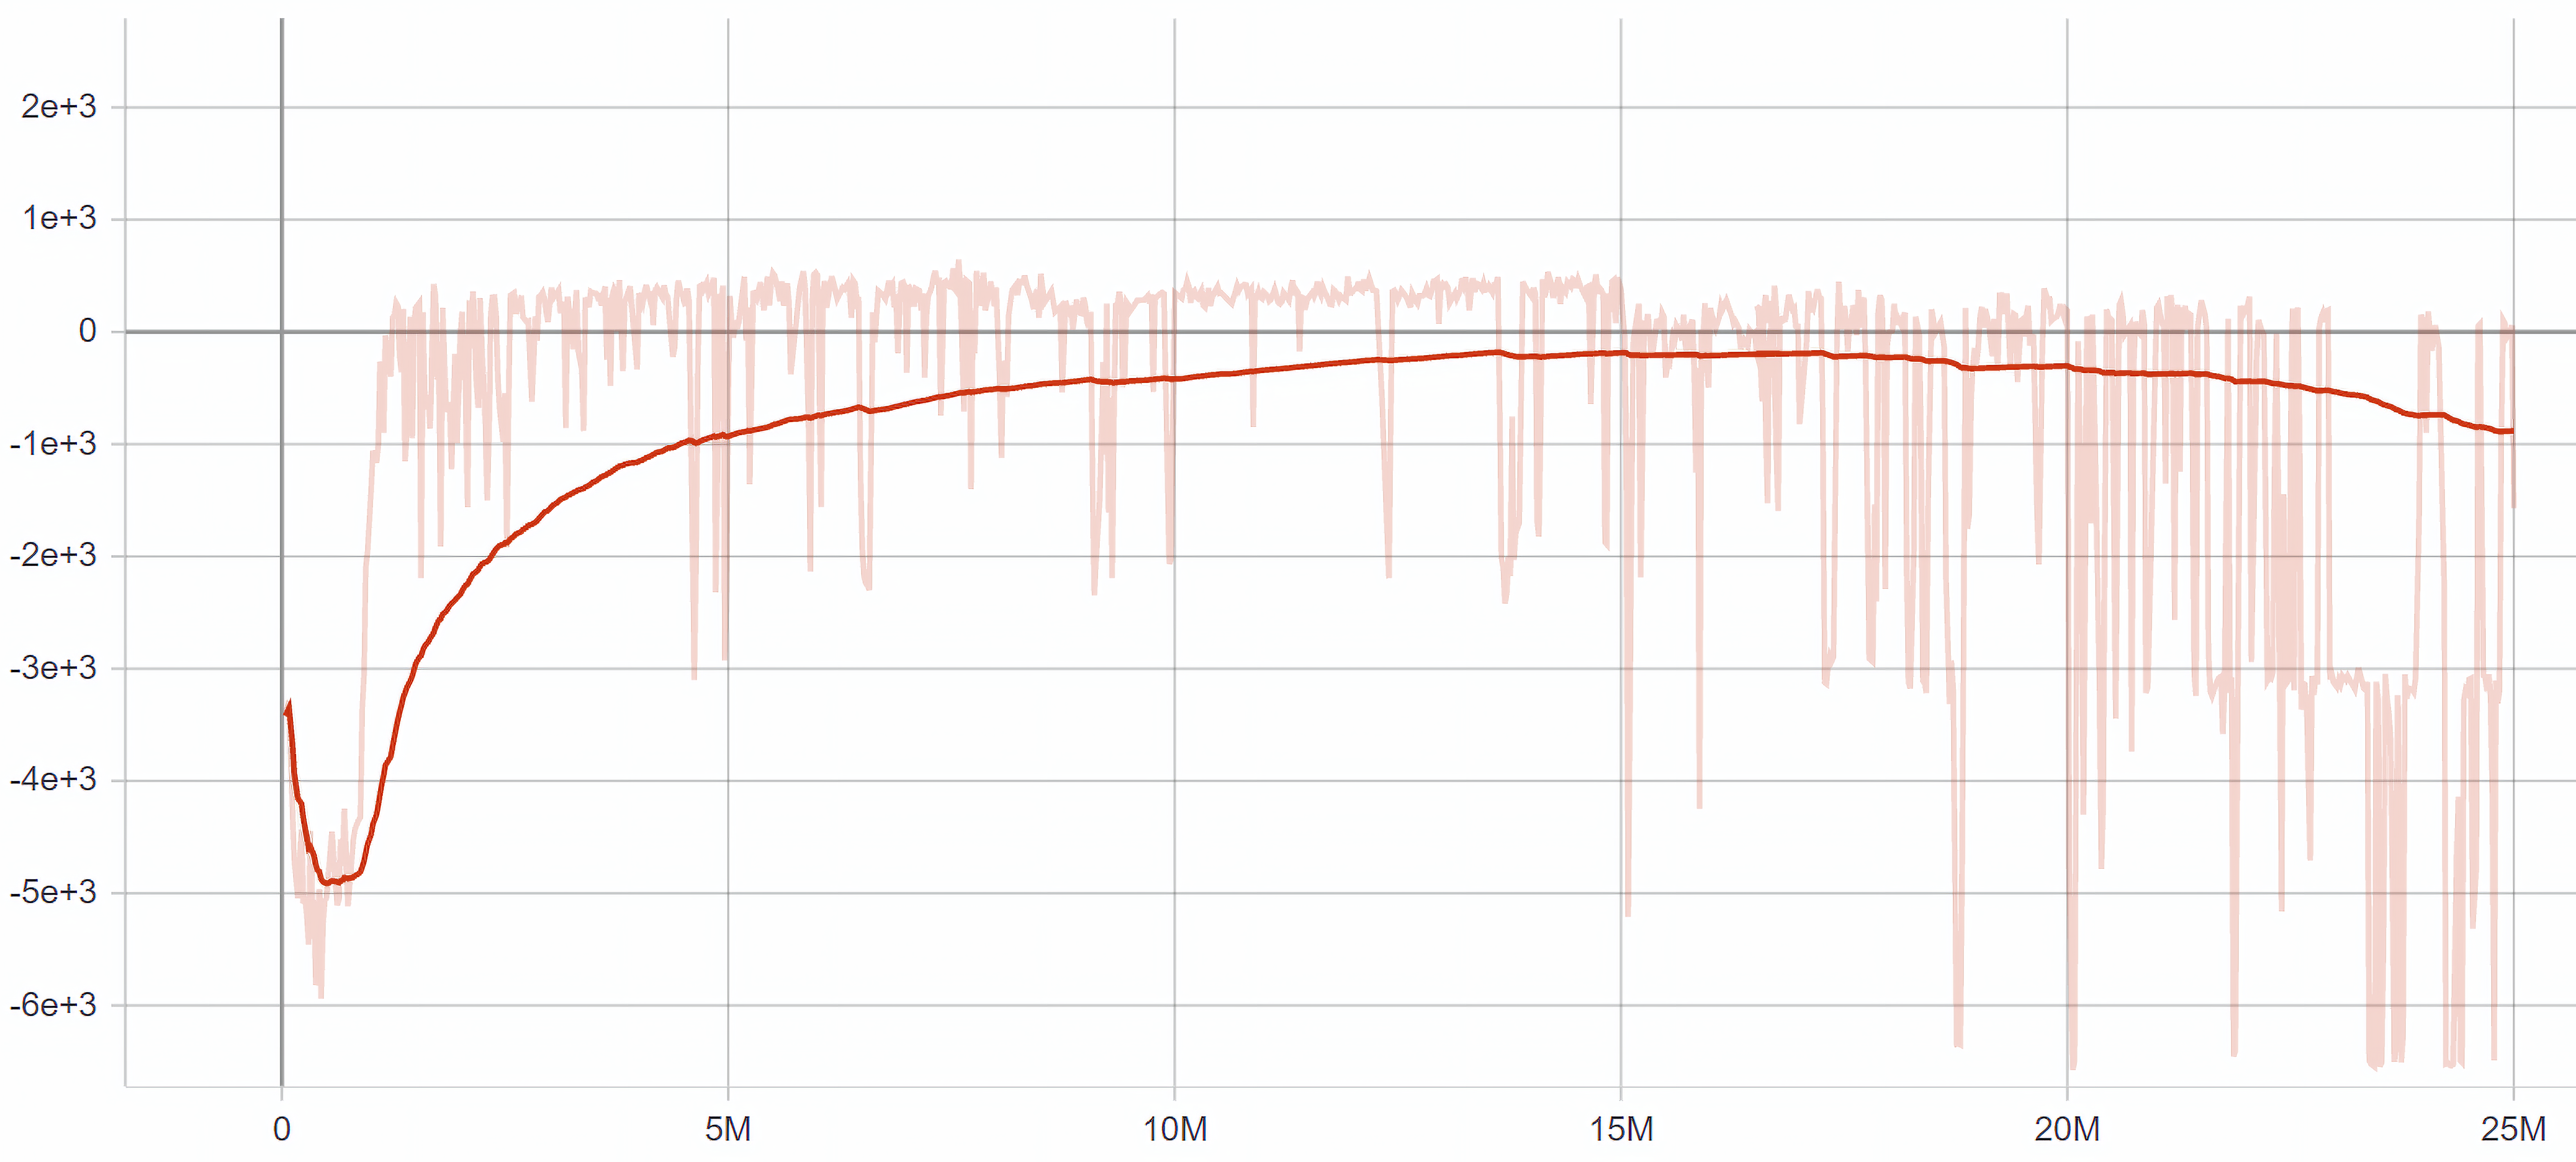
\includegraphics[scale=0.4]{Figures/Tensorboard4.PNG}
    \caption{Gap and Velocity Tracking of Test Case 3}
\end{figure}


\begin{comment}
\begin{figure}
\centering
\begin{subfigure}[b]{0.4\textwidth}
   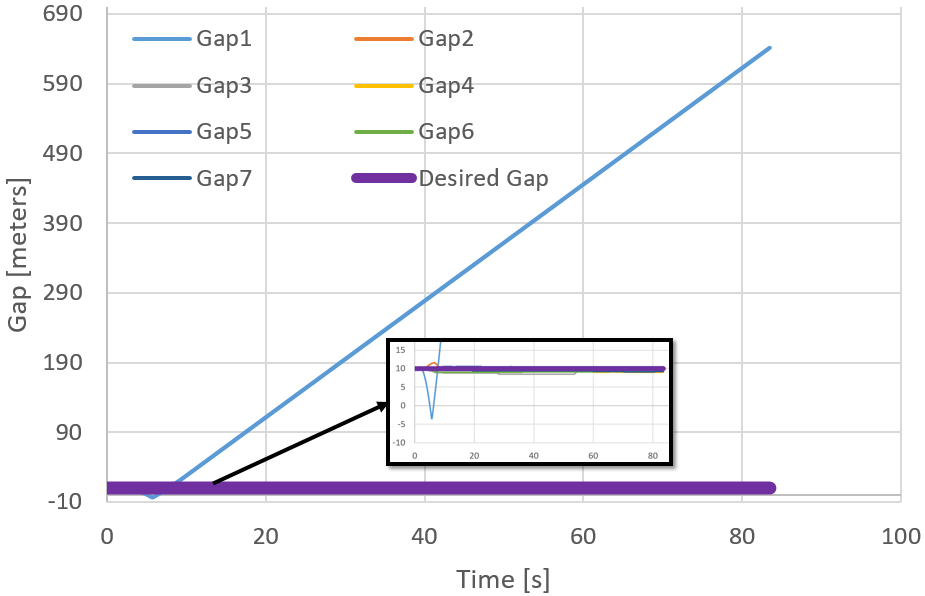
\includegraphics[width=1\linewidth]{Figures/EXP20_Gap3-u2.PNG}
   \label{fig:Ng1} 
\end{subfigure}

\begin{subfigure}[b]{0.4\textwidth}
   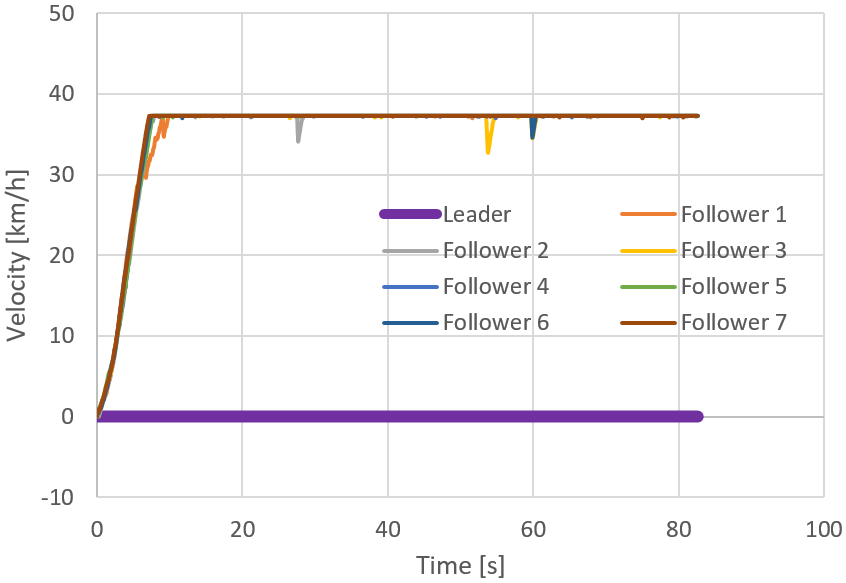
\includegraphics[width=1\linewidth]{Figures/EXP20_Vel-u2.PNG}
   \label{fig:Ng2}
\end{subfigure}

\caption[]{Gap and Velocity Tracking of Test Case 3}
\end{figure}
\end{comment}




%\subsection{SDCP Testing Experiments/ Test Track Results}
\subsection{Test Scenario 4 $|$ SDCP on the urban testing track}
Figure 16 shows the gaps and velocities of the platoon's vehicles driving on the test track and how followers try to maintain the desired gap with small margins, as shown in Table VIII, and the same velocity through all the taken maneuvers to drive safely through the consecutive tight turns, obstacles, and experience a new scenario of passing through a narrow way between two obstacles. In such a hard environment, vehicles give higher priority to ego performance of keeping driving safely through the whole track, collecting more positive rewards from reaching more checkpoints and reaching the finish line to gain the highest reward and avoid high negative rewards caused by crashing, than to focus only on maintaining the desired gap. Decentralized driving behavior and flexible spacing policy effects are observed in the performance of the vehicles as each vehicle has its own objectives and behavior that respect the platoon's regulations and formation while focusing on solo driving performance. Based on this acquired behavior and driving skills through training using deep RL, vehicles achieve both individual stability and string stability.


\begin{comment}
\begin{table}[H]
\centering
\caption{Performance metrics of the test scenario 4} 
\resizebox{8.75cm}{!}{
\begin{tabular} {|c||c|c|c|c|c|c|} 
 \hline
 \textbf{Evaluation metrics} & \textbf{$RMSE_{Gap1}$} & \textbf{$RMSE_{Gap2}$} & \textbf{$Std_{Gap1}$} & \textbf{$Std_{Gap2}$} & \textbf{$Stall_{Gap1}$} & \textbf{$Stall_{Gap2}$}\\
\hline
Value (meters) & 2.49 & 0.71 & 0.79 & 0.59 & 1.8 & 0.1\\ 
\hline
\textbf{Evaluation metrics} & \textbf{$RMSE_{Gap3}$} & \textbf{$RMSE_{Gap4}$} & \textbf{$Std_{Gap3}$} & \textbf{$Std_{Gap4}$} & \textbf{$Stall_{Gap3}$} & \textbf{$Stall_{Gap4}$}\\
\hline
Value (meters) & 1.94 & 2.34 & 1.25 & 1.41 & 1 & 3.8\\ 
\hline
\textbf{Evaluation metrics} & \textbf{$RMSE_{Gap5}$} & \textbf{$RMSE_{Gap6}$} & \textbf{$Std_{Gap5}$} & \textbf{$Std_{Gap6}$} & \textbf{$Stall_{Gap5}$} & \textbf{$Stall_{Gap6}$}\\
\hline
Value (meters) & 0.53 & 1.27 & 0.46 & 1.01 & -0.3 & -1.4\\ 
\hline
\textbf{Evaluation metrics} & \textbf{$RMSE_{Gap7}$} & \textbf{$Std_{Gap7}$} & \textbf{$Stall_{Gap7}$} & & &\\
\hline
Value (meters) & 2.03 & 1.53 & 1.6 & & &\\
\hline
\end{tabular} }
\end{table}
\end{comment}

\begin{table}
\centering
\caption{Performance metrics of the test scenario 4} 
\resizebox{8.55cm}{!}{
\renewcommand{\arraystretch}{2.25}
\Large
\begin{tabular} {|c||c|c|c|c|c|c|c|} 
 \hline
 \textbf{Evaluation metrics} & \textbf{$RMSE_{Gap1}$} & \textbf{$RMSE_{Gap2}$} & \textbf{$RMSE_{Gap3}$} & \textbf{$RMSE_{Gap4}$} & \textbf{$RMSE_{Gap5}$} & \textbf{$RMSE_{Gap6}$} & \textbf{$RMSE_{Gap7}$}\\
\hline
Value (meters) & 2.49 & 0.71 & 1.94 & 2.34 & 0.53 & 1.27 & 2.03\\ 
\hline
\textbf{Evaluation metrics} & \textbf{$Std_{Gap1}$} & \textbf{$Std_{Gap2}$} & \textbf{$Std_{Gap3}$} & \textbf{$Std_{Gap4}$} & \textbf{$Std_{Gap5}$} & \textbf{$Std_{Gap6}$} & \textbf{$Std_{Gap7}$}\\
\hline
Value (meters) & 0.79 & 0.59 & 1.25 & 1.41 & 0.46 & 1.01 & 1.53\\ 
\hline
\textbf{Evaluation metrics} & \textbf{$Max_{Gap5}$} & \textbf{$Max_{Gap6}$} & \textbf{$Max_{Gap5}$} & \textbf{$Max_{Gap6}$} & \textbf{$Max_{Gap5}$} & \textbf{$Max_{Gap6}$} & \textbf{$Max_{Gap7}$}\\
\hline
Value (meters) & 4.3 & -2.6 & 3.2 & 3.9 & -2.6 & -3.5 & -3.9\\ 
\hline
\textbf{Evaluation metrics} & \textbf{$Stall_{Gap1}$} & \textbf{$Stall_{Gap2}$} & \textbf{$Stall_{Gap3}$} & \textbf{$Stall_{Gap4}$} & \textbf{$Stall_{Gap5}$} & \textbf{$Stall_{Gap6}$} & \textbf{$Stall_{Gap7}$}\\
\hline
Value (meters) & 1.8 & 0.1 & 1 & 3.8 & -0.3 & -1.4 & 1.6\\
\hline
\end{tabular} }
\end{table}

\begin{comment}
talk about limitations here of decentralization that limits synchronization between vehicles
\end{comment}


\begin{figure}
    \centering
    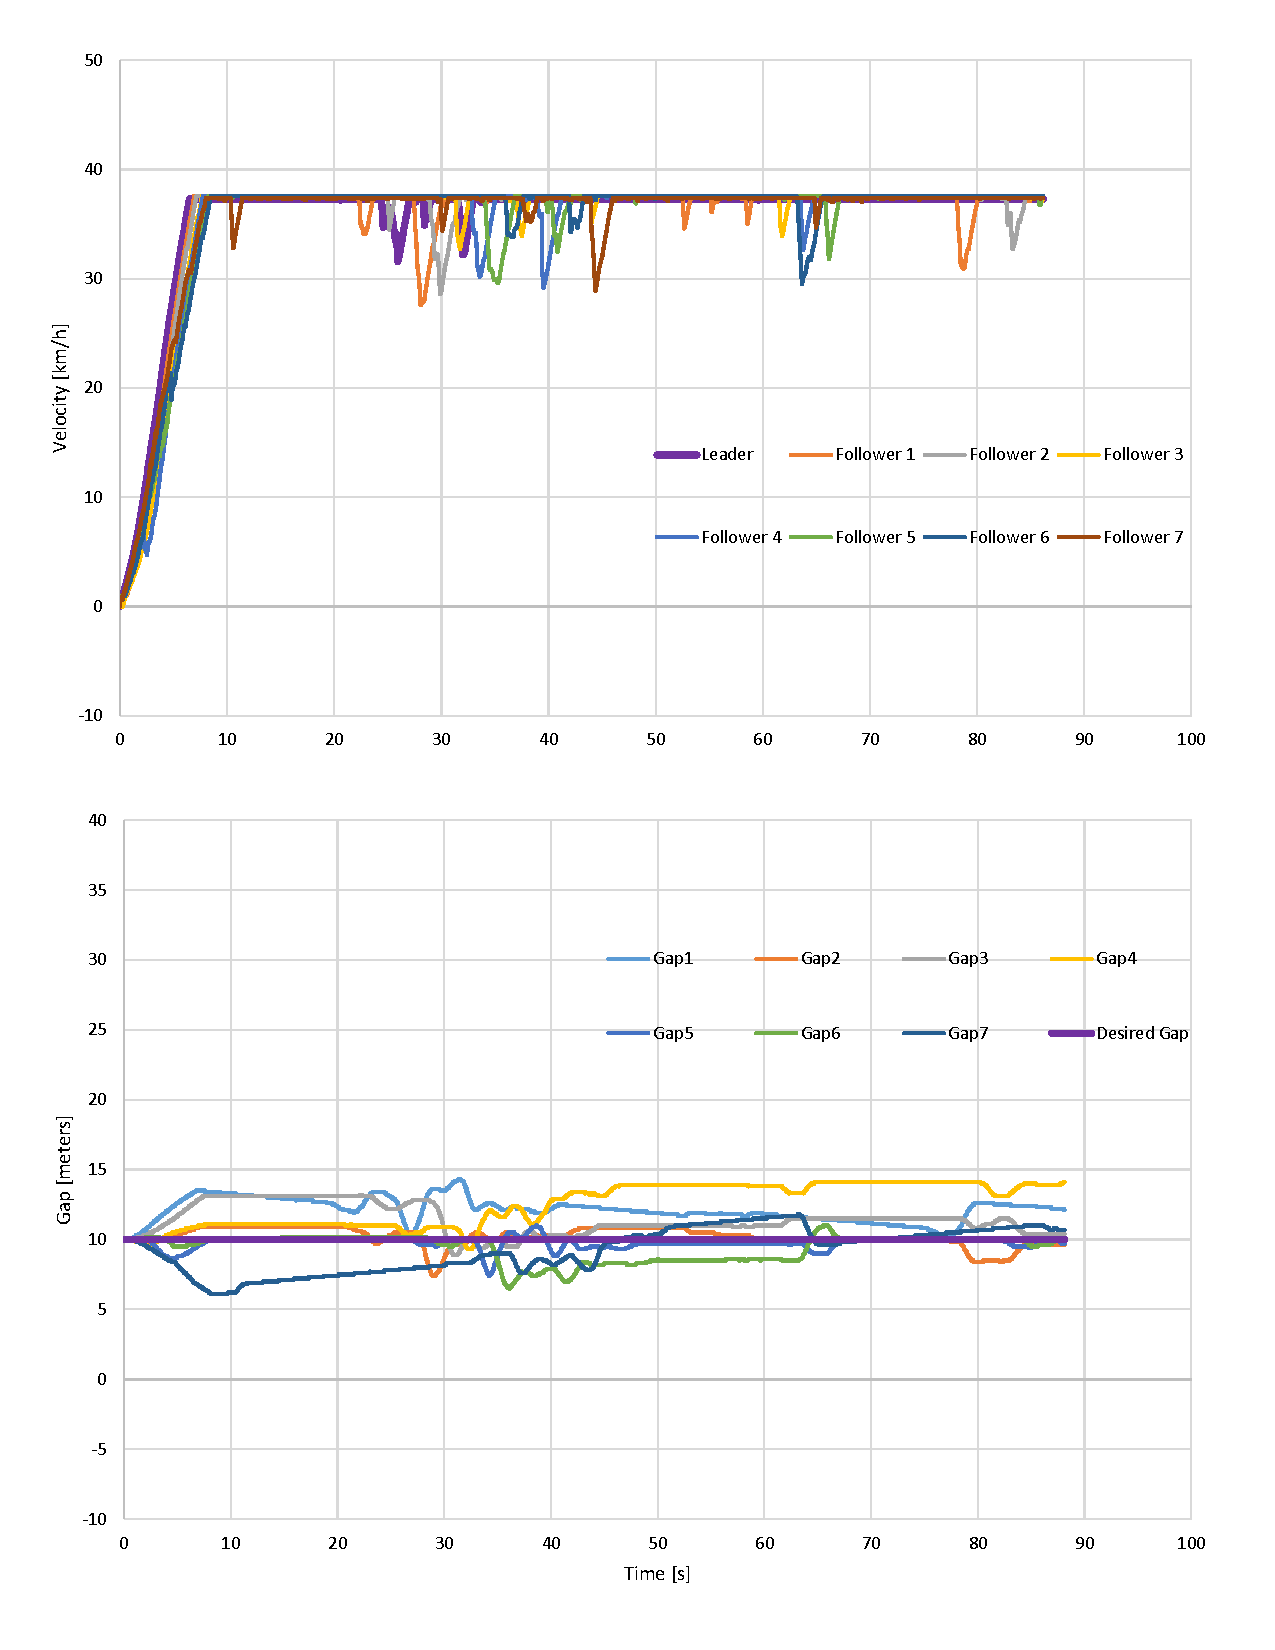
\includegraphics[width=1\linewidth]{Figures/Exp15Final_compressed.pdf}
    %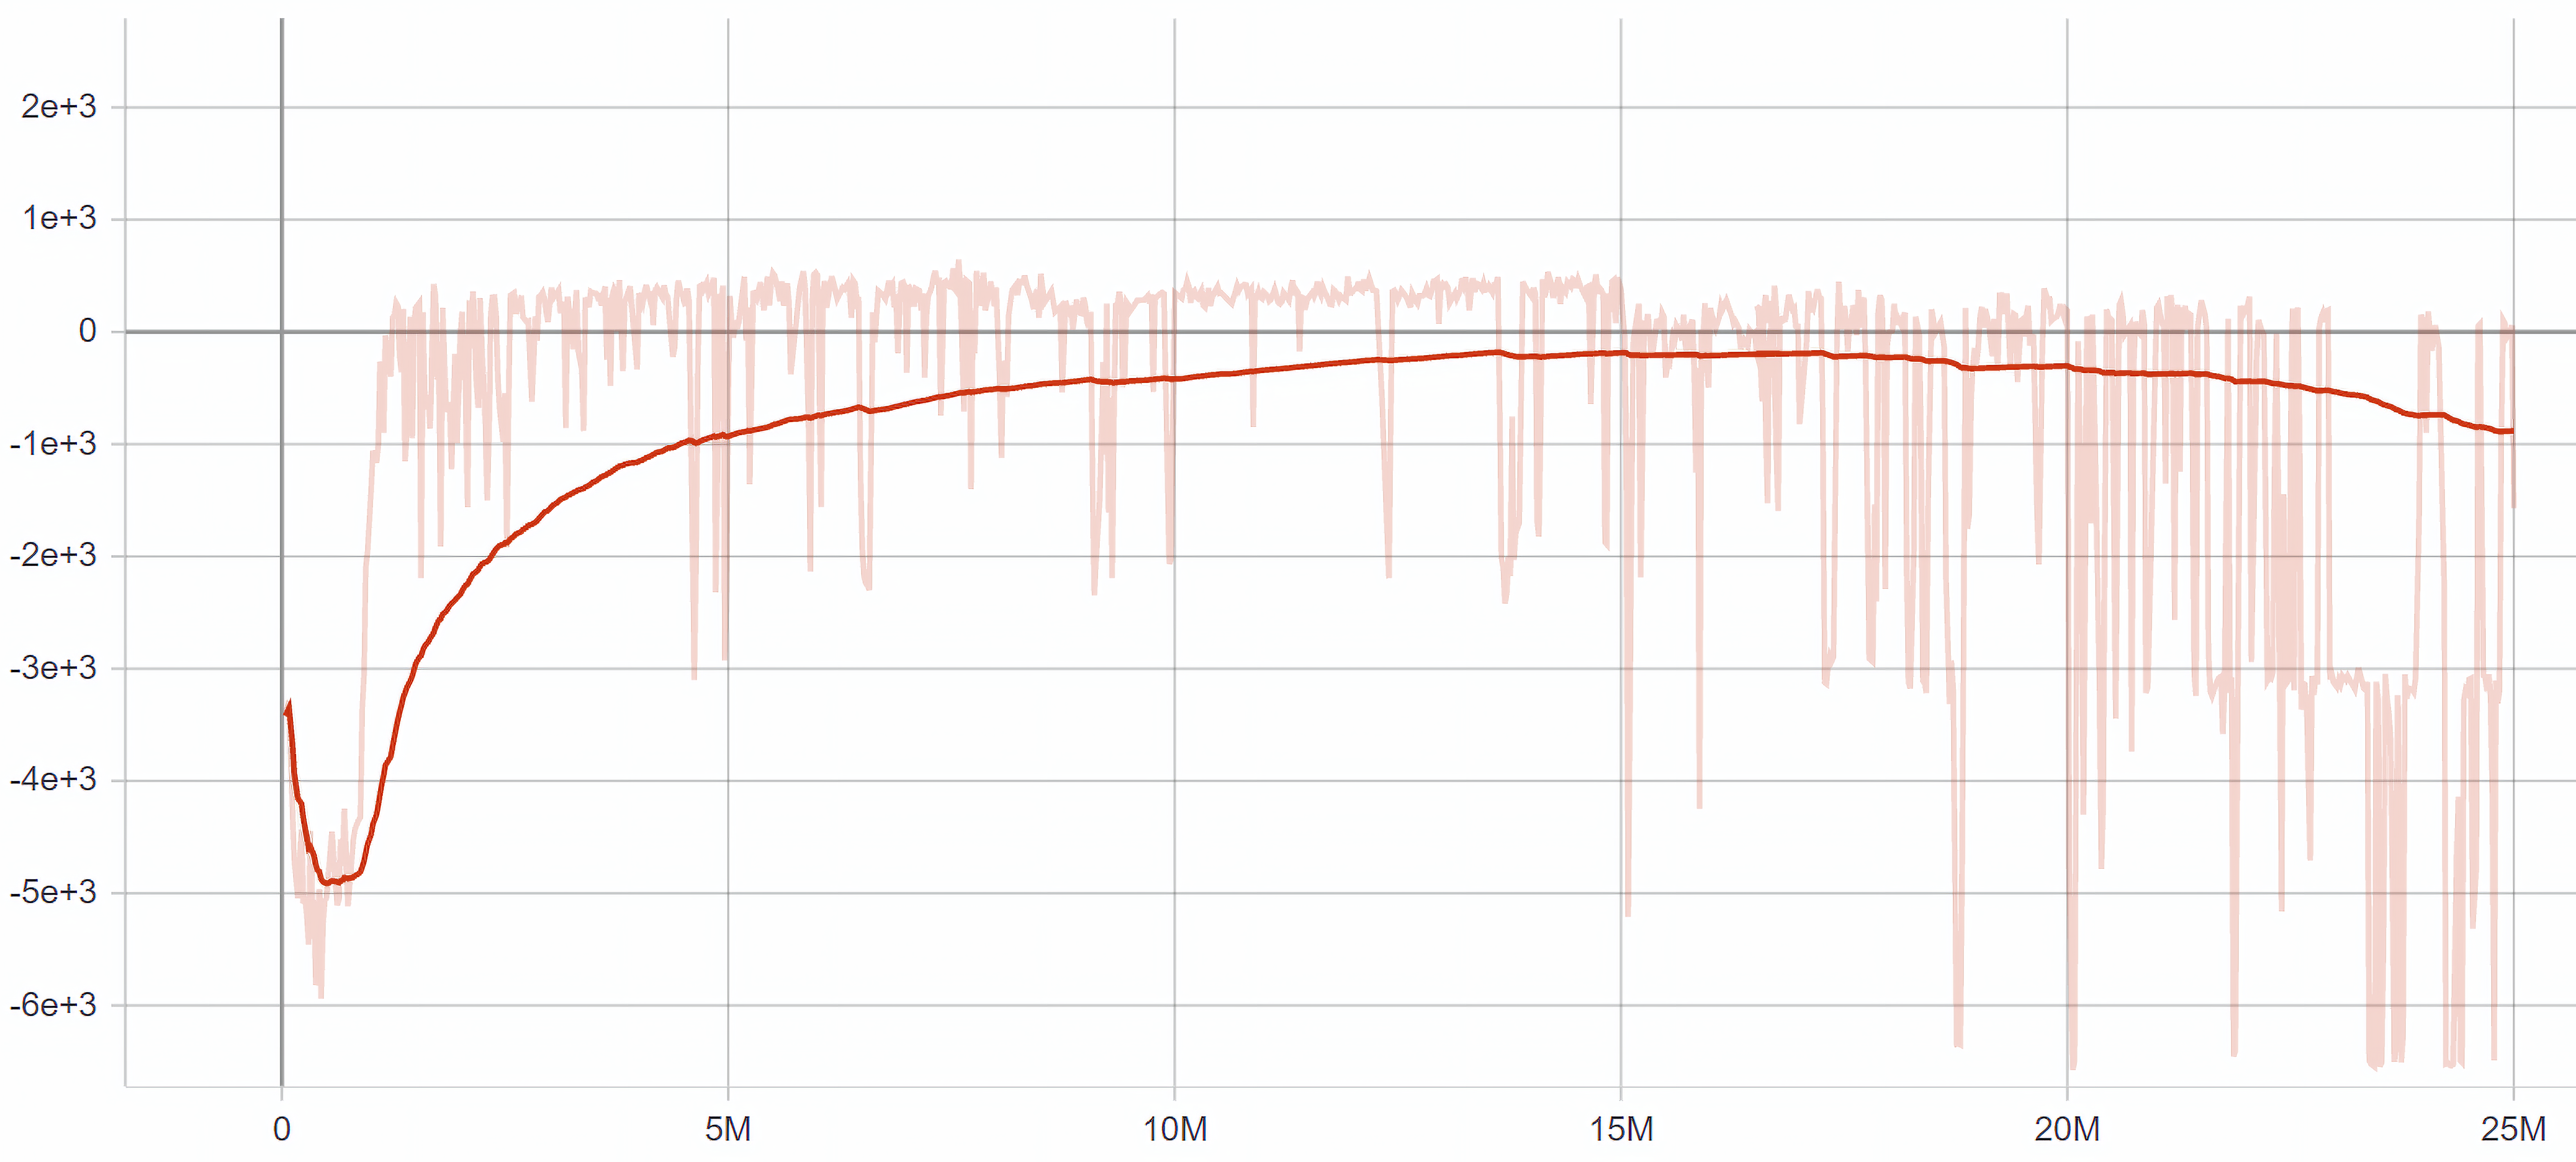
\includegraphics[scale=0.4]{Figures/Tensorboard4.PNG}
    \caption{Gap and Velocity Tracking of Test Case 4}
\end{figure}

\begin{comment}
\begin{figure}[H]
\centering
\begin{subfigure}[b]{0.45\textwidth}
   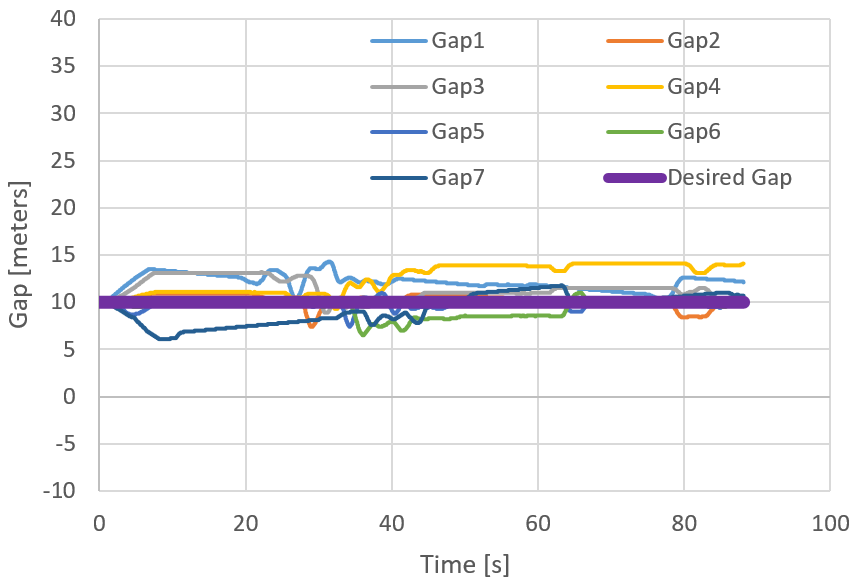
\includegraphics[width=1\linewidth]{Figures/GapFigure5.PNG}
   \label{fig:Ng1} 
\end{subfigure}

\begin{subfigure}[b]{0.45\textwidth}
   \includegraphics[width=1\linewidth]{VelocityFigure5.png}
   \label{fig:Ng2}
\end{subfigure}

\caption[]{Gap and Velocity Tracking of Test Case 4}
\end{figure}
\end{comment}


\subsection{Test Scenario 5 $|$ Traffic Congestion}
A platoon with eight vehicles was subjected to drive on the testing track, as shown in Figure 9 while being connected based on predecessor follower-based sharing and caring communication topology and without being connected to measure how the communication and cooperation between vehicles affect traffic congestion and safe driving. Results show that one accident occurred between the last two vehicles in the platoon when there was no communication applied between vehicles, and with communication, no accidents occurred and the throughput increased by 33\%.

\begin{table}[H]
\centering
\caption{Number of Accidents for each test case} 
\resizebox{8.55cm}{!}{
\renewcommand{\arraystretch}{2.25}
\Large
\begin{tabular} {|c||c|c|c|c|c|c|} 
 \hline
 \textbf{Test Case no.} & \textbf{Test Case 1} & \textbf{Test Case 2} & \textbf{Test Case 3} & \textbf{Test Case 4} & \textbf{Test Case 5 (V2V on)} & \textbf{Test Case 5 (V2V off)}\\
\hline
 Accidents & 0 & 0 & 0 & 0 & 0 & 1\\
\hline
\end{tabular} }
\end{table}

%Modify it
\subsection{Discussion}
Numerical results in the previous tables (III-IX) show the metrics of performance of all the gap errors, the velocities tracking of the vehicles in the platoon, and the number of crashes for each test case study through the whole driving distance.\\
SDCP completely succeeded in reaching zero crashes in all the case studies, and this boosts the gained behavior that gives high priority to safe driving through the applied sharing and caring communication topology and the reward signals that give high penalties on crashes. RMSE, standard deviation, and stalled gap errors for all gaps are relatively small compared to the total driving distances and based on the influence of the adopted flexible spacing policy which gives more driving flexibility for the vehicles within the platoon, as long as no accidents occur, except for the first follower in test scenario 3 which gets a very high penalty on the gap error between it and the leader, predecessor vehicle, but since follower's behavior is decentralized and has more courage to keep drive safely than to stop and wait for the leader to lead the platoon, the first follower continued driving as if it is the leader and followers cooperatively followed each other till reached the finish line and all gain the highest positive rewards in the environment.\\
Decentralization improves the vehicle's solo performance, but it affects the synchronization between vehicles and this is one of the limitations of decentralized systems. Vehicles' behavior in some situations, was greedy for their performance and cumulative reward, however, on the other hand, decentralization with the help of the novel predecessor follower-based sharing and caring communication topology made it applicable to have a robust scalable platoon, guaranteeing platoon stability, and safe driving by achieving zero accidents through the five conducted test case seniors (excluding when V2V is off in test case 5).



\subsection{Work Limitations}
There are some limitations in the conducted work listed as follows:
\begin{itemize}
    \item Roads in simulation work must have borders since only depth sensors are used.
    \item All simulation work is conducted on roads with only 2 lanes.
    \item Testing track created in Unity can only handle the presence of a platoon with a maximum of 8 vehicles and the track must get bigger to handle more vehicles for stable empirical experiments.
\end{itemize}



























\begin{comment}
\begin{table}[H]
\centering
\caption{Test Cases Evaluation based on RMSE and Number of Crashes} 
\resizebox{8.5cm}{!}{
\begin{tabular} {|c||c|c|c|c|} 
 \hline
 \textbf{Evaluation metrics} & \textbf{Test Scenario 1} & \textbf{Test Scenario 2} & \textbf{Test Scenario 3} & \textbf{Test Scenario 4}\\
\hline
Driving distance & 750m & 750m & 750m & 1000m\\ 
\hline
Crashes & 0 & 0 & 0 & 0\\
\hline
$RMSE_{Gap1}$ & 1.66 & 1.89 & 347.22 & 2.49\\
\hline
$RMSE_{Gap2}$ & 1.07 & 2.27 & 0.32 & 0.71\\
\hline
$RMSE_{Gap3}$ & 0.37 & 2.16 & 1.11 & 1.94\\
\hline
$RMSE_{Gap4}$ & 0.65 & 1.73 & 0.55 & 2.34\\
\hline
$RMSE_{Gap5}$ & 0.45 & 0.91 & 0.49 & 0.53\\
\hline
$RMSE_{Gap6}$ & 0.38 & 0.49 & 0.84 & 1.27\\
\hline
$RMSE_{Gap7}$ & 0.34 & 0.13 & 0.64 & 2.03\\
\hline
\end{tabular} }
\end{table}
\end{comment}



%Add MAE, Std, ....








































\begin{comment}
First test case is to show SDCP performance on the test track shown in Figure ? which is full of hard maneuvers for the platoon to handle while keeping the desired gap and same velocities as possible and the other three cases are tested on a track of a straight forward road with no obstacles and turns to be able to focus more on the core principles of SDCP which are scalable platoon length, decentralization and cooperation through proposed sharing and caring communication topology.

\subsection{Test Scenario 1 (scalable platoon length)}

SDCP is firstly tested on a track of a straight forward road with no obstacles and turns as a simple case study to evaluate their performance on keeping the desired gap and same velocity for all vehicles in the platoon.



%\subsection{Test Scenario 1 (scalable length of platoon)}
In training process, platoon's length is of three vehicles, one leader and 2 followers. In this first test scenario for SDCP performance evaluation the length of the platoon is increased to eight vehicles, one leader and seven followers.
\end{comment}





\begin{comment}
training time 40476.215 s = 11h 14m 36s

The training for the ego vehicle controller took 2163 episodes with a total number of steps of 973,186
for approximately 9.5 hours. The final average reward based on Equation 4 was 326.8 as seen in
Figure 2. The initial conditions of the velocities and positions of the vehicles are randomly changed
before the beginning of each episode to ensure the reliability of the agent for any given realistic
scenario and prevent over-fitting of the model to certain scenarios. Thus, each episode has a different
initial gap error and different initial speed error.

\begin{figure}[H]
    \centering
    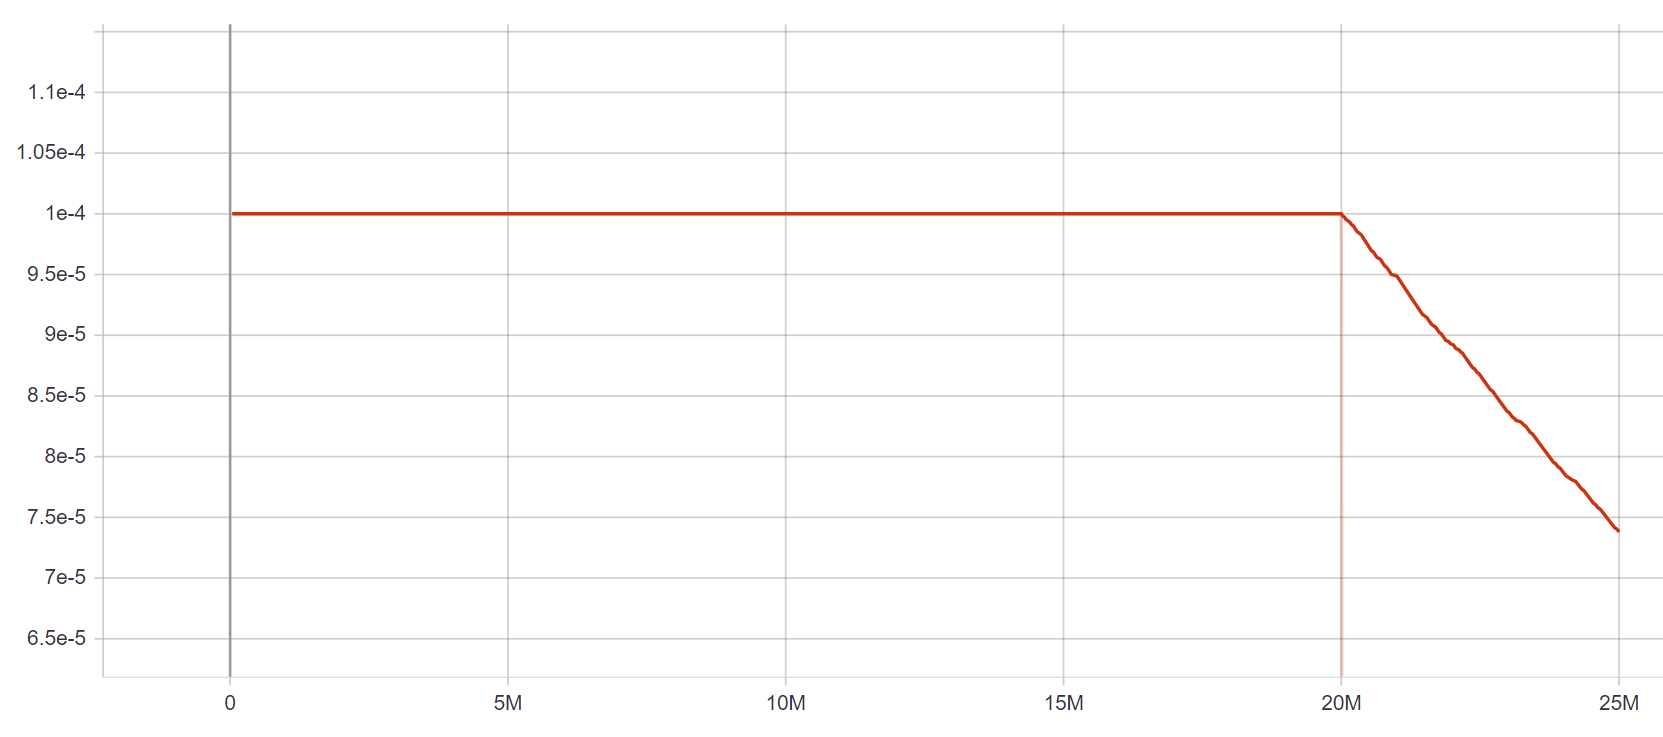
\includegraphics[width=8cm,height=5cm,keepaspectratio]{Figures/LR.PNG}
    %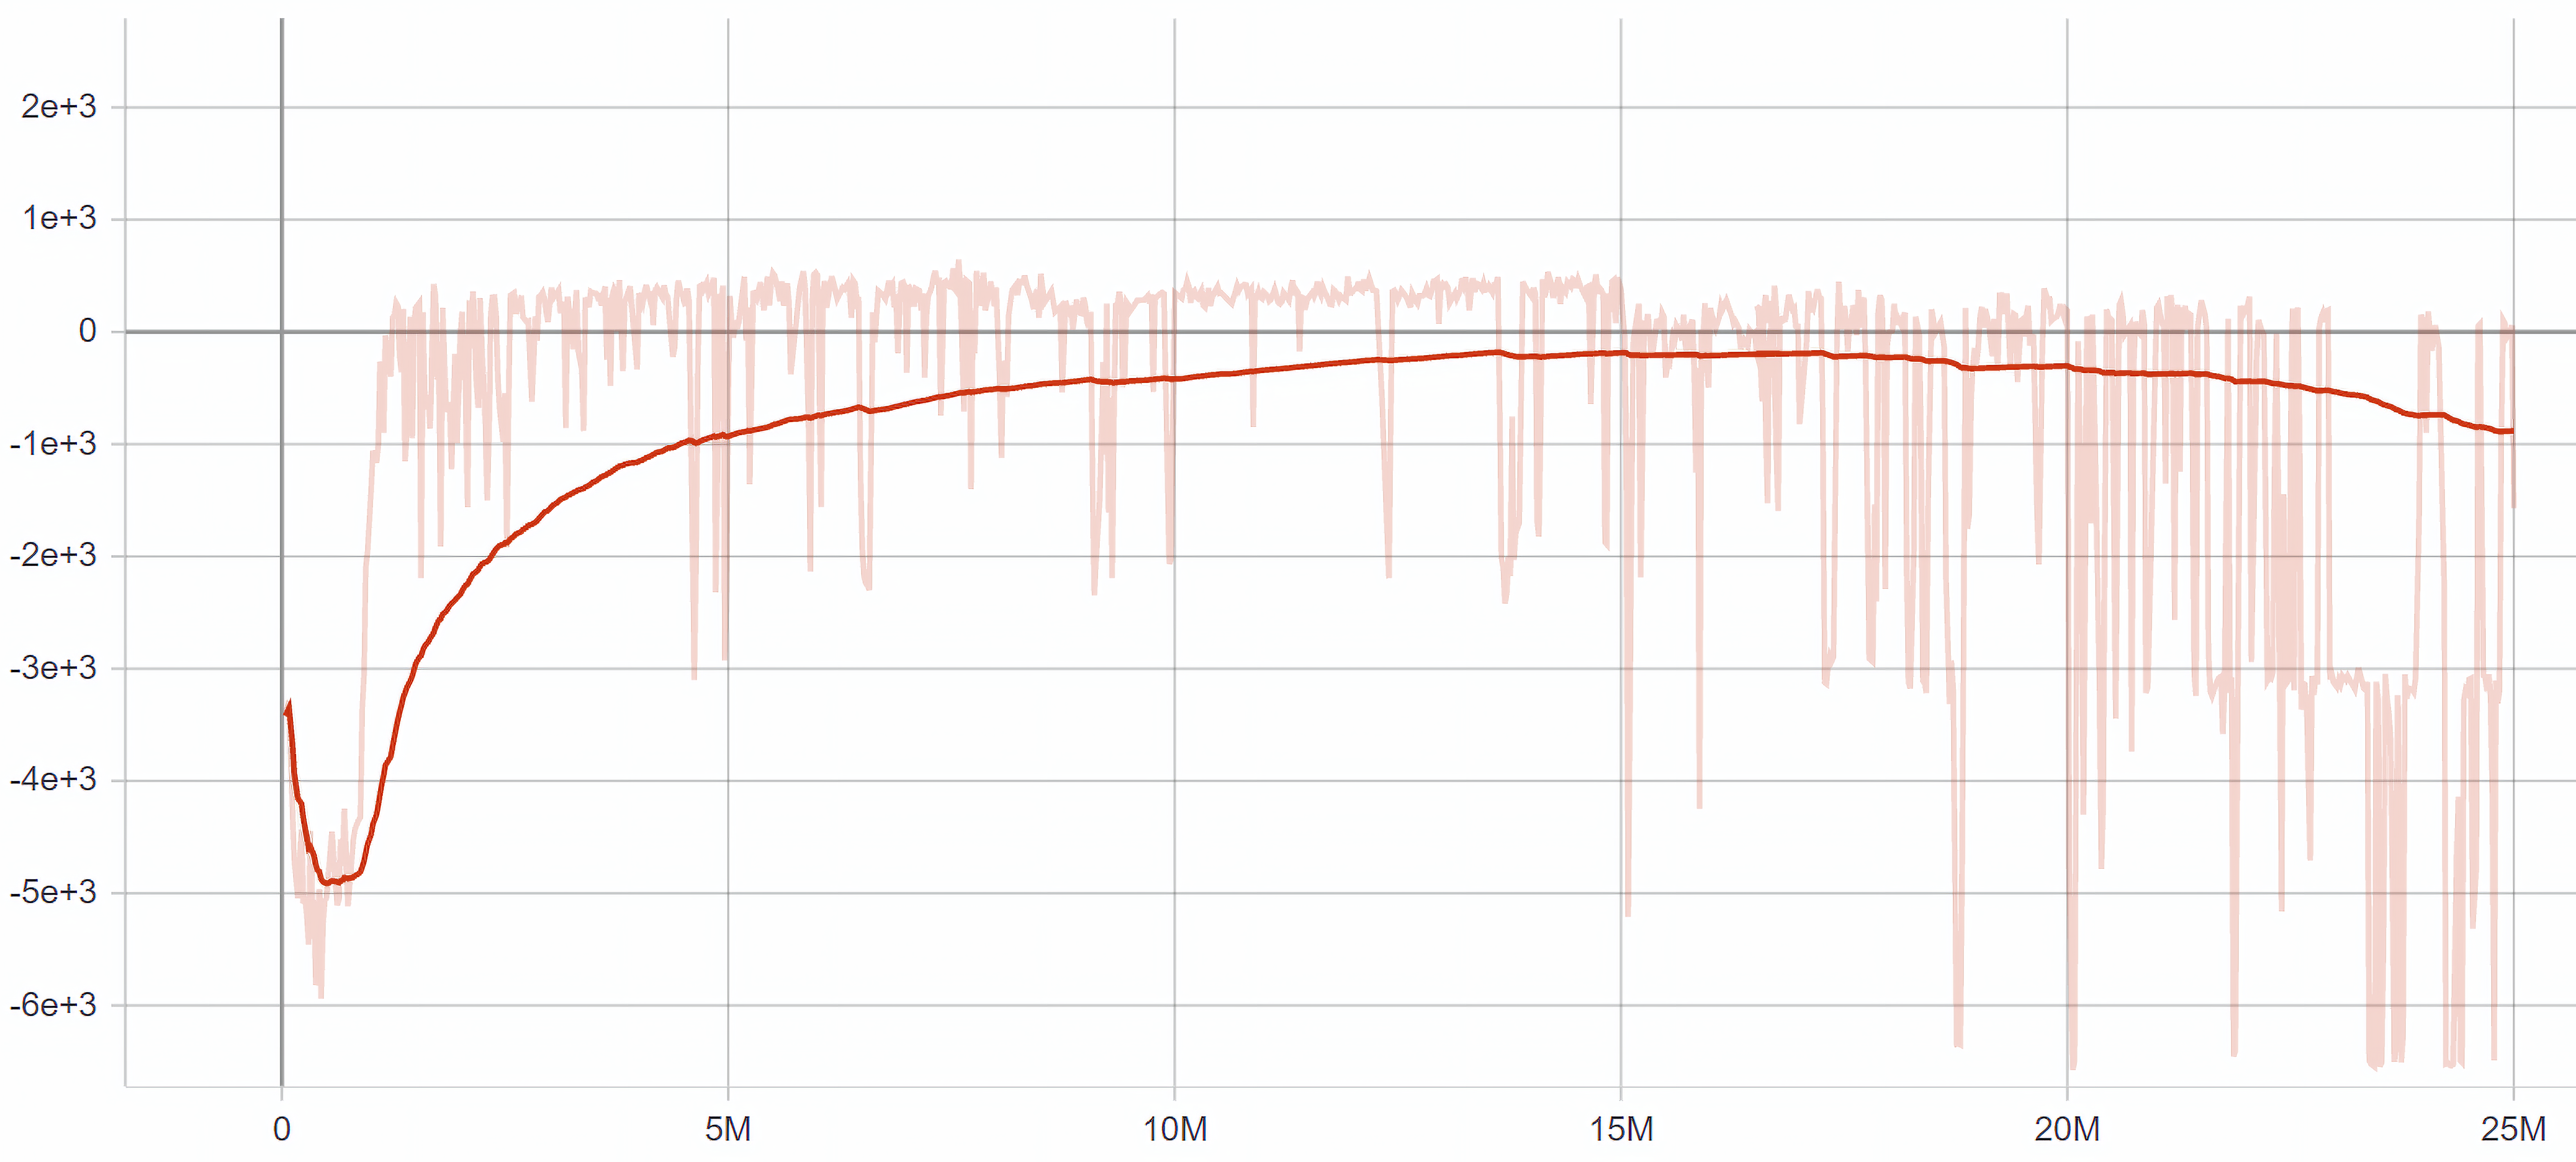
\includegraphics[scale=0.4]{Figures/Tensorboard4.PNG}
    \caption{Test Track}
    \label{fig:my_label}
\end{figure}


\begin{figure}[H]
    \centering
    %\includegraphics[width=8cm,height=5cm,keepaspectratio]{Figures/GapFigure(S)5.PNG}
    \includegraphics[scale=0.4]{Figures/GapFigure(S)5.PNG}
    \caption{Gaps of Platoon Vehicles}
    \label{fig:my_label}
\end{figure}

\begin{figure}[H]
    \centering
    %\includegraphics[width=8cm,height=5cm,keepaspectratio]{Figures/VelocityFigure(S)5.png}
    \includegraphics[scale=0.43]{Figures/VelocityFigure(S)5.png}
    \caption{Velocities of Platoon Vehicles}
    \label{fig:my_label}
\end{figure}



\begin{figure}[H]
    \centering
    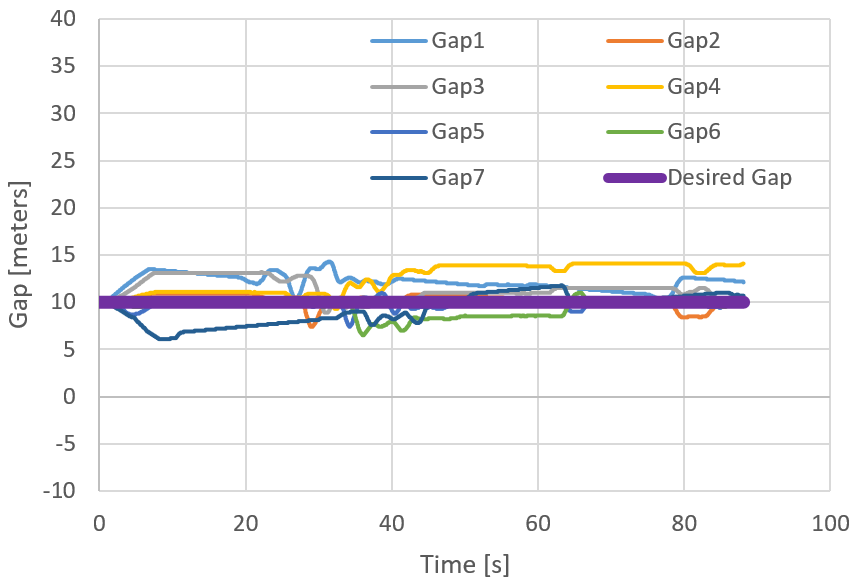
\includegraphics[scale=0.4]{Figures/GapFigure5.PNG}
    \caption{Test}
    \label{fig:my_label}
\end{figure}

\begin{figure}[H]
    \centering
    \includegraphics[scale=0.422]{Figures/VelocityFigure5.PNG}
    \caption{Test}
    \label{fig:my_label}
\end{figure}


\begin{table}[H]
\centering
\caption{Reward signals} 
\resizebox{8.5cm}{!}{
\begin{tabular} {|c|c|c|c|c|c|c|c|} 
 \hline
 Crashes & $RMSE_{Gap1}$ &$RMSE_{Gap2}$&$RMSE_{Gap3}$&$RMSE_{Gap4}$&$RMSE_{Gap5}$&$RMSE_{Gap6}$&$RMSE_{Gap7}$\\
\hline
0 & 0 & 0 & 0 & 0 & 0 & 0 & 0\\
\hline
\end{tabular} }
\end{table}


\end{comment}





\begin{comment}
To validate scalability, cooperation, and decentralization some cases studies is tested. Platoon length is increased to eight vehicles. Platoon formation and safe driving 

Also there are two more test case studies to be held to validate scalable length of the platoon, cooperation, and decentralization of the agents. First case study is to increase the length of the platoon to 8 vehicles and visualize gap and velocity error between them. Second case study is to test if the followers can drive without the leader.
\end{comment}


\begin{comment}
Evaluating performance of SDCP is measured by number of crashes which represents, speed error, gap error, robustness(change max velocity or starting positions, track structure, ....) (want to add more? ask others or review some papers). Add it to Results and Experiments? i think so to talk more about experiments


\textbf{validate your 3 concepts(scalability, decentralization, and sharing and caring effect on platoon performance. sharing and caring may be can not be validated except by remove caring and test, check if this is possible!!) on different scenarios, like video you sent to dr omar that validate decentralization and safety with respecting platoon formation and also this may validate Cooperative Adaptive Cruise Control (CACC)}

Mention that the pursuit of decentralization makes followers do not follow their predecessors aggressively. 
\end{comment}



























\begin{comment}
You need to proof that your results are good.
Either mention that it performs like humans and collect results from people.
Or compare your results to other papers work.
Or compare the difference between with out sharing and caring and with.
Mention that both are in a race, because behavior here may change like happened may decide to let other vehicle crash to win.
Your work contribute in Safe Driving point of view.

Compare results while you drive and check how many accidents happened compared with two Autonomous connected Vehicles.

Focus your work on influence of sharing and caring concept on multi-agent connected vehicles.

Create a video with all test cases and behaviors aroused of your experiments on unity.\\
e.g. part 1: when vehicles crash\\
part 2: afraid of crashing\\
part 3: cooperate while sharing and caring.\\
Apply these trained models on different roads and you can mention u used parallel environments to collect more data in shorter time.
\end{comment}
